\documentclass[]{book}
\usepackage{lmodern}
\usepackage{amssymb,amsmath}
\usepackage{ifxetex,ifluatex}
\usepackage{fixltx2e} % provides \textsubscript
\ifnum 0\ifxetex 1\fi\ifluatex 1\fi=0 % if pdftex
  \usepackage[T1]{fontenc}
  \usepackage[utf8]{inputenc}
\else % if luatex or xelatex
  \ifxetex
    \usepackage{mathspec}
  \else
    \usepackage{fontspec}
  \fi
  \defaultfontfeatures{Ligatures=TeX,Scale=MatchLowercase}
\fi
% use upquote if available, for straight quotes in verbatim environments
\IfFileExists{upquote.sty}{\usepackage{upquote}}{}
% use microtype if available
\IfFileExists{microtype.sty}{%
\usepackage{microtype}
\UseMicrotypeSet[protrusion]{basicmath} % disable protrusion for tt fonts
}{}
\usepackage[margin=1in]{geometry}
\usepackage{hyperref}
\hypersetup{unicode=true,
            pdftitle={Data Driven KPI (Key Performance Indicators) Insight \& Prediction},
            pdfauthor={Cevi Herdian, B. Sc, SFC (Scrum Fundamental Certified)},
            pdfborder={0 0 0},
            breaklinks=true}
\urlstyle{same}  % don't use monospace font for urls
\usepackage{natbib}
\bibliographystyle{apalike}
\usepackage{longtable,booktabs}
\usepackage{graphicx,grffile}
\makeatletter
\def\maxwidth{\ifdim\Gin@nat@width>\linewidth\linewidth\else\Gin@nat@width\fi}
\def\maxheight{\ifdim\Gin@nat@height>\textheight\textheight\else\Gin@nat@height\fi}
\makeatother
% Scale images if necessary, so that they will not overflow the page
% margins by default, and it is still possible to overwrite the defaults
% using explicit options in \includegraphics[width, height, ...]{}
\setkeys{Gin}{width=\maxwidth,height=\maxheight,keepaspectratio}
\IfFileExists{parskip.sty}{%
\usepackage{parskip}
}{% else
\setlength{\parindent}{0pt}
\setlength{\parskip}{6pt plus 2pt minus 1pt}
}
\setlength{\emergencystretch}{3em}  % prevent overfull lines
\providecommand{\tightlist}{%
  \setlength{\itemsep}{0pt}\setlength{\parskip}{0pt}}
\setcounter{secnumdepth}{5}
% Redefines (sub)paragraphs to behave more like sections
\ifx\paragraph\undefined\else
\let\oldparagraph\paragraph
\renewcommand{\paragraph}[1]{\oldparagraph{#1}\mbox{}}
\fi
\ifx\subparagraph\undefined\else
\let\oldsubparagraph\subparagraph
\renewcommand{\subparagraph}[1]{\oldsubparagraph{#1}\mbox{}}
\fi

%%% Use protect on footnotes to avoid problems with footnotes in titles
\let\rmarkdownfootnote\footnote%
\def\footnote{\protect\rmarkdownfootnote}

%%% Change title format to be more compact
\usepackage{titling}

% Create subtitle command for use in maketitle
\newcommand{\subtitle}[1]{
  \posttitle{
    \begin{center}\large#1\end{center}
    }
}

\setlength{\droptitle}{-2em}

  \title{Data Driven KPI (Key Performance Indicators) Insight \& Prediction}
    \pretitle{\vspace{\droptitle}\centering\huge}
  \posttitle{\par}
  \subtitle{Case Studies: Deutsche Bahn AG}
  \author{Cevi Herdian, B. Sc, SFC (Scrum Fundamental Certified)}
    \preauthor{\centering\large\emph}
  \postauthor{\par}
      \predate{\centering\large\emph}
  \postdate{\par}
    \date{2019-03-02}

\usepackage{booktabs}
\usepackage{amsthm}
\makeatletter
\def\thm@space@setup{%
  \thm@preskip=8pt plus 2pt minus 4pt
  \thm@postskip=\thm@preskip
}
\makeatother

\begin{document}
\maketitle

{
\setcounter{tocdepth}{1}
\tableofcontents
}
\chapter{Introduction}\label{introduction}

\section{Master's thesis statement of
originality}\label{masters-thesis-statement-of-originality}

I hereby confirm that I have written the accompanying thesis by myself,
without contributions from any sources other than those cited and
acknowledgements. This applies also to all graphics, drawings, maps and
images included in this thesis.

Berlin, 18. March 2019

Cevi Herdian, B. Sc, SFC (Scrum Fundamental Certified)

\section{Acknowledgments}\label{acknowledgments}

After fast 8 years of hard work with the study at Berlin University of
applied Sciences (HTW Berlin). From Studientkolleg till this Master, I
am now ready to face new challenges in the real world in my country
Indonesia. Writing this thesis has been interesting experience an also
my las work in university life. I have faced some difficulties but none
that have stopped me to complete this work. This thesis would not be
possible without help from the amazing people at that i meet in
University and at works.

This thesis based on my experience as internship and working student in
different company from 2015 till February 2019. And I took the use case
for this thesis in my last works in Deutsche Bahn from September 2019
till February 2019.

I would like to announce special thanks to Fathimah Dzakiyyah, my
beloved wife. And all of my family. I would also like to thank
Prof.~Dr.~Christians and Prof.~Dr.~Beate Bergter who has been inspring
me.

Last but not least I would like to thank my friends, Christ, Mathel,
Jabr, Ouafaa, and Hourya. They has been a continuous source of
inspiration and always been very helpful.

\section{Abstract}\label{abstract}

\textbf{Background: }Big Data can be defined as high Volume and Variety
of data that can be brought together and analyzed at high Velocity to
discover patterns and make better decisions. Deutsche Bahn as a
multinational company have also data growth from the company activities.
The KPI (Key Performances Indicator) helps a big data to more
understable in easily visualization. A right KPI should act as a gage,
helping company understand whether the company is taking the right path
toward the strategic goals. I have decided to investigate further of how
Deutsche Bahn operates with KPIs from they Big Data.

\textbf{Purpose: } The purpose of this thesis is to examine the
reception of Big Data Key Performance Indicators used at Deutsche Bahn
Headquarters. Investigate how Big Data KPIs evaluate their way of daily
monitoring. See if there is room for further improvements and also if
the findings are applicable in other company (another Deutsche Bahn
company).

\textbf{Method: } I decided to do only quantitative-approach when
collecting data. The quantitative data were retrieved from SAP Business
Object Web Intelligence Database. Because of data privacy at Deutsche
Bahn, the data that I used in this thesis isn't data from Deutsche Bahn,
but I tried to get similar manner data from another sources. In Use Case
part I created the analysis for problem solving from scratch (from the
very beginning, especially without making use of or relying on any
previous work for assistance).

\textbf{Conclusions: }

Deutsche Bahn uses KPIs in order to Increase sales, profit and to get
useful information from their big data that can be analyzed. It is up to
each and every sub departments to decide if and how they want to work
with the KPIs. Deutsche Bahn Headquarters is successful when operating
with big data KPIs. The teams get motivated by working with big data KPI
and feel that they can affect the outcome to at least a sufficient
extent. There are not many negative things to say about how Deutsche
Bahn Headquarters operates with KPIs but there is room for improvements.
We believe that other departments might be inspired of how Deutsche Bahn
Headquarters operates with KPIs.

\chapter{Data is everywhere}\label{data-is-everywhere}

Do you have smartphone? Off course, this kind of Ask is not relevant in
this era. From our Laptop, Tablet, PC or Handphone. This devices creates
more data nowadays. Data is more bigger and bigger. The world contains
an astronomical amount of data, an amount that grows larger and larger
each day. This Big Data has changed the way the world interacts,
uncovered breakthroughs in fast all of our life, from ecommerce,
medicine, genetic, financial etc.

The principle of Big Data works that the more you have data about
anything or any situation, the more accurately you get new
\textbf{insights} and make \textbf{predictions} about what will happen
in the future. Also revealed new ways to understand trends in business
and in our daily lives. By comparing more and more data and creating
relationships that were previously hidden enable us to learn and make
more smarter decisions on targeting business values such as sales,
production, or financial situations.

\begin{quote}
Based on forbes.com only \textbf{53\%} have big data strategies around
the world. The top use case are retail, social analysis, and predictive
maintenance.
\end{quote}

Key points include the following:

\begin{itemize}
\tightlist
\item
  \textbf{Reporting, dashboards, advanced visualization end-user
  ``self-service'' and data warehousing are the top five technologies
  and initiatives strategic to business intelligence (Figure 1.1).}
\end{itemize}

\begin{figure}
\centering
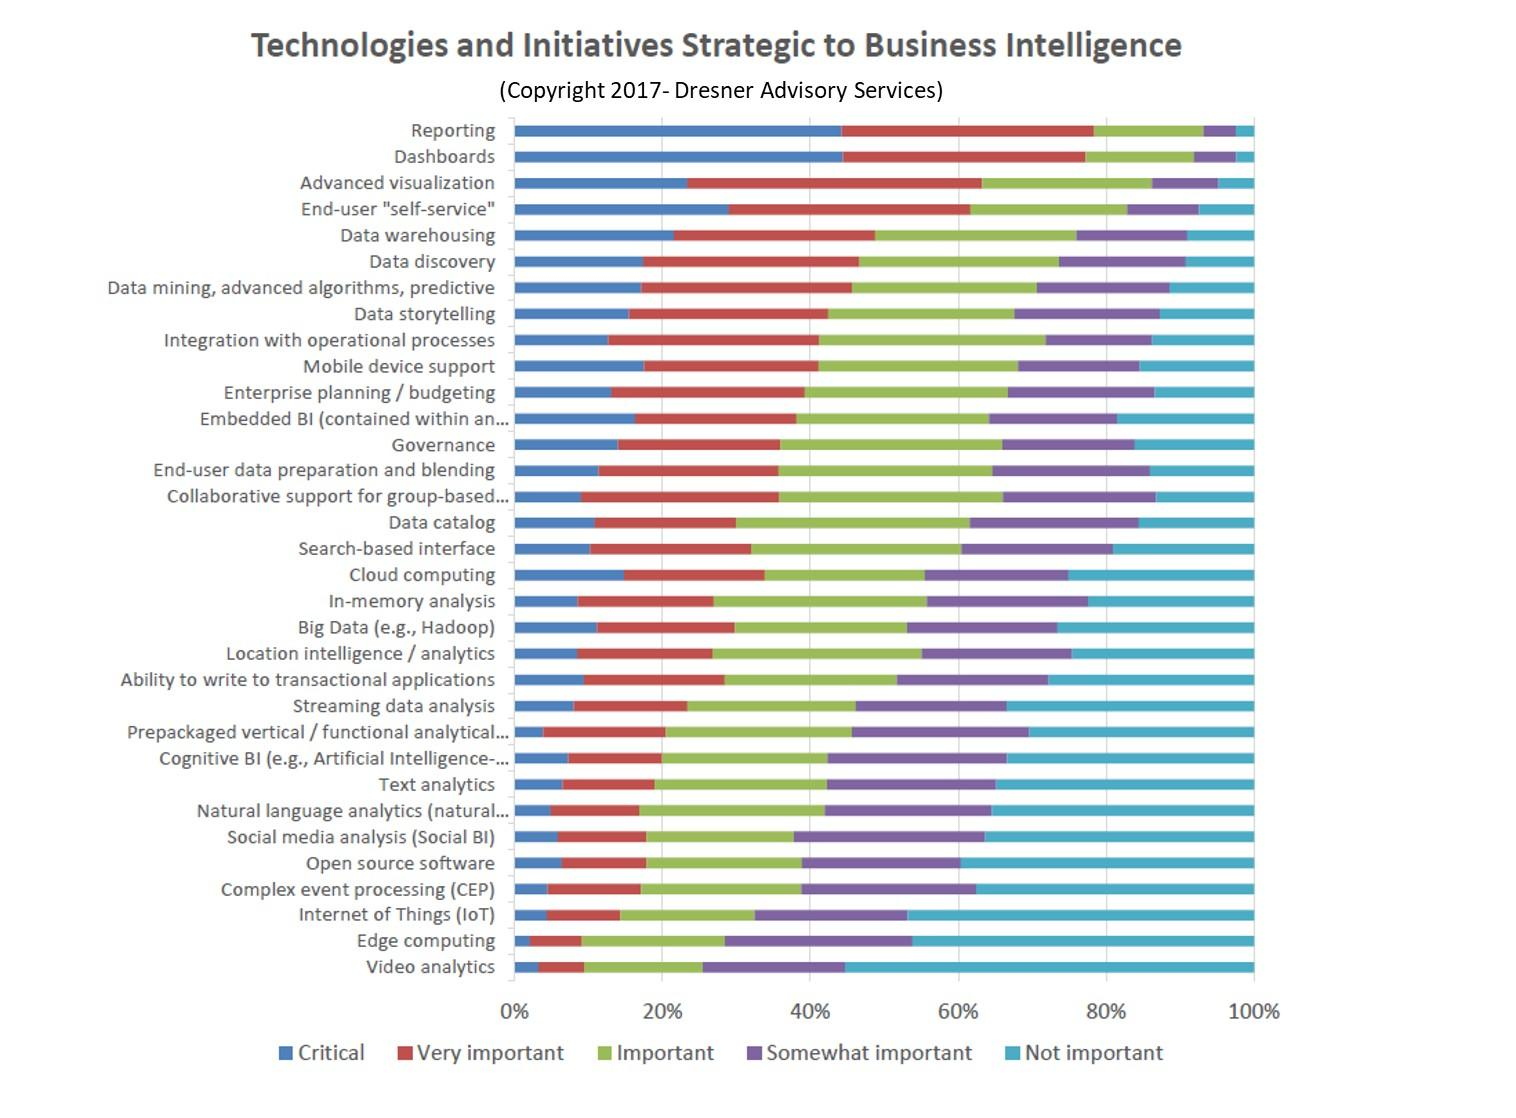
\includegraphics{1.jpg}
\caption{}
\end{figure}

\begin{itemize}
\tightlist
\item
  \textbf{53\% of companies are using big data analytics today, up from
  17\% in 2015 with Telecom and Financial Services industries fueling
  the fastest adoption (Figure 1.2).}
\end{itemize}

\begin{figure}
\centering
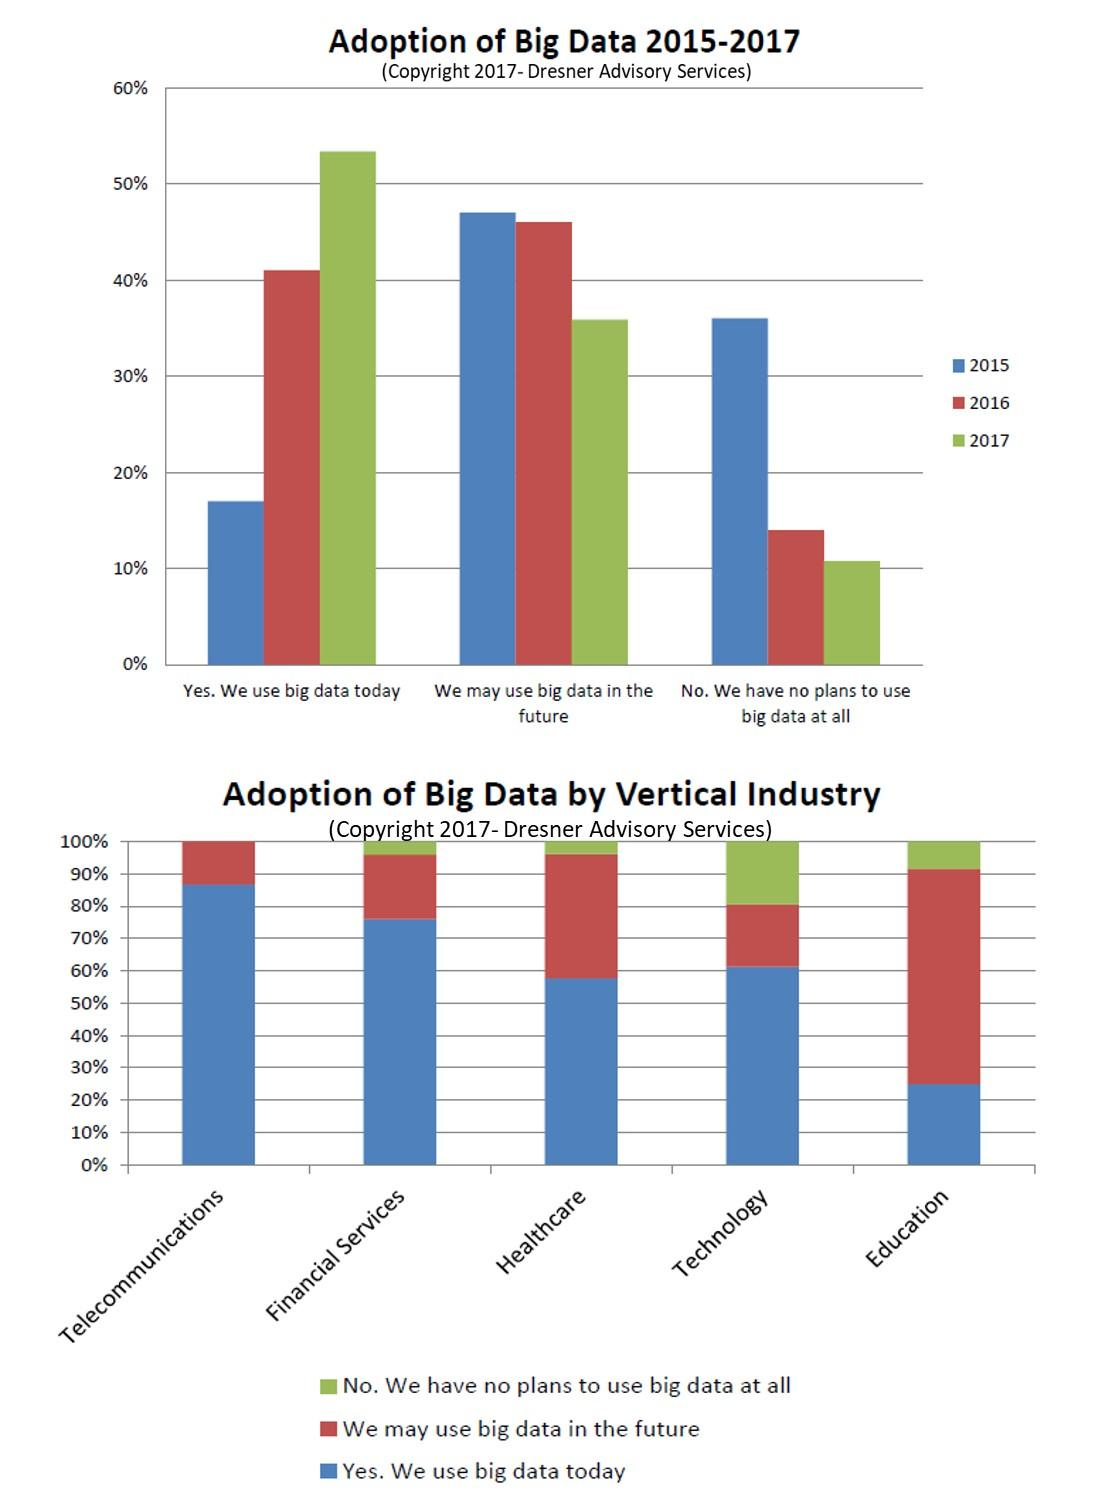
\includegraphics{2.jpg}
\caption{}
\end{figure}

\begin{itemize}
\tightlist
\item
  \textbf{Data warehouse optimization is considered the most important
  big data analytics use case in 2017, followed by customer/social
  analysis and predictive maintenance (Figure 1.3).}
\end{itemize}

\begin{figure}
\centering
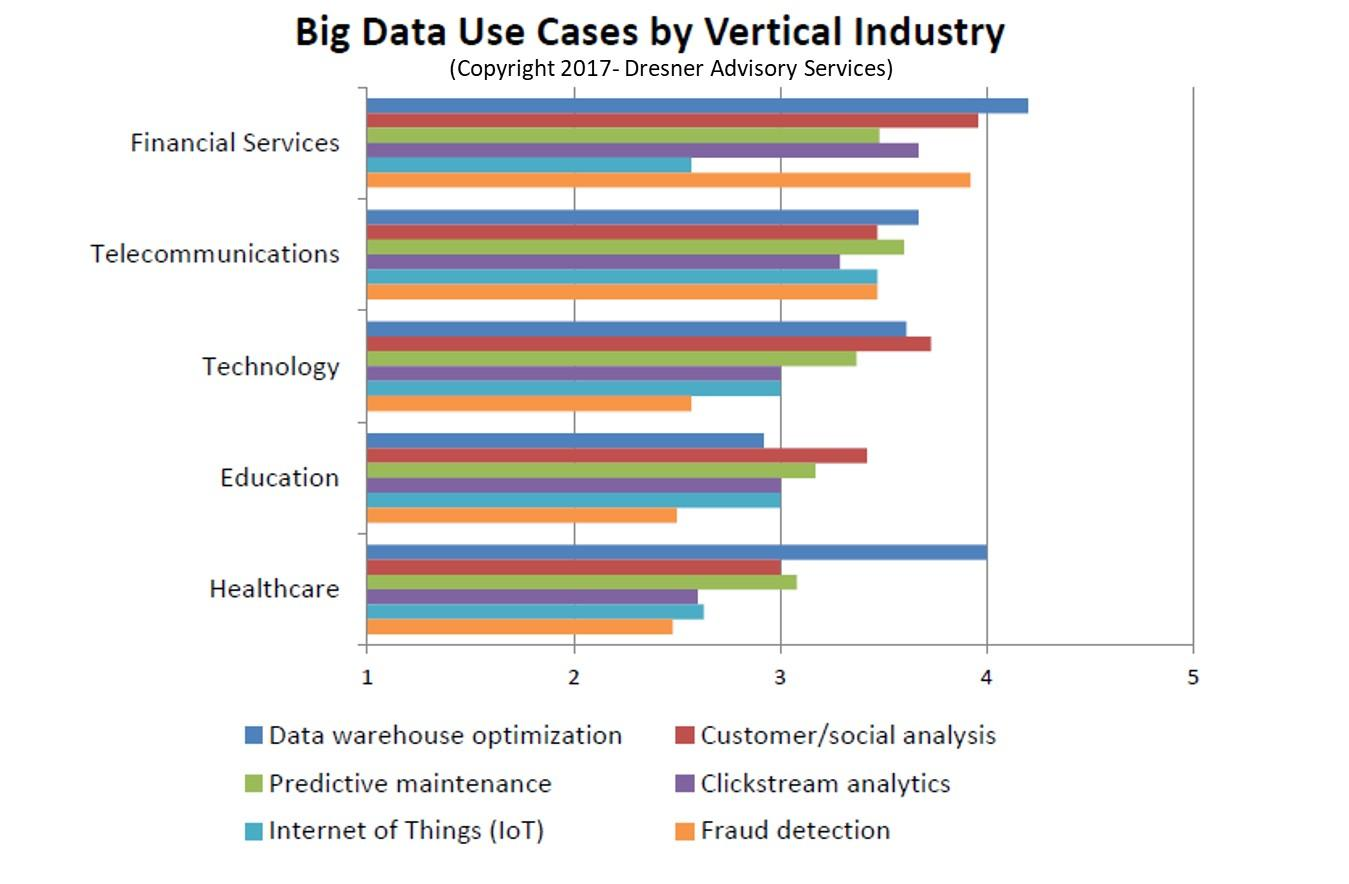
\includegraphics{3.jpg}
\caption{}
\end{figure}

\begin{itemize}
\tightlist
\item
  \textbf{Big data analytics use cases vary significantly by industry
  with data warehouse optimization dominating Financial Services,
  Healthcare, and Customer/social analysis is the leading use case in
  Technology-based companies (Figure 1.4).}
\end{itemize}

\begin{figure}
\centering
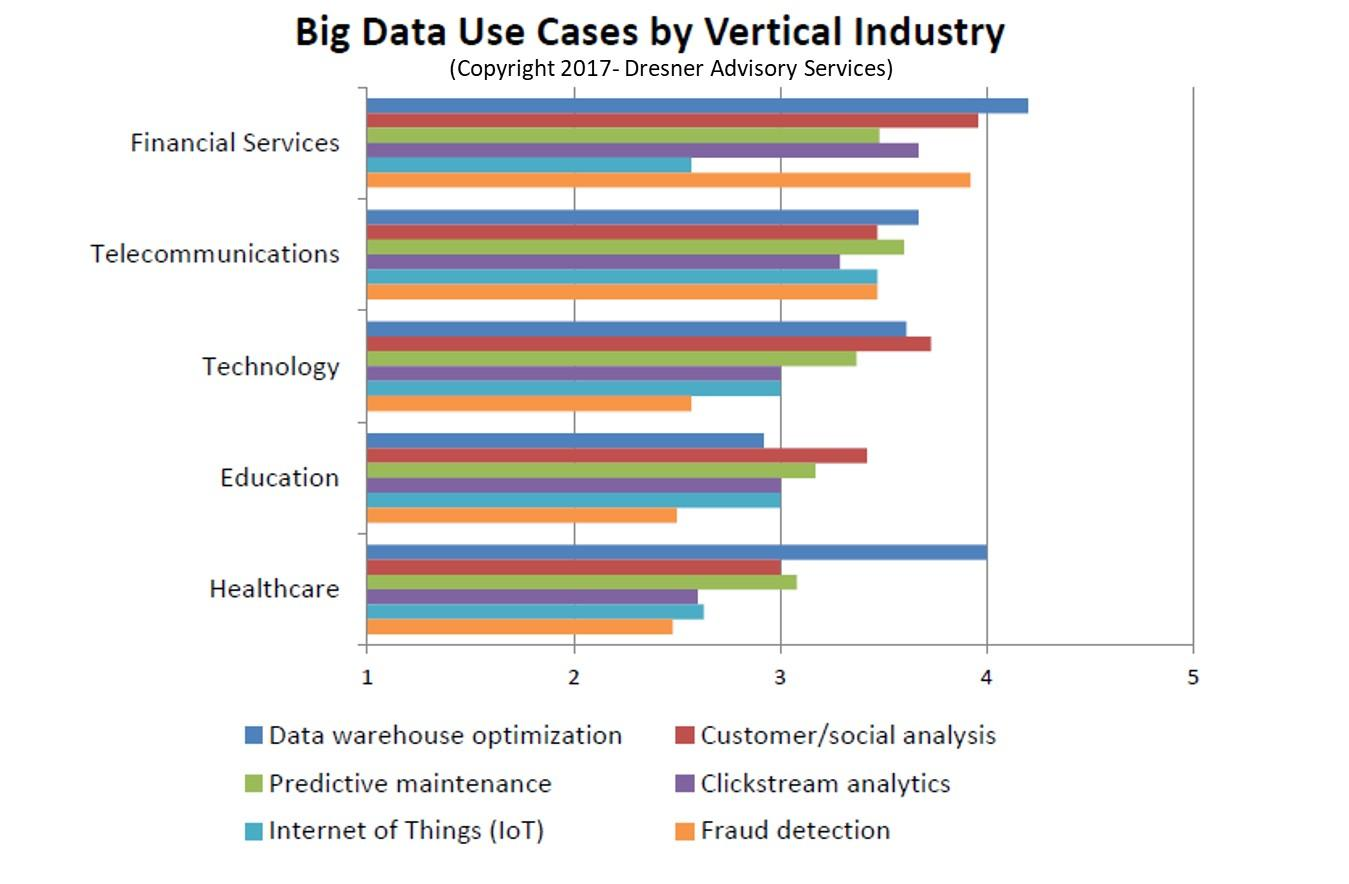
\includegraphics{4.jpg}
\caption{}
\end{figure}

\begin{itemize}
\tightlist
\item
  \textbf{Spark, MapReduce, and Yarn are the three most popular software
  frameworks today (Figure 1.5).}
\end{itemize}

\begin{figure}
\centering
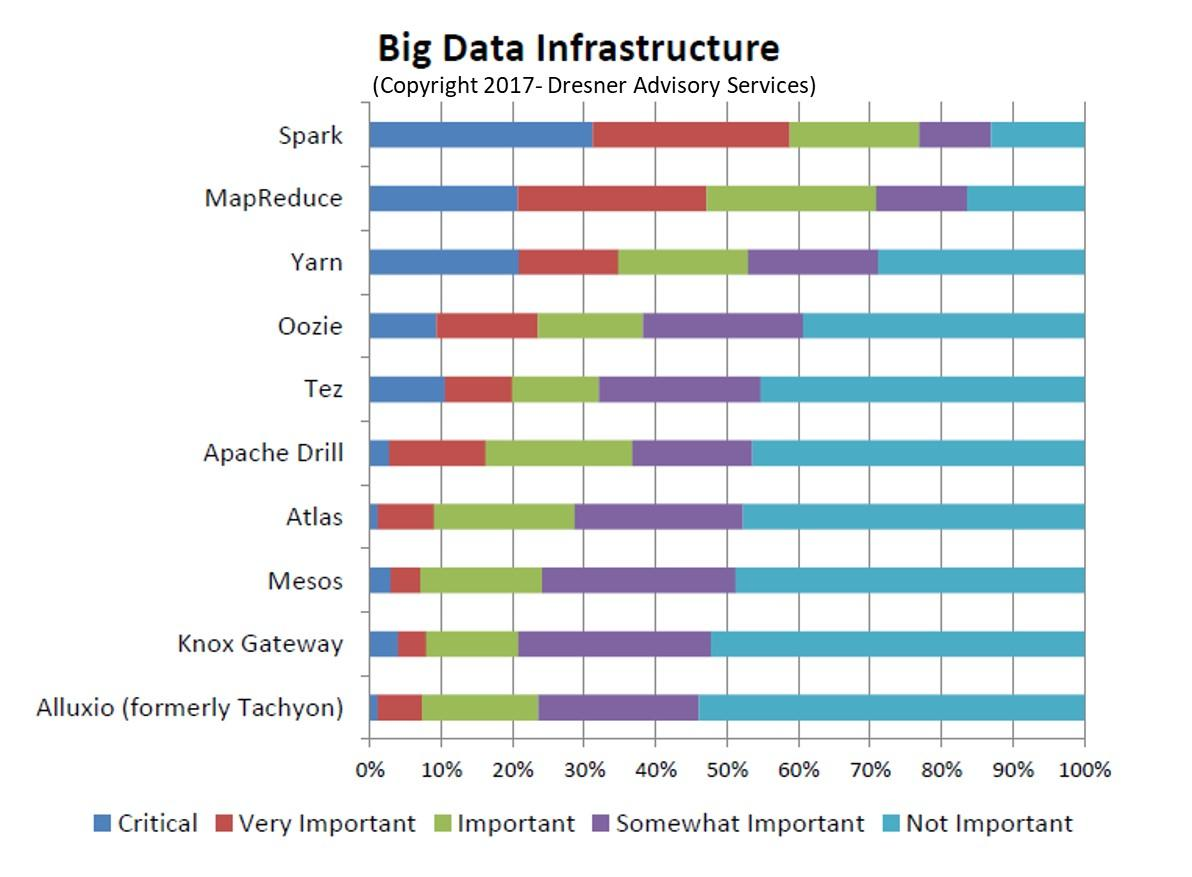
\includegraphics{5.jpg}
\caption{}
\end{figure}

\begin{itemize}
\tightlist
\item
  \textbf{The big data access methods most preferred by respondents
  include Spark SQL, Hive, HDFS and Amazon S3 (Figure 1.6).}
\end{itemize}

\begin{figure}
\centering
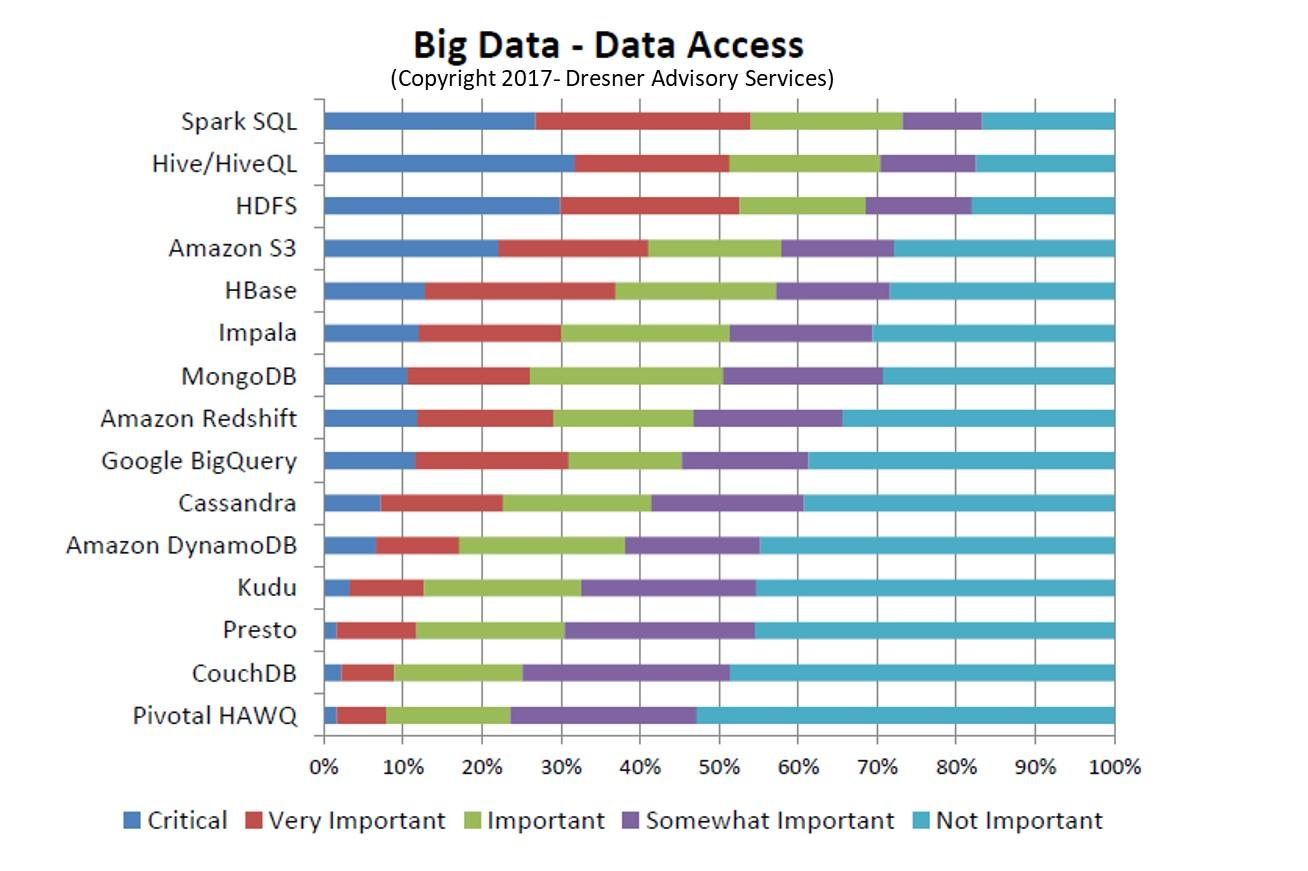
\includegraphics{6.jpg}
\caption{}
\end{figure}

\begin{itemize}
\tightlist
\item
  \textbf{Machine learning continues to gain more industry support and
  investment plans with Spark Machine Learning Library (MLib) adoption
  projected to grow by 60\% in the next 12 months (Figure 1.7).}
\end{itemize}

\begin{figure}
\centering
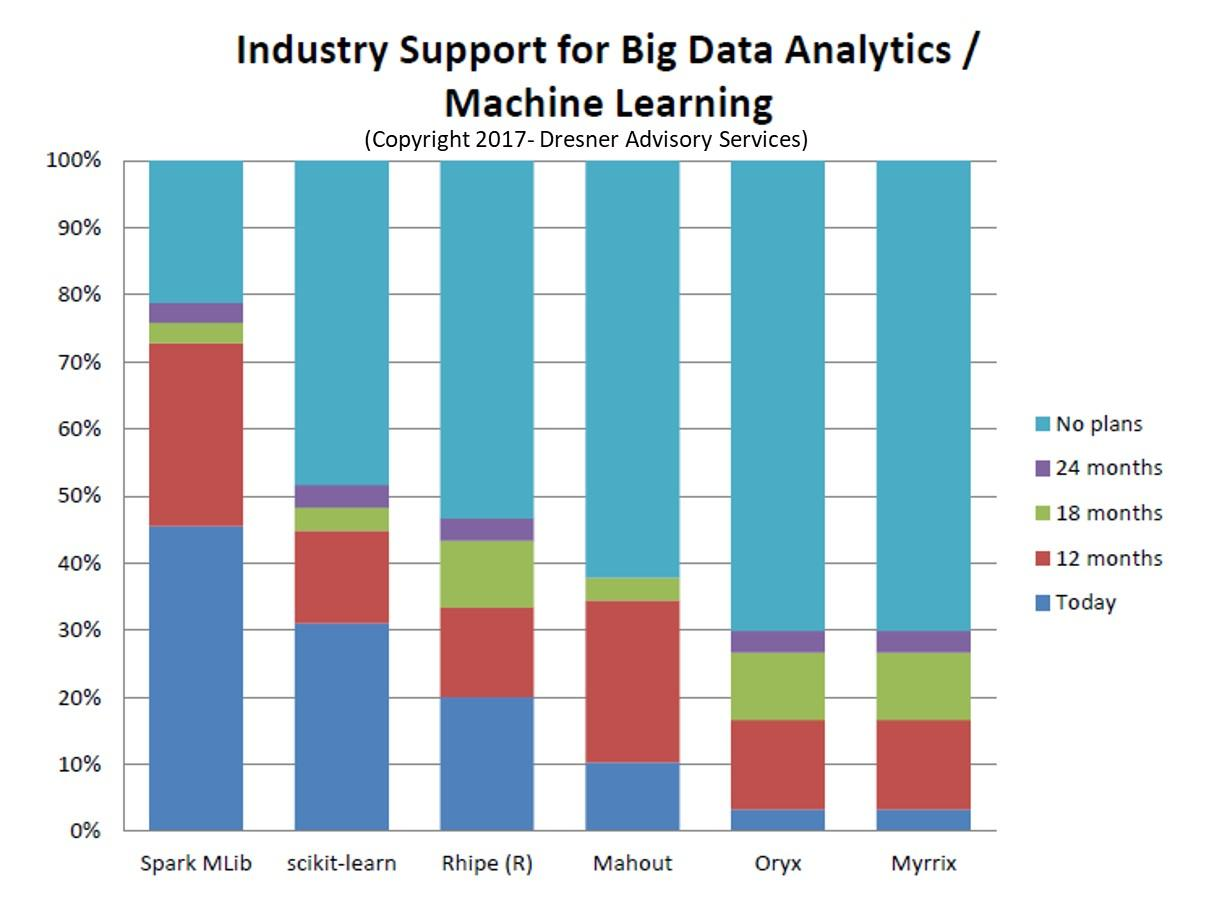
\includegraphics{7.jpg}
\caption{}
\end{figure}

The big four (Deloitte, Ernst \& Young (EY), KPMG and
PricewaterhouseCoopers (PwC)) are the four biggest professional services
networks in the world. They did also so many research about this theme.
One of the interesting information are in the paper ``Gut \& gigabytes''
from PricewaterhouseCoopers (PwC).

The point is that executives rely more on experience and advice than
data to make business-fefining choices but the data driven cultures
could be impact more for decision making.

\textbf{The summary of this paper:}

\begin{quote}
Highly data-driven companies are three times more likely to report
significant improvement in making big decisions, but only 1 in 3
executives say their organisation is highly data-driven.
\end{quote}

\begin{quote}
More big decisions are made opportunistically than deliberately, and big
decisions have big impact on future profitability; nearly 1 in 3
executives value those decisions at \$1 billion+
\end{quote}

\begin{quote}
Many executives sceptical or frustrated by the practical application of
data and analytics for big decisions, especially in emerging markets
\end{quote}

And the five important issues in this survei are growing the existing
business, collaborating with competitors, shrinking the existing
business, entering a new industry or starting a new business, and
corporate financing.

The last questions of this introduction are how data analytics can
improve your businesses? Below are the answered.

\begin{enumerate}
\def\labelenumi{\arabic{enumi}.}
\tightlist
\item
  Make data-driven business decisions
\end{enumerate}

\begin{quote}
Making evidence-based rather than intuition-based decisions
\end{quote}

\begin{enumerate}
\def\labelenumi{\arabic{enumi}.}
\setcounter{enumi}{1}
\tightlist
\item
  Grow your business -- discover new opportunities
\end{enumerate}

\begin{quote}
Quickly identify future markets and the best areas for new investments
Boost growth through strategic pricing models and data-driven marketing
\end{quote}

\begin{enumerate}
\def\labelenumi{\arabic{enumi}.}
\setcounter{enumi}{2}
\tightlist
\item
  Create a more efficient and smarter organization
\end{enumerate}

\begin{quote}
Predict and anticipate the impacts of economic, market, and regulatory
forces on business strategy and results Use automation and advanced
statistical software to handle and analyze huge volumes of data
\end{quote}

\begin{enumerate}
\def\labelenumi{\arabic{enumi}.}
\setcounter{enumi}{3}
\tightlist
\item
  Manage risk and regulatory
\end{enumerate}

\begin{quote}
Minimize compliance risks by ensuring the completeness, accuracy, and
availability of data sources
\end{quote}

\section{Big data definition}\label{big-data-definition}

As data becomes more bigger, manipulating of available data to get
insights and make business decisions can be a useful. Statistical
methods, artificial intelligence, machine learning, and data
manipulation are some of new term that every business leaders at every
level need to become data literate and be able to understand data and
analytical concepts.

Before going further, what is actually Big data?. Big data term comes
from John Mashey in 1990, a computer scientist from Pennsylvania State
University. It all starts with the big bang explosion in the amount of
data we have created since the rise of the digital era. Side effects of
the rise of computers, the Internet and technology that capable of
capturing data from the all kind of electronic processing.

Big Data have 3 defining properties call 3V. This terms introduces by
\texttt{Gartner\ analyst\ Doug\ Laney} in a 2001 MetaGroup research
publication. He publisched that publication with the title ``3D data
management: Controlling data volume, variety and velocity''. Also not
all data is big data except they have 3 properties. Some others data
expert added another 2V, value and veracity, but the main term is always
3V.

\textbf{1. Volume:} Volume refers to the huge amounts of data generated
each time from all of electronics device such as website, social media,
cell phones, cars, credit cards, sensors, photographs, video, etc.
Volume is the V most associated with the term of big data because,
volume can be incredible exploding big. Below is the explanation of how
data growing rapidly from sisense.com (Figure 1.8)

\begin{figure}
\centering

\includegraphics{8.jpg}
\caption{}
\end{figure}

For Example in internet world. Facebook is storing 250 billion images As
far back as 2016, Facebook had 2.5 trillion posts. Can you imagine for
the others online media such as twitter, blog, instagram and also our
searching in google? It is a extreme amount of data. This link show the
live statistics of some online area such as facebook, twitter., internet
users, etc.

\url{http://www.internetlivestats.com/}

(Figure 1.9 and Figure 1.10)

\begin{figure}
\centering
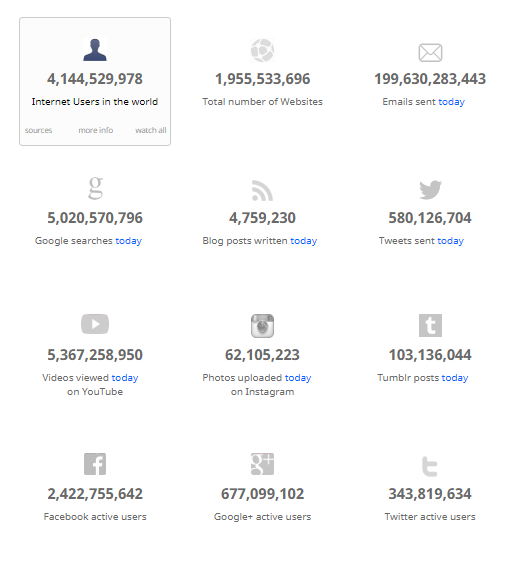
\includegraphics{9.PNG}
\caption{}
\end{figure}

\begin{figure}
\centering
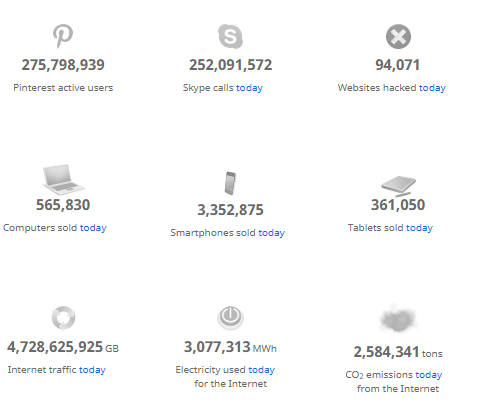
\includegraphics{10.PNG}
\caption{}
\end{figure}

Or

\url{http://www.worldometers.info/}

(Figure 1.11 \& Figure 1.12)

For world parameter infos such as population, health, economics, food,
water, energy, etc.

\begin{figure}
\centering
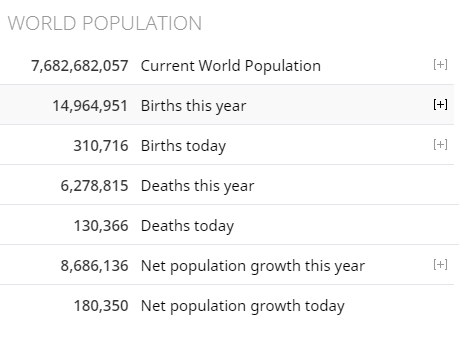
\includegraphics{11.PNG}
\caption{}
\end{figure}

\begin{figure}
\centering
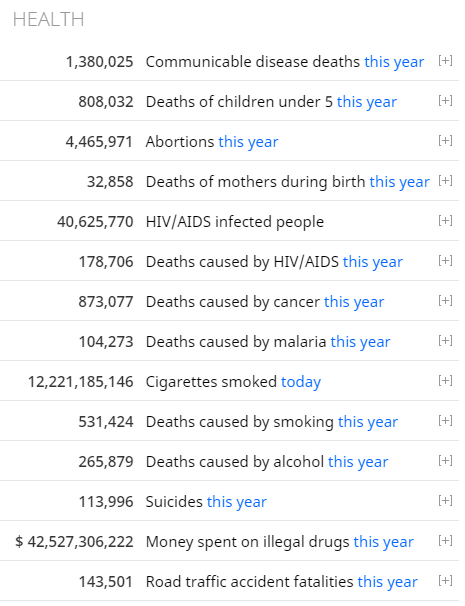
\includegraphics{12.PNG}
\caption{}
\end{figure}

\textbf{2. Variety:} It refers to many sources and data types
(structured and unstructured). Not only spreadsheet and database but
also emails, photos, videos, monitoring devices, audio, etc.

\textbf{3. velocity:} There are four velocity type in big data.

\begin{itemize}
\tightlist
\item
  Batch
\item
  Periodic
\item
  Near real time
\item
  Real time
\end{itemize}

``Firehose'' data sources such as social media and E-commerce need
quickly analytics. Most importantly, use it at a faster rate than ever
before. Using real-time alerting, Walmart company was able to find a
particular Halloween novelty cookie of its stores where it wasn't
selling at all. More than realtime but predictive analytics.

The infographics \& animations to understand more of 3V of big data from
IBM are below (Figure 1.13).

\begin{figure}
\centering
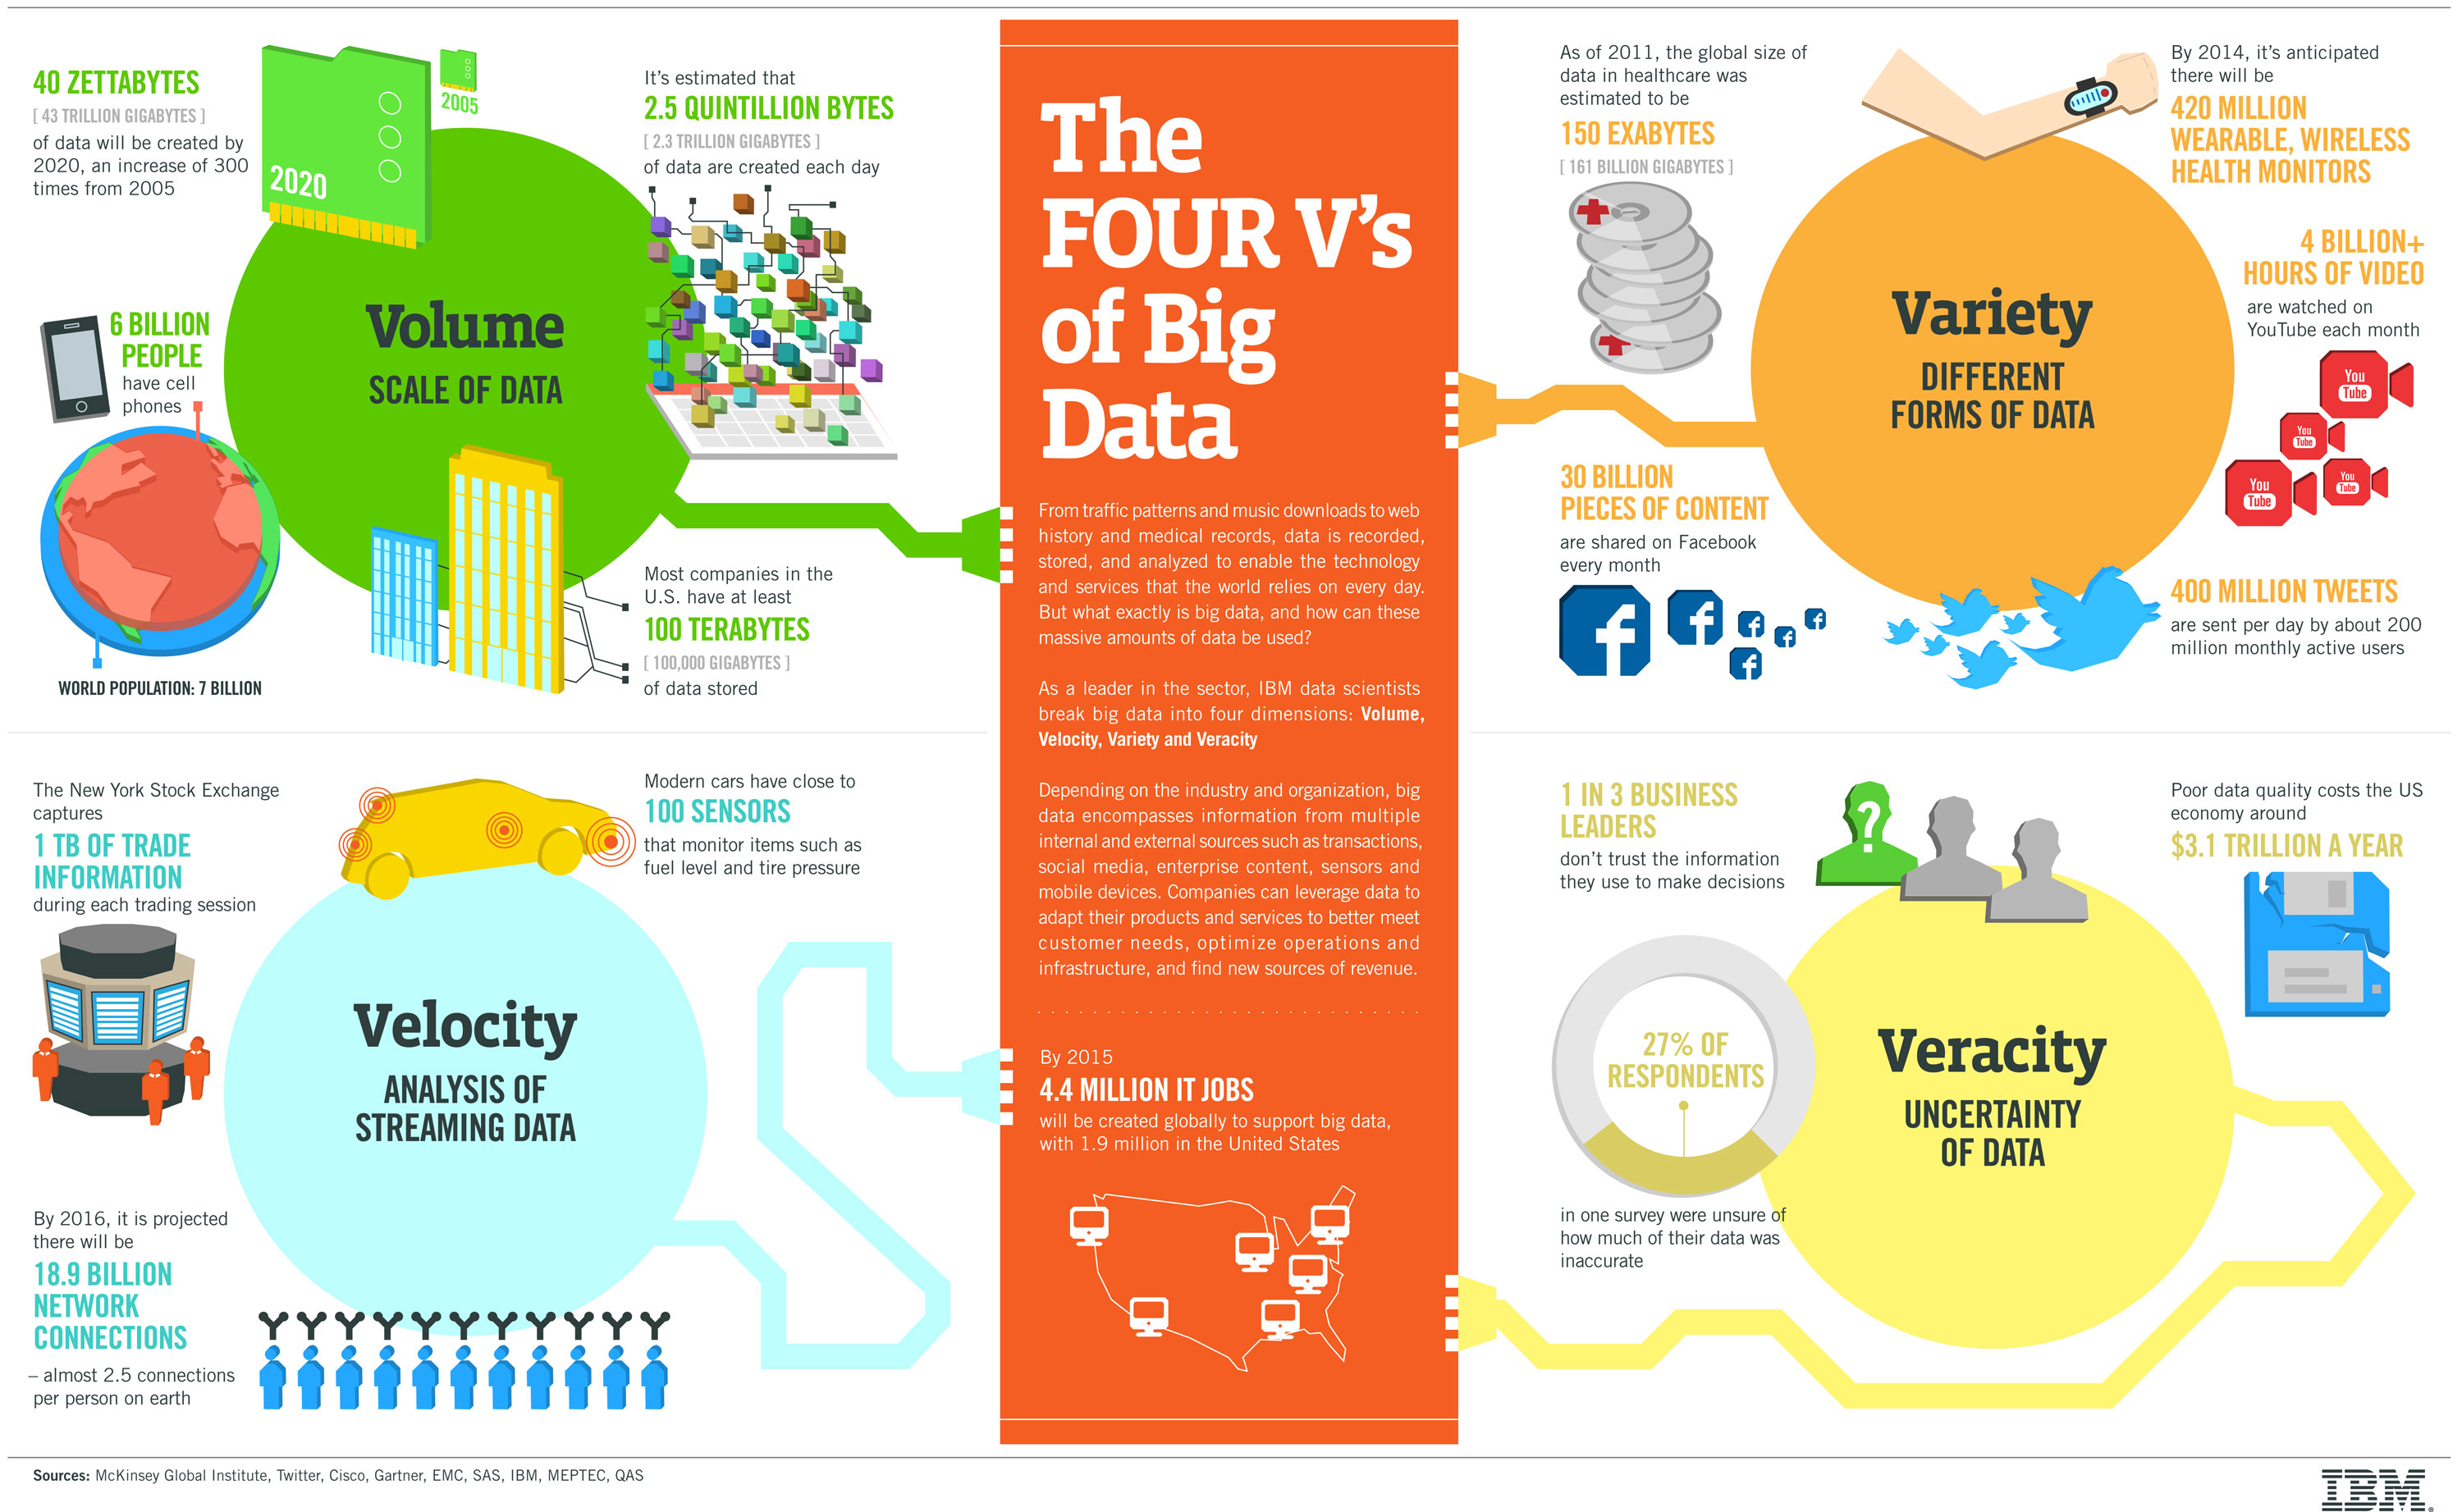
\includegraphics{13.jpg}
\caption{}
\end{figure}

There has been an rapidly growth in the field of Big Data with the
benefits of the rising the new technology. This availability of big data
has led to the use of big data in multiple industries ranging from

\begin{itemize}
\tightlist
\item
  Banking
\item
  Healthcare
\item
  Energy
\item
  Technology
\item
  Consumer
\item
  Manufacturing
\item
  etc
\end{itemize}

The next section are example use case big data in some of industries
(our case studies: transportation and logistics industries and another
industry).

\section{T \& L industry: Deutsche
Bahn}\label{t-l-industry-deutsche-bahn}

Deutsche Bahn AG is a German railway company as the second-largest
transport company in the world, after the German postal and logistics
company Deutsche Post / DHL, and is the largest railway operator and
infrastructure owner in Europe. Headquartered in Berlin, it is a private
joint-stock company (AG), with the Federal Republic of Germany being its
single shareholder.

The Deutsche Bahn Group is divided with some subsidiaries, such as:

\begin{itemize}
\tightlist
\item
  Personenverkehr
\item
  Arriva
\item
  DB Fernverkehr
\item
  DB Regio
\item
  DB Netze
\item
  DB Engineering \& Consulting
\item
  Logistics
\item
  ect
\end{itemize}

\begin{figure}
\centering
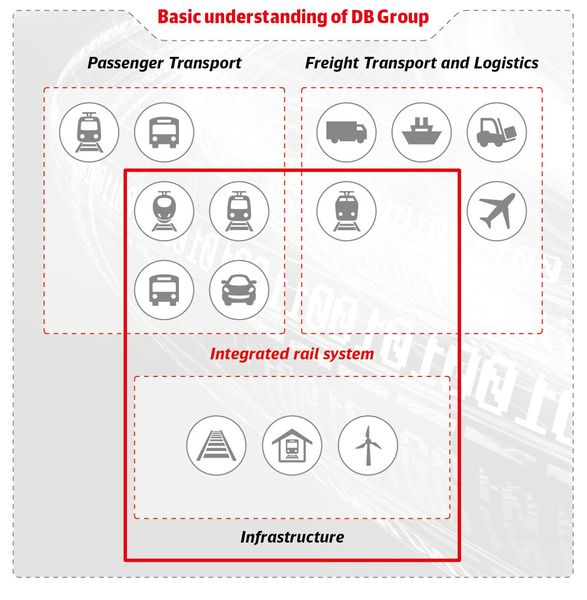
\includegraphics{db.jpg}
\caption{}
\end{figure}

Deutsche Bahn Group (DB Group) is an international provider of mobility
and logistics services operating globally in more than 130 countries. DB
Group has more than 310,000 employees, with almost 40\% employed outside
Germany.

In passenger transport, we transport more than 12.5 million people each
day on our trains and buses throughout Europe. In freight transport and
logistics, our European network transports over 270 million t of goods
per year by rail, and over 100 million shipments by road. Our global
networks move about 1.3 million t of freight by air and nearly 2.2
million TEU by sea. At about 33,000 km, our rail network in Germany is
Europe's longest. We are also the fifth-largest energy provider in
Germany. The main components of our integrated rail system are our
passenger transport activities in Germany, our rail freight transport
activities, the operating service units and the rail infrastructure
companies (RIC).

\begin{figure}
\centering
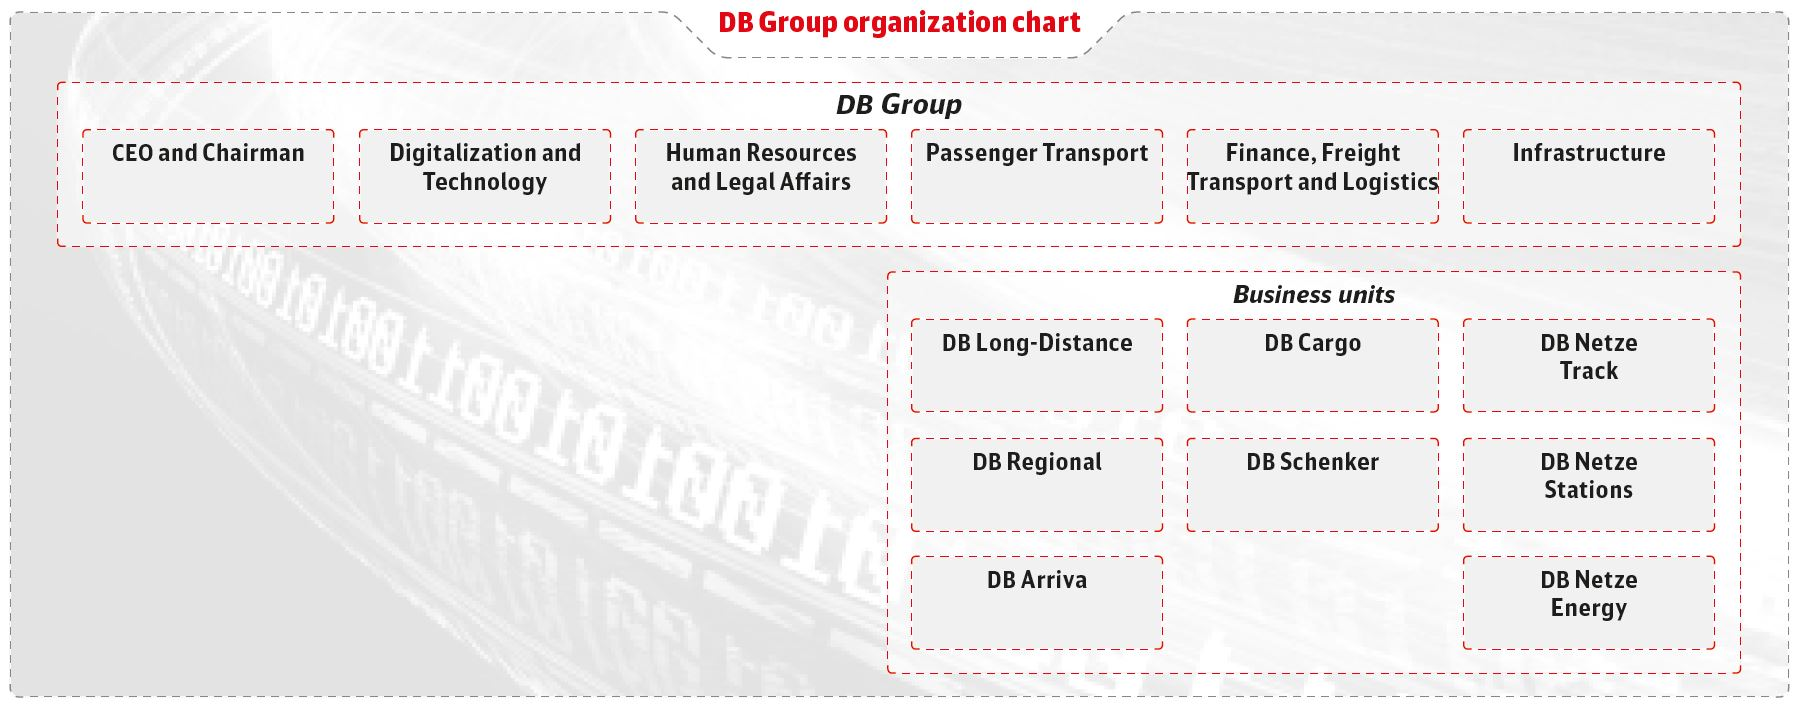
\includegraphics{db2.JPG}
\caption{}
\end{figure}

As an operator of networks and provider of services in passenger
transport, freight transport and logistics, as well as track
infrastructure, our economic success is influenced by the general
economic environment and the specific development of the various
relevant markets.

\begin{figure}
\centering
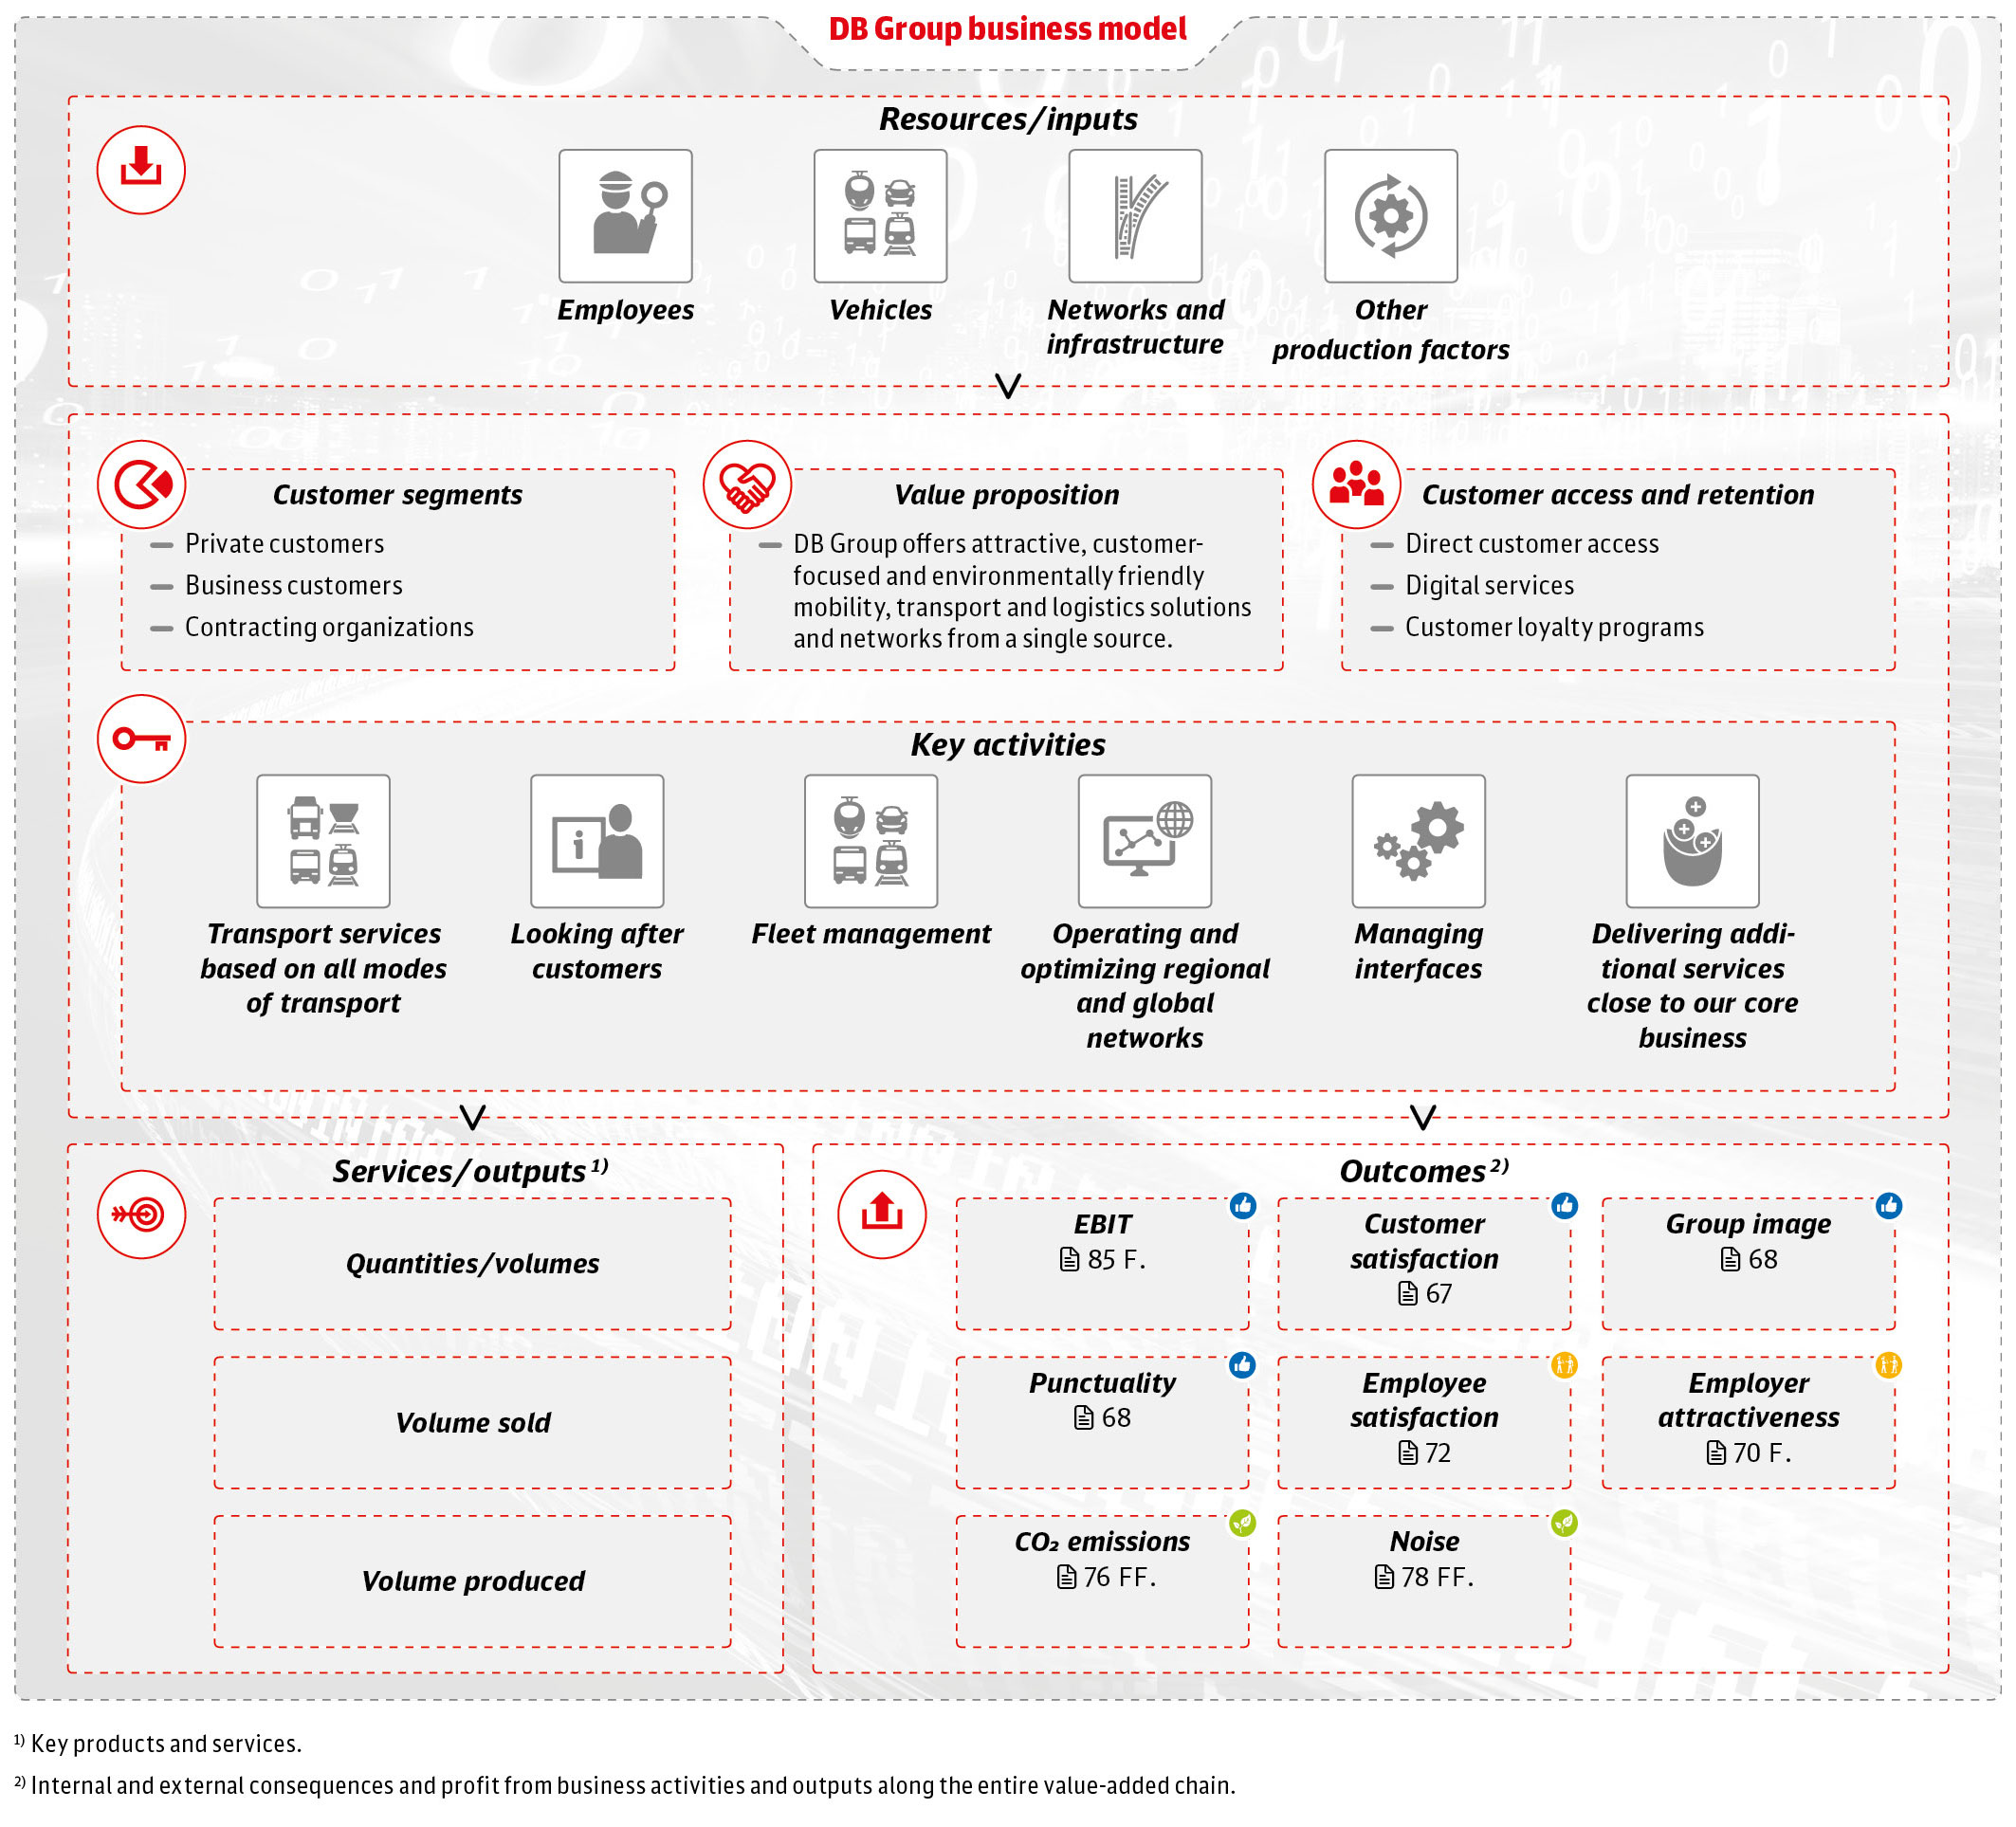
\includegraphics{db3.jpg}
\caption{}
\end{figure}

There are four key success factors in the development of DB Group, which
are a central component of DB Group's business model:

\begin{enumerate}
\def\labelenumi{\arabic{enumi}.}
\item
  Entrepreneurial approach to business: in the course of the German rail
  reform DB Group has established itself as a commercial enterprise.
  Particularly worth mentioning in this context are the establishment of
  a modern and efficient organization and a value-based management
  approach with capital market viability as a target.
\item
  Integrated Group: as a system integrator in Germany, DB Group
  optimizes the integrated rail system. In doing so, it serves as an
  important driving force for technological innovation. The integrated
  Group structure enables us to achieve positive synergies and align our
  infrastructure to support efficiency, market orientation and
  profitability.
\item
  International position: due to our focus on Europe in passenger
  transport as well as our European and global orientation in the areas
  of freight transport and logistics activities, DB Group has an
  excellent position in the relevant markets. As a result, we are
  responding to the increasing demand for cross-border solutions. At the
  same time, we are best positioned to take advantage of growth
  opportunities.
\item
  Cross-modal transport solutions: we offer our customers door-to-door
  mobility and logistics solutions from a single source. We use digital
  technologies to intelligently link various modes of transport in an
  economical and environmentally friendly way. In addition, we offer
  complementary products and services in the freight transport and
  logistics market.
\end{enumerate}

One of the subsidiary company that focusing on big data analytics to
achive that key succes factors is DB Systel Gmbh
(\url{https://www.dbsystel.de/dbsystel}). The key point of DB Systel
are:

\textbf{Big data}

If the data can no longer be stored by conventional databases, it is
known as big data. We need mathematical methods, statistical, machine
learning, and alghorithms to get insigh from the big data.

\textbf{Business intelligence/business analytics}

The process to collected, analysed, and visualized data, either as bar
graph, pie chart or another form. The KPI (Key Performance Indicators)
are the main end results from this process. And support decision making
in the present and also future

\textbf{Data mining}

The three main concepts of data mining are statistics, mathematics, and
alghorithms. To detect the hidden patterns and connections in big data
we need some methods, such as clustering (formation of groups of similar
data), regression analysis (what depends on which other factors?) and
association (if one thing happens, another does too)

\textbf{Data lake}

Every day, individual generates around 650 megabytes of data. There is a
lake of data. Creating the data lake is a logical way of helping company
to get flexible access to all of the data sources. A data lake is a
central location where every department can store external and internal
data (structured and unstructured data at any scale).

\begin{figure}
\centering
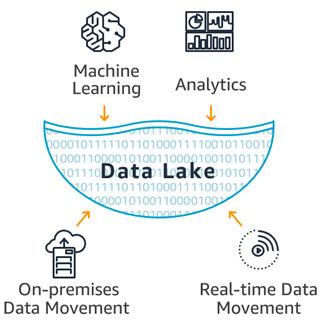
\includegraphics{datalake1.png}
\caption{}
\end{figure}

Data Lakes compared to Data Warehouses.

\begin{figure}
\centering
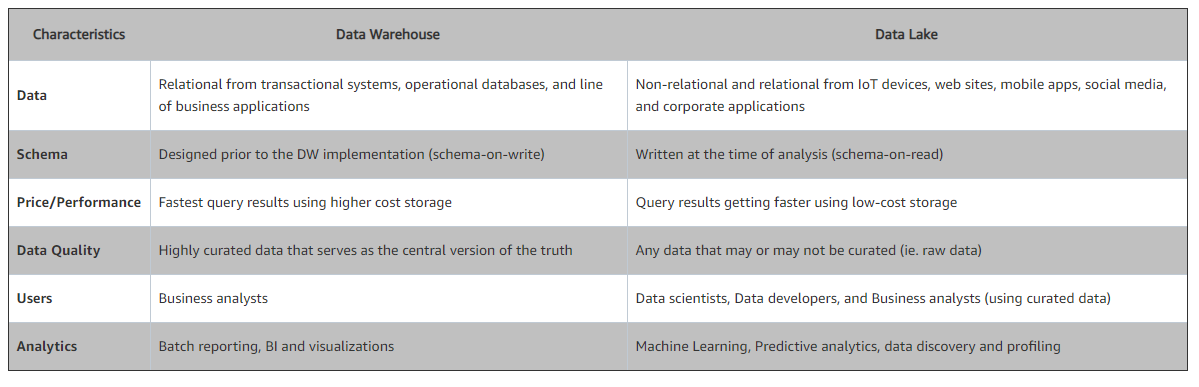
\includegraphics{datalake.PNG}
\caption{}
\end{figure}

\textbf{Smart data}

While big data and the data lake consist of structured data and
unstructured data, smart data have a specific purpose using certain
algorithms and other tools. Smart data developed and improving a
business processes and decision-making. The smart data consist also the
analytics Edge, such as:

\begin{itemize}
\tightlist
\item
  Descriptive analytics
\item
  Predictive analytics
\item
  Prescriptive analytics
\end{itemize}

The description of this three analytics edge you can find in the next
chapter \texttt{3.\ Big\ Data\ Analytics}

\begin{figure}
\centering
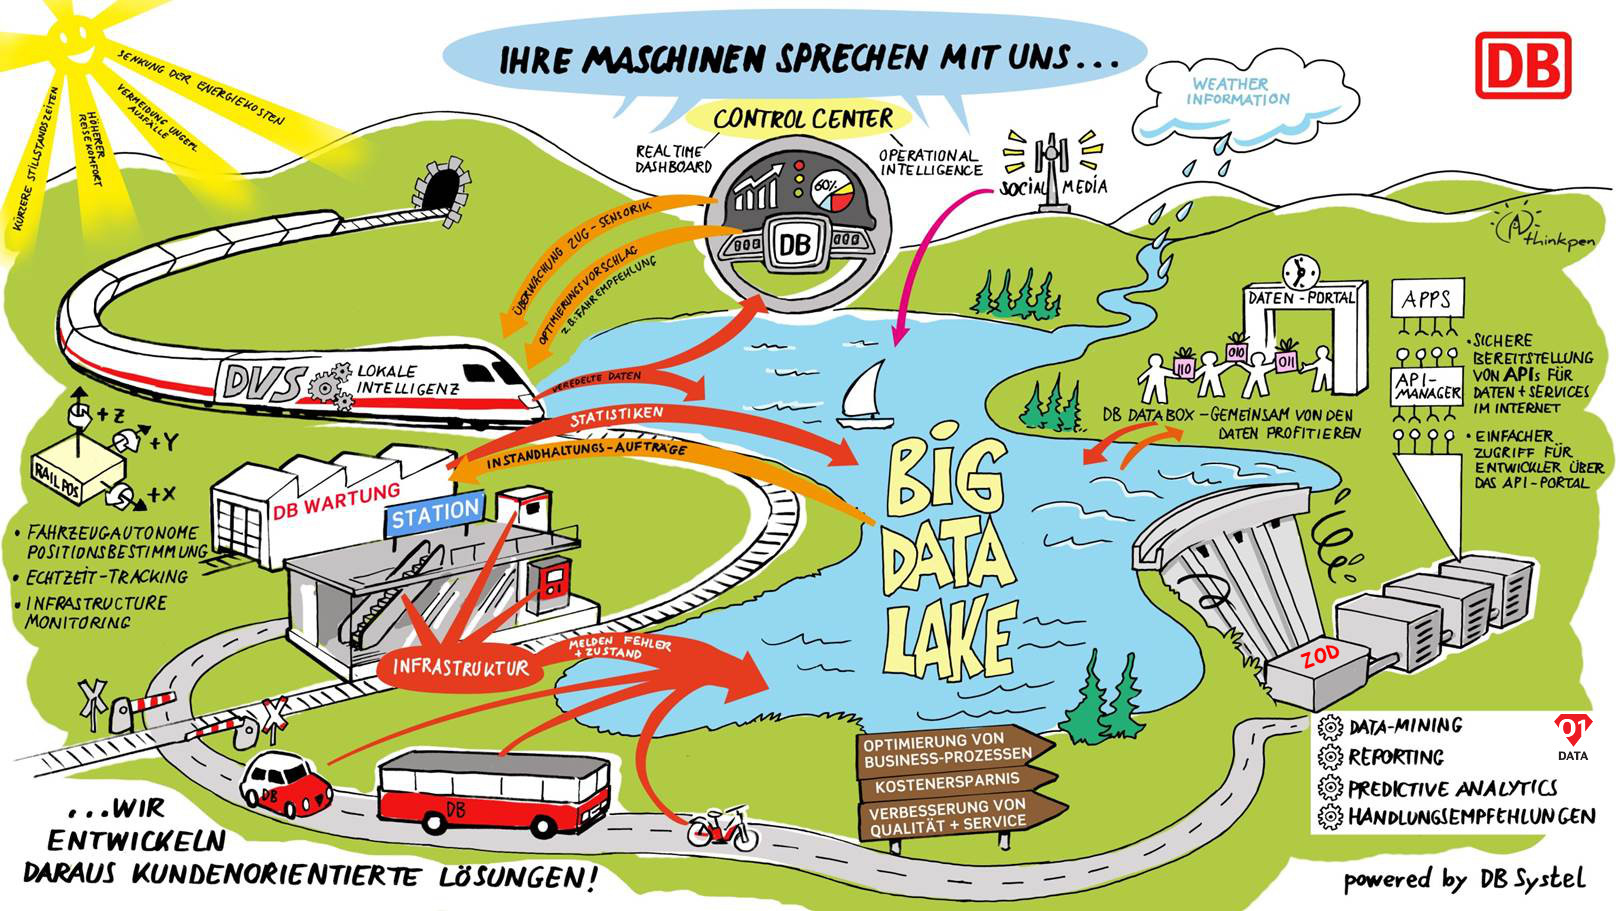
\includegraphics{dbbigdata.jpg}
\caption{}
\end{figure}

Like most other industries, transportation and logistics (T\&L) is
currently confronting immense change and like all change, this brings
both risk and opportunity. This risk and opportunity have new
technology, new market, new customers expectation, and new business
modell. Based on pwc (PricewaterhouseCoopers) research, there are four
disruption and uncertainty and five forces transforming in the era of
big data for T\&L industry (Transportation \& Logistik).

\textbf{Four areas of disruption and uncertainty:}

\begin{enumerate}
\def\labelenumi{\arabic{enumi}.}
\tightlist
\item
  Changing customer expectations
\end{enumerate}

Like individual consumers, industrial customers now expect to get
shipments faster, more flexibly, and with more transparency at a lower
price. No surprise that across the industry, both operating models and
profitability are under strain. And the pace of transformation for large
manufacturing and retail customers may turn out to be even faster than
for private final consumers.

\begin{figure}
\centering
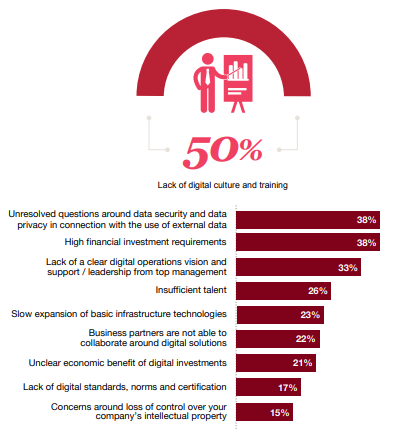
\includegraphics{pwc1.PNG}
\caption{}
\end{figure}

\begin{enumerate}
\def\labelenumi{\arabic{enumi}.}
\setcounter{enumi}{1}
\tightlist
\item
  Technological breakthroughs
\end{enumerate}

Technology is changing every aspect of how logistics companies operate.
`Digital fitness' will be a prerequisite for success: the winners will
be those who understand how to exploit a whole range of new
technologies, from data analytics to automation and platform solutions.
Those who don't, risk obsolescence. But with so many technologies
competing for management attention and investment, defining a clear
digital strategy that's integrated into business strategy will be
critical.

\begin{figure}
\centering
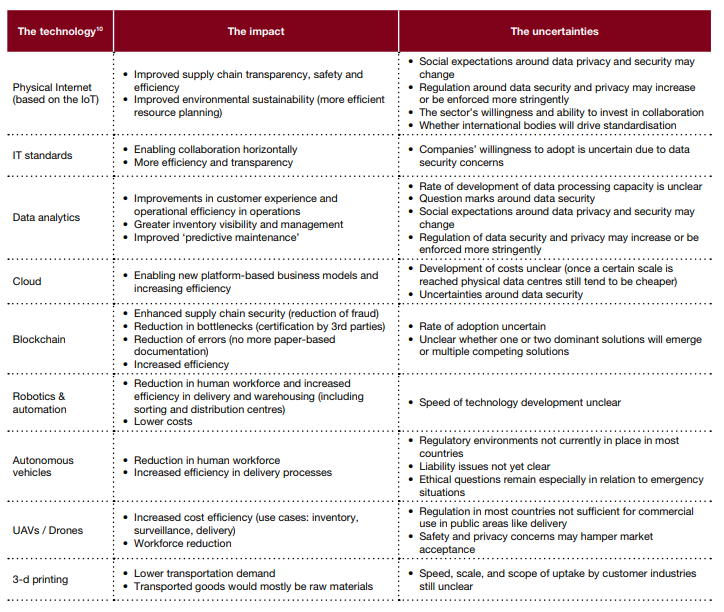
\includegraphics{pwc2.PNG}
\caption{}
\end{figure}

\begin{enumerate}
\def\labelenumi{\arabic{enumi}.}
\setcounter{enumi}{2}
\tightlist
\item
  New entrants to the industry
\end{enumerate}

Platform technology has given rise to new business models, often driven
by start-ups that enter the logistics industry. New `sharing' business
models could have as much of an impact on the sector as new technology.
And the industry's current customers and suppliers may end up being the
biggest new entrants.

\begin{enumerate}
\def\labelenumi{\arabic{enumi}.}
\setcounter{enumi}{3}
\tightlist
\item
  Redefining collaboration
\end{enumerate}

Horizontal collaboration is already happening, especially in last-mile
delivery, but it's hampered by inconsistencies. Higher levels of
efficiency could be achieved by more consistent standards, defined
through the Physical Internet and increased collaboration, whether in
the form of alliances, joint ventures or M\&A.

\textbf{Five Forces Transforming Transport \& Logistics:}

As the complexity of modern transport and logistics grows, it is
increasingly difficult to understand what to focus on, so PWC have
identified five key forces transforming the T\&L segment:

\begin{enumerate}
\def\labelenumi{\arabic{enumi}.}
\tightlist
\item
  Digitalization
\item
  Shifts in international trade
\item
  Software-driven process changes
\item
  Changes in markets' domestic commerce
\item
  Machine-driven process changes
\end{enumerate}

\begin{figure}
\centering
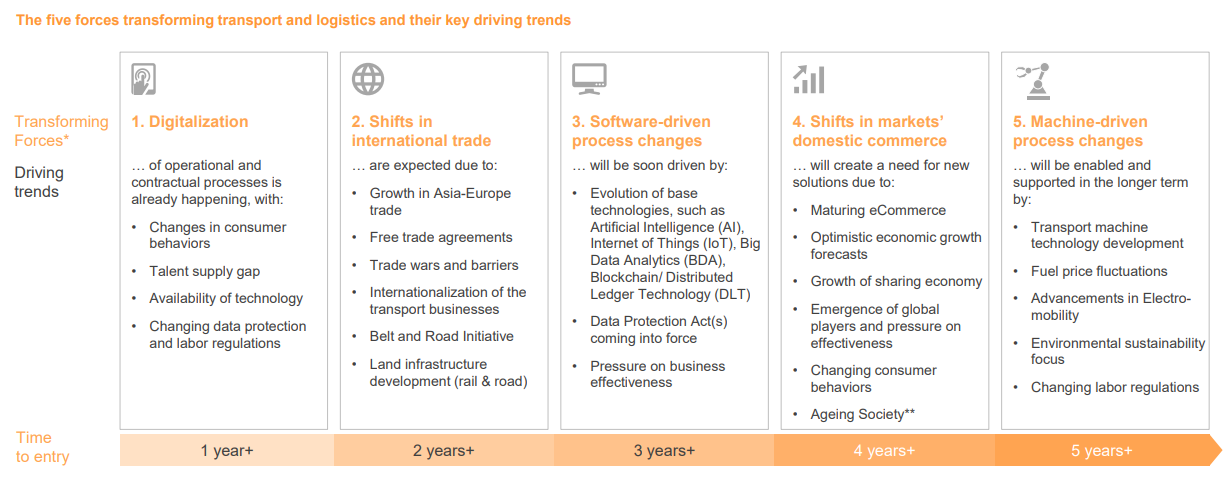
\includegraphics{pwc3.PNG}
\caption{}
\end{figure}

\section{Another industry}\label{another-industry}

\subsection{Agriculture}\label{agriculture}

Agriculture businesses are using big data to improve production and
yields and improve forecasting to better optimize supply chains. Getting
deep insight through big data is important to highing product quality or
rising sales and market share.

As agribusinesses growth and more diverse, the growing of data that must
be managed are also becoming more huge and complex. The data comes from
not only social media outlets and supplier network channels but also
agricultural devices sensor and machine equipment. Today these data
sources come from:

\begin{itemize}
\tightlist
\item
  Traditional enterprise data from operational systems
\item
  Farm field sensor data (e.g.~temperature, humidity, rainfall,
  sunlight)
\item
  Farm equipment sensor data (from tractors, plows, and harvesters)
\item
  Harvested goods and livestock delivery vehicles (from farms to
  processing facilities) sensor data
\item
  Commodities trade data
\item
  Financial data
\item
  Weather data
\item
  Animal and plant genomics research data
\item
  Social media
\end{itemize}

Big Data can help improve forecasting and efficiency and lead precisely
decision making. Big data technologies enable agricultural sectors to
analyze a variety of data sources, in turn leading to better outcomes.
Agribusinesses have long lists of needed metrics. But which data that we
need and where the data come from and also what is the outcome or
beneficially result. Following is a list of areas where Big Data
technologies can impact in agricultural sectors:

\begin{itemize}
\tightlist
\item
  Weather data from weather institution for better understanding time to
  plants
\item
  Improved forecasting of yields and production data from Farm field
  sensor data (e.g. temperature, humidity, rainfall, sunlight)
\item
  Better optimized seeds and livestock and new methodologies that
  improve yields and production with Farm equipment sensor data such as
  warehouse sensor data
\item
  Faster delivery of goods produced to distribution centers and
  consumers with street data or vehicle (car) sensor data
\item
  Real-time decisions and alerts based on data from fields and equipment
  with Farm equipment sensor data or Farm field sensor data
\item
  Integrated production and business performance data for improved
  decision making with ERP system from integrated all sensor devices and
  sales data.
\item
  Rationalized performance data across multiple geographies with sales
  data
\item
  Accurate crop predictions with weather and crop data
\item
  Stronger seeds and less hunger with plant data with purpose developing
  crops that can grow in any environment -Automated agriculture for
  better production with different system
\end{itemize}

\begin{figure}
\centering
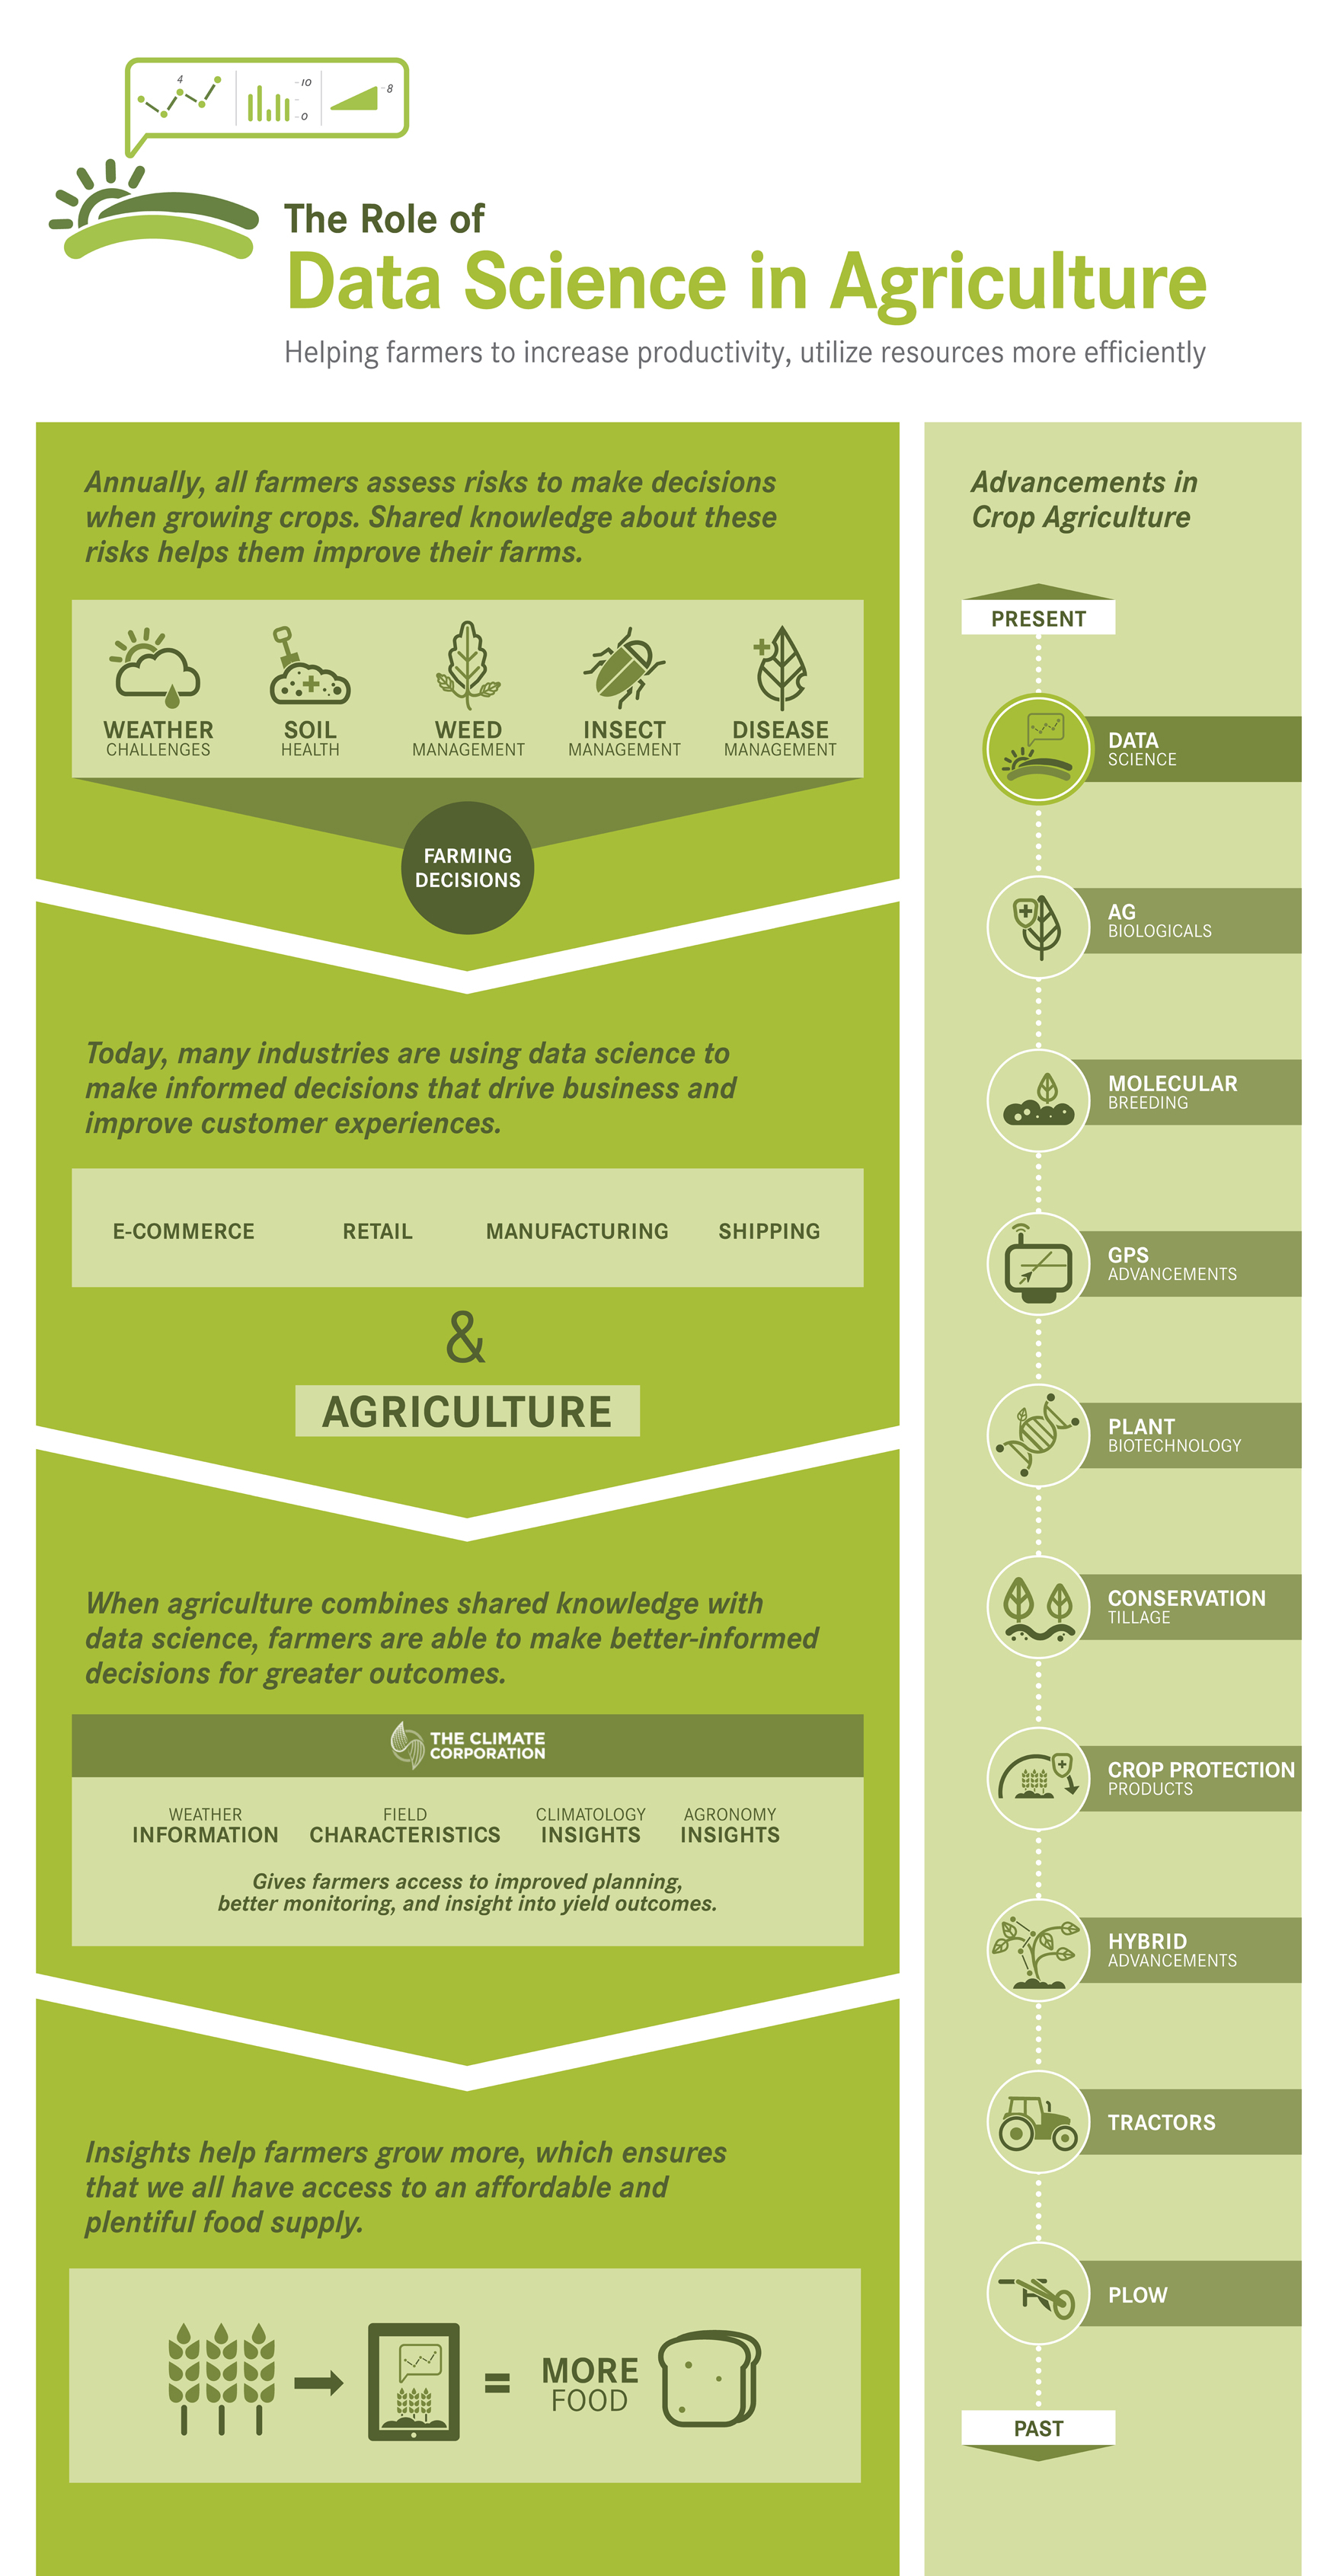
\includegraphics{14.jpg}
\caption{}
\end{figure}

\subsection{Automotive}\label{automotive}

The automotive industry face a compleks challenges. One thing that has
the opportunity to deliver solution is analytics. Shifting marketing
conditions, volatility, competition, and cost pressure are the problem
to change in the automotive industry.

As the automobile is being transformed by big data technologies
(everything from sensors to artifical intelligence to big data
analysis). The ecosystem are change and the analytics allows the data
not only structured but also unstructured data such as videos, sound
recording, or texts to be analyze- the results are impressive.

\begin{figure}
\centering
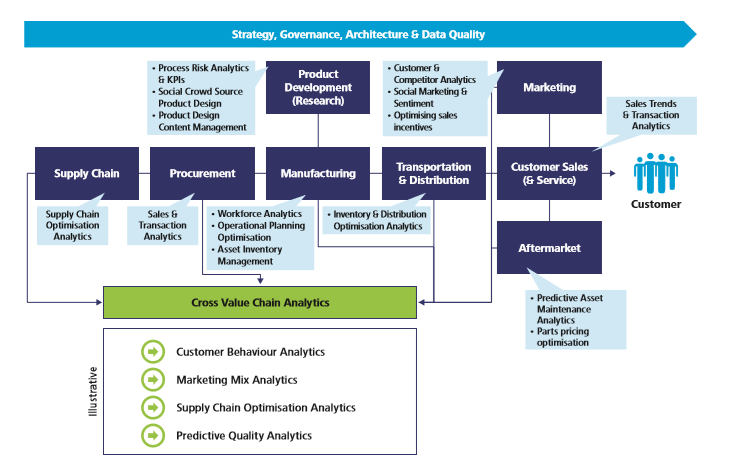
\includegraphics{15.png}
\caption{}
\end{figure}

Below are the key points to deep undestand the automative industry:

\begin{itemize}
\tightlist
\item
  \textbf{Use the data for actionable customer segments and
  individualised offers and to boost sales and also improve customer
  retention.}
\end{itemize}

Customer behaviour analytics: Customer need a consistent personalised
experience across their access channels.Automakers are having to sell by
offering 24/7 connectivity and reliance on social media and internet as
communication tool. There is a huge of data available to support
automakers for understand their customers but automakers have limits and
ability to collect, analyse, and act on it.

Automakers need to fully understand customers needs and behaviours to
develop a bird view of customer segmentation. For example, the
combination of online retailing and physical stores to build brand
awareness, attract new target and transformational retailing experience
for shopping anytime and anywhere. At least but not last, customer
retention needs to be placed high on the strategy, understanding the
customer experience with the lifecycle and journey not only just during
the purchase.

The example of real strategy:

\begin{quote}
Inner city mobility: Pay for use customer mobility solution, covering
central city locations, offering ease, speed and flexibility of commute
\end{quote}

\begin{quote}
Urban lifestyle convenience: Taking direct retailing and servicing
business to the consumer
\end{quote}

\begin{quote}
Regional retailing: Providing the complete digitised brand experience
through existing dealers
\end{quote}

\begin{itemize}
\tightlist
\item
  \textbf{Applying big data analysis to a mass historical data to
  identify the impact of fixed and variable marketing parameters and
  suppport auto industry with a more precise and effective approach to
  quantity and composition of marketing cost.}
\end{itemize}

The growth in data and information available on customers is allowing
automakers and dealers to focus on spesific customers. To make this
happens, automakers bring togethers internal and external information
sources relating to variable marketing spend to better undestand what`s
working and what isn´t. Besides that, there are some issue that must be
overcome, including:

\begin{quote}
Lack of available data on transaction for internal and competitor
brands.
\end{quote}

\begin{quote}
Less understanding of competitor marketing and strategies
\end{quote}

\begin{quote}
Differences in customer behaviours across different region and customer
segments
\end{quote}

\begin{quote}
Less ability to understand the impact of trends on market and buying
behaviours
\end{quote}

\begin{itemize}
\tightlist
\item
  \textbf{Supply chain data can reveal which links in chain could weaken
  allowing for proactive and timely countermeasure before real problem
  manifests.}
\end{itemize}

Globalising operations to take adventage of high-growth markets, driving
innovative strategies to optimise manufacturing process. Get it right
and gain a competitive advantage and drive growth. Get it wrong and
automakers can get difficult scenarios from parts shortages, government
security, or lost growth opportunities. Moreover, advanced suppy chain
analytics can help automakers analyse larget dataset using analytical
and mathematical techniques. An example of this is the use of product
configuration and web interactions which allow automakers to get early
of emerging trends and forecast.

\begin{itemize}
\tightlist
\item
  \textbf{Predictive analytics for forecasting efficiency as well as
  operations and performance.}
\end{itemize}

The good news is that predictive quality analytics capabilities
available today allow quality issues to be detected and taken prevented.
This news provided improved ability to better manager customer
satisfaction and cost control concerns.

\subsection{Retail}\label{retail}

\begin{figure}
\centering
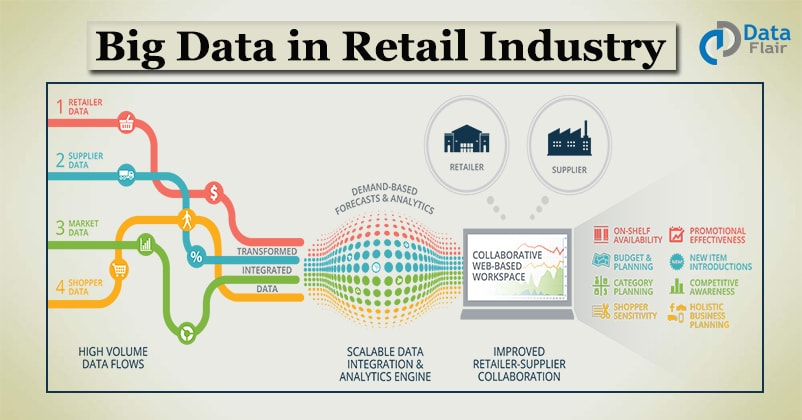
\includegraphics{16.jpg}
\caption{}
\end{figure}

The sphere of the retail industry develop rapidly. Besides that, retail
industry is the top use case of big data. The retailers manage to
analyze data from different sources and develop overview of a customer
to learn targeting sales. Besides that, a customer need to be easily
influenced by the strategy develop by another retailer. New sources of
data, from machine data (log files) and transaction, to sensor and
social media, present opportunities for retailers to get impacted value
and competitive advanced. To achieve this is to make best plans and
decisions, undertand customer more deeply, uncover hidden trends, and
becoming data driven organisation.

This examples presents top big data analytics use cases in the retail,
created for retailers to be aware about trends and tendencies using big
data.

\begin{enumerate}
\def\labelenumi{\arabic{enumi}.}
\item
  Customer Behavior Analytics for Retail: Retailers can combine,
  integrate and analyze all of your external and internal data to
  generate the deeply or hidden insights.
\item
  Customer Journey Analytics: Today's customers are more connected than
  before. Using mobile devices, social media and e-commerce, customers
  can access all of information in seconds. With big data technologies,
  retailers can bring data into powerful insights. Retailers will be
  able to get deeply understanding this questions such as:
\end{enumerate}

\begin{itemize}
\tightlist
\item
  What is s really happening across every step in the customer journey?
\item
  Who are your high-value customers and how they behave?
\item
  How and when is it best to reach them?
\end{itemize}

\begin{enumerate}
\def\labelenumi{\arabic{enumi}.}
\setcounter{enumi}{2}
\tightlist
\item
  Personalizing the In-Store Experience With Big Data
\end{enumerate}

Big data analytics can turn data sources into advantage for retailers.
These data sources can be gathered from:

\begin{itemize}
\tightlist
\item
  Websites
\item
  Point of sales systems
\item
  Mobile apps
\item
  Supply chain systems
\item
  In store sensors
\item
  Cameras and more
\end{itemize}

\begin{enumerate}
\def\labelenumi{\arabic{enumi}.}
\setcounter{enumi}{3}
\tightlist
\item
  Increasing conversion rates through predictive analytics and targeted
  promotions
\end{enumerate}

To reduce costs and high customer acquisition, retailers need targeting
promotions. This requires a 360-degree view of customers situation.

In the past, customer infromation has been limited to demographic data
during sales transactions. But today, customers interact more than they
transact, as example is social media. Using data from internal or
external sources, omni-channel retailers can:

\begin{itemize}
\tightlist
\item
  Test and quantify the impact of different promotional tactics on
  customer behavior and conversion
\item
  Use a customer purchase and browsing history to identify needs and
  interests and then personalize promotions for customers
\item
  Monitor customer purchasing behavior and social media activity to
  drive timely offers to customers to incent online purchases with a
  specific retailer
\end{itemize}

\begin{enumerate}
\def\labelenumi{\arabic{enumi}.}
\setcounter{enumi}{4}
\tightlist
\item
  Recommendation engines
\end{enumerate}

\begin{figure}
\centering

\includegraphics{17.jpg}
\caption{}
\end{figure}

Recommendation engines is one of tools for customers behaviour
prediction. Recommendation engines provided retailers to increase sales
and to dictate trends. Recommendation engines depend on the choices by
the customers. Usually, this engines use either collaborative filtering
or content based recommendation.

\begin{itemize}
\tightlist
\item
  Collaborative Filtering:
\end{itemize}

\begin{figure}
\centering
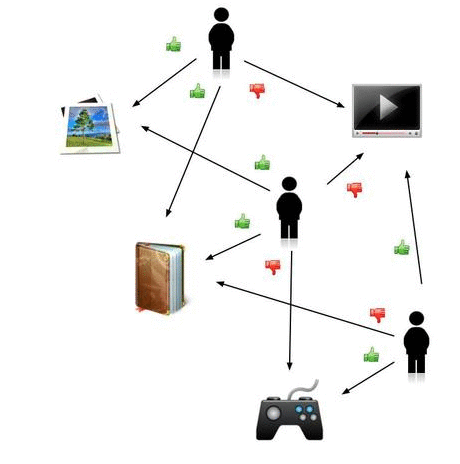
\includegraphics{A.PNG}
\caption{}
\end{figure}

This system based on how similar users liked the item. As example, Cevi
and Herdian have similar interests in games. Cevi buyed and played
``Game of Thrones 4''. Herdia has not played this game. But the system
recommend this game because the system has learned that Cevi and Herdian
have similar interests. In simple words, users who liked this game also
like too.

\begin{itemize}
\tightlist
\item
  Content-based Recommendations:
\end{itemize}

\begin{figure}
\centering
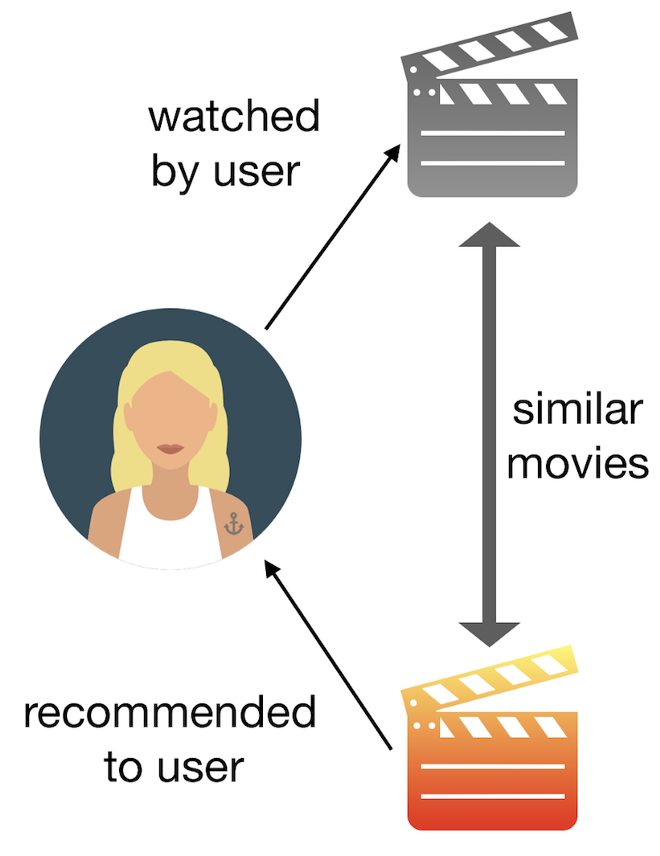
\includegraphics{18.png}
\caption{}
\end{figure}

The company must have detailed metadata (details data explanation about
the data) about each of buyers. Retailers can recommend buyers with
similar tags. For example, Fathimah watch the movies ``Game of Thrones
1'' on Netflix. This movie may have metadata tags of ``War'', so Netflix
recommends to Fathimah another movis with metadata tags ``Ancient''.

\begin{enumerate}
\def\labelenumi{\arabic{enumi}.}
\setcounter{enumi}{5}
\tightlist
\item
  Market basket analysis (transaction data)
\end{enumerate}

Market basket analysis may be regarded as traditional analysis in the
retail. This it a modelling method based on the theory that you buy a
certain items, you are more (or less) to buy another items. This process
mainly depend on the amount of data collected via customers
transactions. It works by looking for combinations of items in
transactions. Association Rules are widely used to analyze retail basket
or transaction data. An example of step by step Association Rules are:

\begin{itemize}
\tightlist
\item
  Assume there are 1000 customers
\item
  100 of them bought only CD games, 850 bought Playstation and 50 bought
  both of them.
\item
  Bought CD games =\textgreater{} bought playstation
\item
  Support = P(CD games \& Playstation) = 50/1000 = 0.05
\item
  Confidence = support/P(Playstation) = 0.05/(850/1000) = 0.05/0.85=0.06
\item
  Lift = confidence/P(Milk) = 0.75/0.10 = 7.5
\end{itemize}

Note:

\begin{quote}
Support:= the number of transactions that include items in the \{A\} and
\{B\} parts of the rule as a percentage of the total number of
transactions.
\end{quote}

\begin{quote}
Confidence:= the ratio of the number of transactions that include all
items in \{B\} as well as the number of transactions that include all
items in \{A\} to the number of transactions that include all items in
\{A\}
\end{quote}

\begin{quote}
lift:= the ratio of confidence to expected confidence. Expected
confidence is the confidence divided by the frequency of B
\end{quote}

\begin{enumerate}
\def\labelenumi{\arabic{enumi}.}
\setcounter{enumi}{6}
\tightlist
\item
  Fraud detection
\end{enumerate}

\begin{figure}
\centering
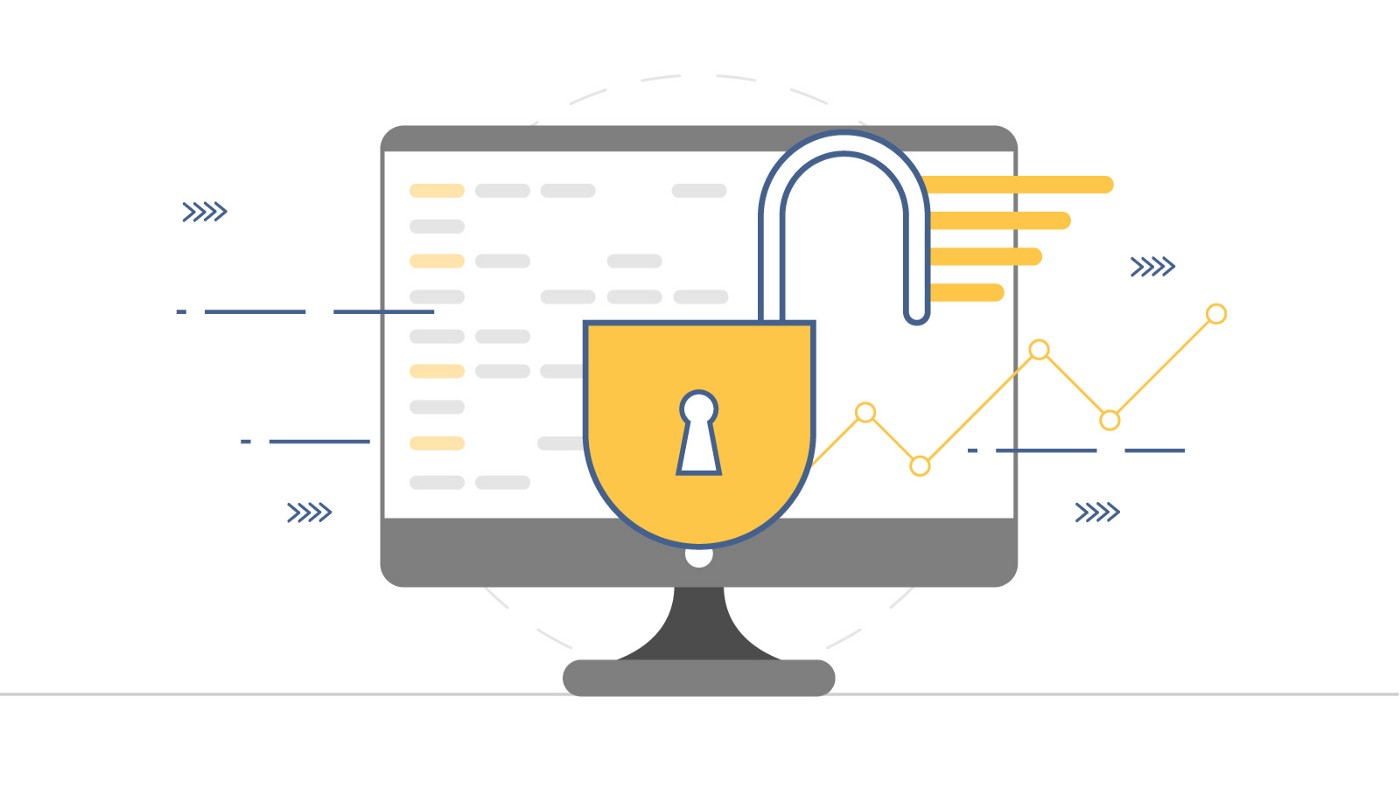
\includegraphics{19.jpg}
\caption{}
\end{figure}

Fraud can encompass abuse and wate, improper payments money laundring,
terrorist financing, cybersecurity and public security. The detection of
fraud is important and challenging activity of retailers. The only good
way to protect retailers is to be one step ahead of fraudsters.

To identify of fraud-while improving customers experienceces-retailers
should follow four steps:

\begin{enumerate}
\def\labelenumi{\arabic{enumi}.}
\item
  Extract and transform all available data types from across departments
  or channels and incorporate them into the analytical process.
\item
  Continually monitor transactions, social networks, high-risk
  anomalies, etc., and apply behavioral analytics to enable real-time
  decision making.
\item
  Intstall analytics culture through data visualization at all levels,
  including investigative workflow optimization.
\item
  Employ layered security techniques (another company who experts in
  this area).
\item
  Warranty analytics
\end{enumerate}

With warranty issues costing retailers billions and indirect cost
factors. To reduce warranty costs, build loyalty customer service, smart
manufactures, and focus on post-sales service. The methods of detecting
are complicated. They concentrate on the detecting anomalies in the
warranty claims.

The warranty analytics have some of challenges:

\begin{itemize}
\tightlist
\item
  Increasing warranty costs and poor customer satisfaction ratings.
\item
  Cannot track warranty claims and resolutions in a timely manner.
\item
  New issues grow in the field for months before they are detected.
\item
  Hard to integrate and analyze historical/supplier warranty
  information, so it is difficult to anticipate and prepare for future
  issues.
\item
  Business analysts and executives do not have ready access to warranty
  data and reports.
\item
  Difficulty integrating quality and warranty data.
\item
  Root cause analysis takes too long.
\item
  Feeding warranty claim information back to design and manufacturing
  takes too long.
\item
  Ineffective, manually intensive processes.
\end{itemize}

\begin{enumerate}
\def\labelenumi{\arabic{enumi}.}
\setcounter{enumi}{8}
\tightlist
\item
  Customer sentiment analysis
\end{enumerate}

\begin{figure}
\centering

\includegraphics{20.jpg}
\caption{}
\end{figure}

Social networks (social media) and online services feedbacks can perform
the sentiment analysis. Because social media data are available,also
much easier to implement analytics on social platforms. This analysis
uses language processing to know a positive ot negative attitude of
customer. The results are as a insight fro services improvement.

The examples are:

\begin{itemize}
\tightlist
\item
  I do not dislike this games. (Negation handling)
\item
  Disliking a games is not really my thing. (Negation, inverted word
  order)
\item
  Sometimes I really hate the Gun. (Adverbial modifies the sentiment)
\item
  I'd really truly love going out in this weather! (Possibly sarcastic)
\end{itemize}

\begin{enumerate}
\def\labelenumi{\arabic{enumi}.}
\setcounter{enumi}{9}
\tightlist
\item
  Price optimization
\end{enumerate}

Pricing optimization is the setting a price to maximize profits. It is
driven by the supply and demand data, behavioural data, competition
data,etc. The right price for customers and retailers is significant
advantage brought by optimization method. The price depends not only on
the costs to produce but on the the competition. The big data analysis
bring this issue to the next level. The data come from many sources and
define buying attitude, seasoning, competitor pricing, etc. The
alghorithm define the response the changes in prices. Using the real
time optimization the retaliers have an advantage to attract more
customers and to build personal pricing schemes.

Below are overview four 6 pricing strategies with big data:

\begin{quote}
\begin{enumerate}
\def\labelenumi{\arabic{enumi}.}
\tightlist
\item
  Premium pricing: Retailers set costs higher than their competitors
  with premium services or items.
\item
  Pricing for Market Penetration: Retailers offer lower prices on goods
  and services for first time opened.
\item
  Bundle Pricing: Buy 1 get 1 pricing.
\item
  Psychology Pricing: For example, setting the price of a watch at \$499
  is proven to attract more consumers than setting it at \$500.
\item
  Price Skimming: The retaliers offer lowers prices as competitor goods
  appear on the market not only for the first time opened.
\item
  Economy Pricing: An example of economy pricing is generic food sold at
  grocery stores. The generic They need little marketing and promotion
  expenses.is incredibly effective for large retailers companies.
\end{enumerate}
\end{quote}

\begin{enumerate}
\def\labelenumi{\arabic{enumi}.}
\setcounter{enumi}{10}
\tightlist
\item
  Location of new stores
\end{enumerate}

Data analytics is efficient about this issue. The method is simple and
also useful. The data are customers data, ZIP code and location for
understanding the market potential. The Analyst find the solution by
connection all the data source.

\begin{enumerate}
\def\labelenumi{\arabic{enumi}.}
\setcounter{enumi}{11}
\tightlist
\item
  Lifetime value prediction
\end{enumerate}

The customer lifetime value (LTV) is one of the most important parameter
in retail industry. CLV is a total value of customers profit to the
retailer over the entire customer business relationship. Retail can
measure how long to it takes to retargeting the investment required to
earn the customers.

The forecast are made on the past data to the most recent tarnsactions
data. The application of the statistical methodology and machine
learning helps retailer to identify customers buying pattern. It is a
important business process for the retailers. More customers
understanding, more high LTV value.

\subsection{Financial Services}\label{financial-services}

Big data analytics can be the main driver of innovation in the financial
industry. Using big data analytics in the financial industry is more
than a trend, it has become the core analytics. The Banks and Insurances
company have to realize that big data can help them more efficient,
smarter decisions, and improve performance. This can be applied to the
following activities:

\begin{itemize}
\tightlist
\item
  Banking and Insurance Industry:

  \begin{itemize}
  \tightlist
  \item
    Discovering the spending patterns of the customers
  \item
    Identifying the main channels of transactions (ATM withdrawal,
    credit/debit card payments)
  \item
    Splitting the customers into segments according to their profiles
  \item
    Product cross-selling based on the customers' segmentation
  \item
    Fraud management \& prevention
  \item
    Risk assessment, compliance \& reporting
  \item
    Customer feedback analysis and application
  \end{itemize}
\item
  Only Insurance Industry:

  \begin{itemize}
  \tightlist
  \item
    Better product design and marketing
  \item
    More accurate risk assessment, underwriting, and pricing processes
  \item
    Stronger commitment to helping customers
  \end{itemize}
\item
  Only Banking Industry:

  \begin{itemize}
  \tightlist
  \item
    Better claims management
  \item
    Better customer targeting and ensuring growth
  \item
    Enhancing risk assessment
  \item
    Improving productivity and decision-making
  \item
    More business opportunities
  \item
    Digital banks -- internet-based banks
  \end{itemize}
\end{itemize}

Here is a list of data science use cases in banking area:

\begin{enumerate}
\def\labelenumi{\arabic{enumi}.}
\tightlist
\item
  Fraud detection
\end{enumerate}

Machine learning is effective detection and prevention of fraud include
credit cards, accounting, insurance, and more. The key steps to fraud
detection include: Obtaining data samplings for model estimation and
preliminary testing Model estimation Testing stage and deployment.

The fraud detection need the deep theoritical knowledge into practical
applications. Several alghorithms are needed, such as association,
clustering, forecasting, and classification. The simple example of
efficient fraud detection is outlier data. When some unusually high
transactions finded or it can investigate unusually high purchase of
popular items and multiple accounts.

Palmer (2014) suggests that the following stages of enterprise counter
fraud measures:

\begin{itemize}
\tightlist
\item
  \textbf{Detect:} By applying advanced analytics to all key fraud data
  to aid in predicting if an action is potentially fraudulent. 
\item
  \textbf{Respond:} Applying fraud insights to take action in real time.
  
\item
  \textbf{Investigate:} By performing and manag-ing inquiries into
  suspicious activity that are supported by data analysis and
  col-laborative sophisticated case management. 
\item
  \textbf{Discover:} Using new big data analytics capabilities that help
  in the identifica-tion of suspicious activity by analyzing historical
  data to search for patterns of fraud and financial crimes.
\end{itemize}

\begin{enumerate}
\def\labelenumi{\arabic{enumi}.}
\setcounter{enumi}{1}
\tightlist
\item
  Marketing
\end{enumerate}

Xerago (2015) defines marketing analyt-ics as the practice of measuring,
managing and analyzing market performance to maximize the effectiveness
of and return on investment (ROI) from the marketing activities. The
marketing analytics will help banks through data to increase
profitability. Pramanick (2013) states that banks are always at risk of
losing customers and need strategies that are dependent in identifying
the right ac-tion to the right customer. Thus banks need customer
analytics to segment the customers. This marketing will assist in
determining products and services, pricing, and strategy of the banks.

Morabito (2015) adds that big data ena-bled marketing automation will
assist banks in servicing individual customer needs while keep-ing the
marketing costs low, enabling a person-alized experience at a good ROI.

\begin{enumerate}
\def\labelenumi{\arabic{enumi}.}
\setcounter{enumi}{2}
\tightlist
\item
  Credit Risk Management
\end{enumerate}

Sas (sas.com: one of leading analytics software company) defines credit
risk as the probability of loss due to a borrower's failure to make
payments on any type of debt. Better credit risk presents an opportunity
and improve performance and also competitive advantage.

Due to sas institute (sas.com), credit risk have also challenges, such
as:

\begin{itemize}
\tightlist
\item
  \textbf{Inefficient data management}: An inability to access the right
  data when it's needed causes problematic delays.
\item
  \textbf{No groupwide risk modeling framework}: Without it, banks can't
  generate complex, meaningful risk measures and get a big picture of
  groupwide risk.
\item
  \textbf{Constant rework}: Analysts can't change model parameters
  easily, which results in too much duplication of effort and negatively
  affects a bank's efficiency ratio.
\item
  \textbf{Insufficient risk tools}: Without a robust risk solution,
  banks can't identify portfolio concentrations or re-grade portfolios
  often enough to effectively manage risk.
\item
  \textbf{Cumbersome reporting}: Manual, spreadsheet-based reporting
  processes overburden analysts and IT.
\end{itemize}

The solution should include:

\begin{itemize}
\tightlist
\item
  Better model management that spans the entire modeling life cycle.
\item
  Real-time scoring and limits monitoring.
\item
  Robust stress-testing capabilities.
\item
  Data visualization capabilities and business intelligence tools that
  get important information into the hands of those who need it, when
  they need it.
\end{itemize}

\subsection{Healthcare}\label{healthcare}

\begin{figure}
\centering
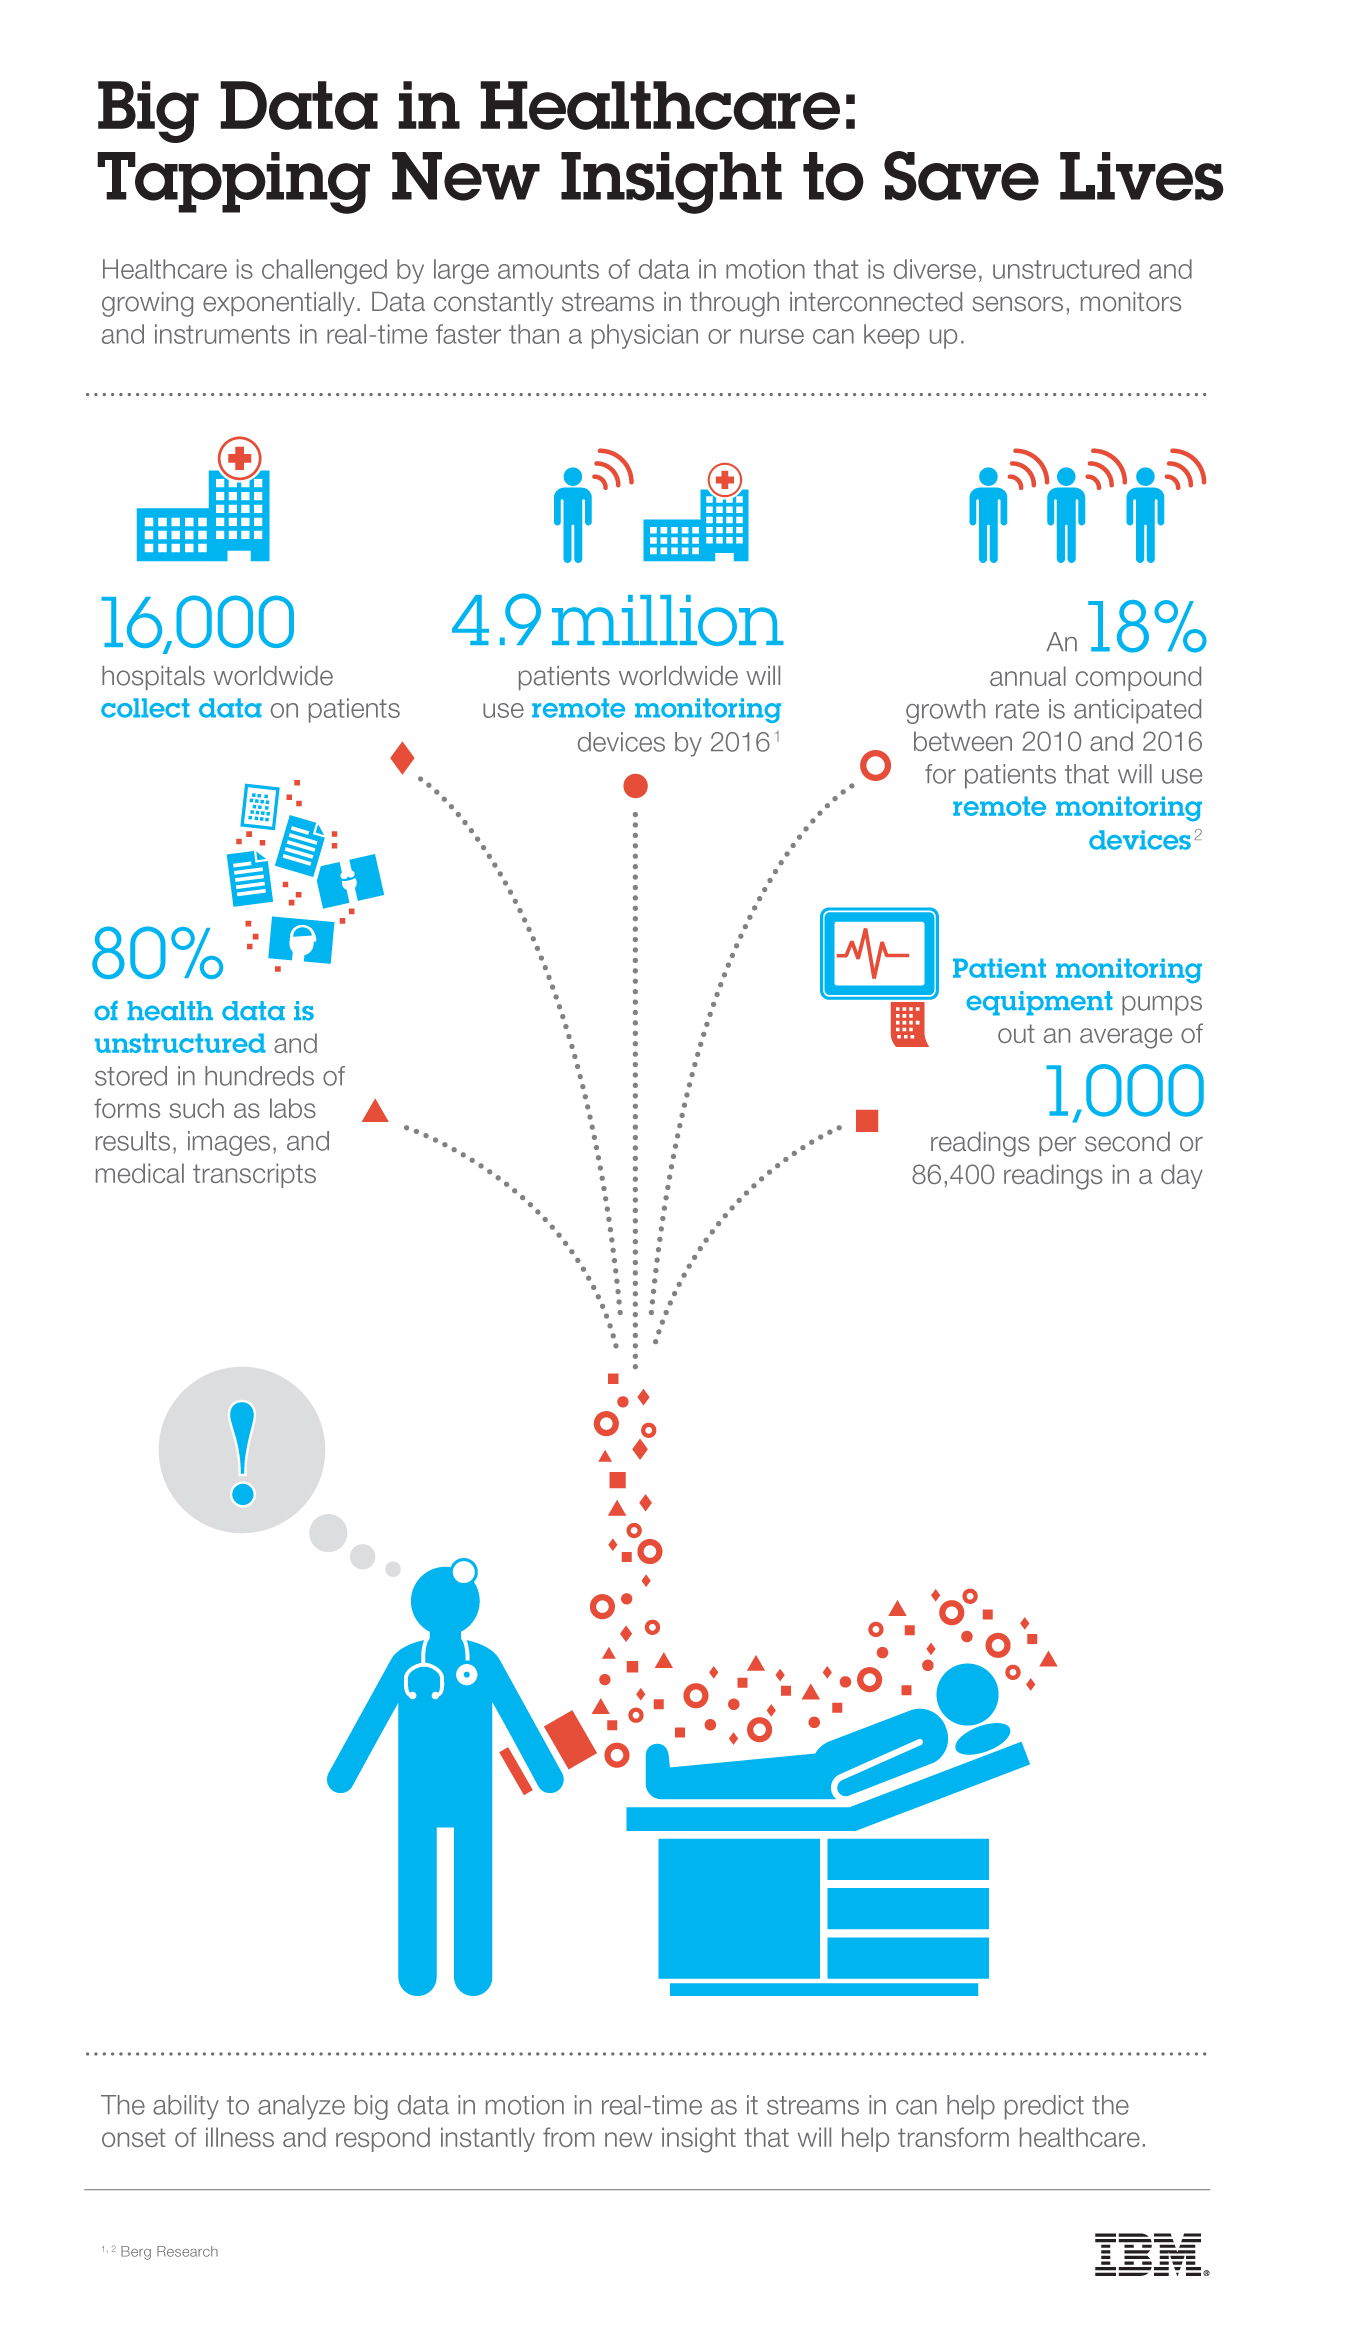
\includegraphics{21.jpg}
\caption{}
\end{figure}

The industry has taken advantage of big data and analytics to make
strategic business decisions. Healthcare big data refers to the
quantities of data that is now available to healthcare providers. The
big data in the healthcare industry is changing the way patients and
doctors handle care. The more big data involved, the more efficient
healthcare can be.

Benefits of Healthcare Big Data:

\begin{itemize}
\tightlist
\item
  Create holistic, 360-degree views of consumers, patients, and
  physicians.
\item
  Improve care personalization and efficiency with comprehensive patient
  profiles.
\item
  Inform physician relationship management efforts by tracking physician
  preferences, referrals, and clinical appointment data.
\item
  Boost healthcare marketing efforts with information about consumer,
  patient, and physician needs and preferences.
\item
  Analyze trends within a single hospital or greater a healthcare
  network to benefit research and care procedures for enhanced
  population health outcomes.
\item
  Identify patterns in health outcomes, patient satisfaction, and
  hospital organization.
\item
  Predict health outcomes and create preventive care strategies with
  data analysis.
\item
  Optimize growth by improving care efficiency, effectiveness, and
  personalization.
\end{itemize}

Below are common questions about Healthcare Big Data:

\begin{itemize}
\tightlist
\item
  What is Driving the Adoption of Big Data in Healthcare?

  \begin{itemize}
  \tightlist
  \item
    Volume of Healthcare Data
  \item
    Government Regulations
  \item
    Desire for Personalized Care
  \end{itemize}
\item
  How Can Marketing Take Advantage of Healthcare Big Data?

  \begin{itemize}
  \tightlist
  \item
    Propensity models (score potential targets)
  \item
    Communication personalization (continue an ongoing relationship with
    the healthcare organization)
  \item
    Integrated communication (holistic customer experiences throughout
    the care continuum)
  \end{itemize}
\item
  What Challenges Arise with Healthcare Big Data?

  \begin{itemize}
  \tightlist
  \item
    Sorting and prioritizing of information
  \item
    Ensuring that the right access to big data insights and analysis
    (data security issues)
  \end{itemize}
\item
  What is the Future of Healthcare Big Data?

  \begin{itemize}
  \tightlist
  \item
    Big data are more crucial for company success
  \item
    Big data healthcare will also smarter and more integrated
  \item
    Big data will grow with Internet of Things (IoT)
  \item
    Iot will become standard methods
  \end{itemize}
\end{itemize}

\subsection{Crime \& Terorism}\label{crime-terorism}

Some police are starting to use big data to predict crime. The use of
fingerprints, DNA, ballistic analysis, CCTV and other types of
technology have also played to improve big data analytics in crime. Top
use case is predictive analytics. This helps in this aspect:

\begin{itemize}
\tightlist
\item
  Police can make compelling cases to get emergency resources to fight
  recent crime waves
\item
  Police can identify the likelihood that they are dealing with serial
  offenders
\item
  Police can look for precipitating factors that cause crime epidemics
  and pass that information along to policymakers to take preventive
  measures
\end{itemize}

Thhe success story of crime prediction are come from RUSI (Royal United
Services Institute for Defence and Security Studies). They published a
paper ``Big Data and Policing An Assessment of Law Enforcement
Requirements, Expectations and Priorities''. One to the success project
is \textbf{Predictive Crime Mapping}

\textbf{How Predictive Crime Mapping Works:}

Big data analytics has been used for a decade for predictive crime
mapping, and the technology continues to be developed and advanced. On
the basic level, this technology is very simple and that are based on:

\begin{itemize}
\tightlist
\item
  Crime type
\item
  Date
\item
  Time
\item
  Crime locations
\end{itemize}

Police officers are printing out their predictive maps to use on patrol
to combat crime in high mapping crime.

**Issues Presented by Using Past Crime \url{Data:**}

These big data solutions are also learning from the past, so the
information can be discriminatory or bias as a result. Example:

100 crimes occurred in the area by males in the past two years. The same
can be inputted for age, religion and race. So, it does present a system
that may create a bias and reinforce this in the police force. If John
Doe is convicted of rape, and all of his rapes occurred on High Street,
algorithms may be able to suggest John Doe as a rapist if:

\begin{itemize}
\tightlist
\item
  Rapes occurred on High Street
\item
  Rapes occurred at around the same time as his previous convictions
\item
  Similar women were raped
\end{itemize}

Of course, it may not be John Doe, but this form of predictive modeling
is an option with big data. It may be possible to scour records, looking
for similar crimes with similar circumstances and tying them together.

\chapter{Big Data Analytics}\label{big-data-analytics}

\section{Data Analytics Lifecycle}\label{data-analytics-lifecycle}

One of the most method for data analytics is \textbf{CRISP-DM
methodology. } The method was found by five companies: SPSS, Teradata,
Daimler AG, NCR Corporation, and OHRA (an insurance company). The
CRISP-DM methodology stands for Cross Industry Standard Process for Data
Mining. It is a robust and well-proven methodology. This model is an
idealised iterative method. Take a look the following illustration.

\begin{figure}
\centering
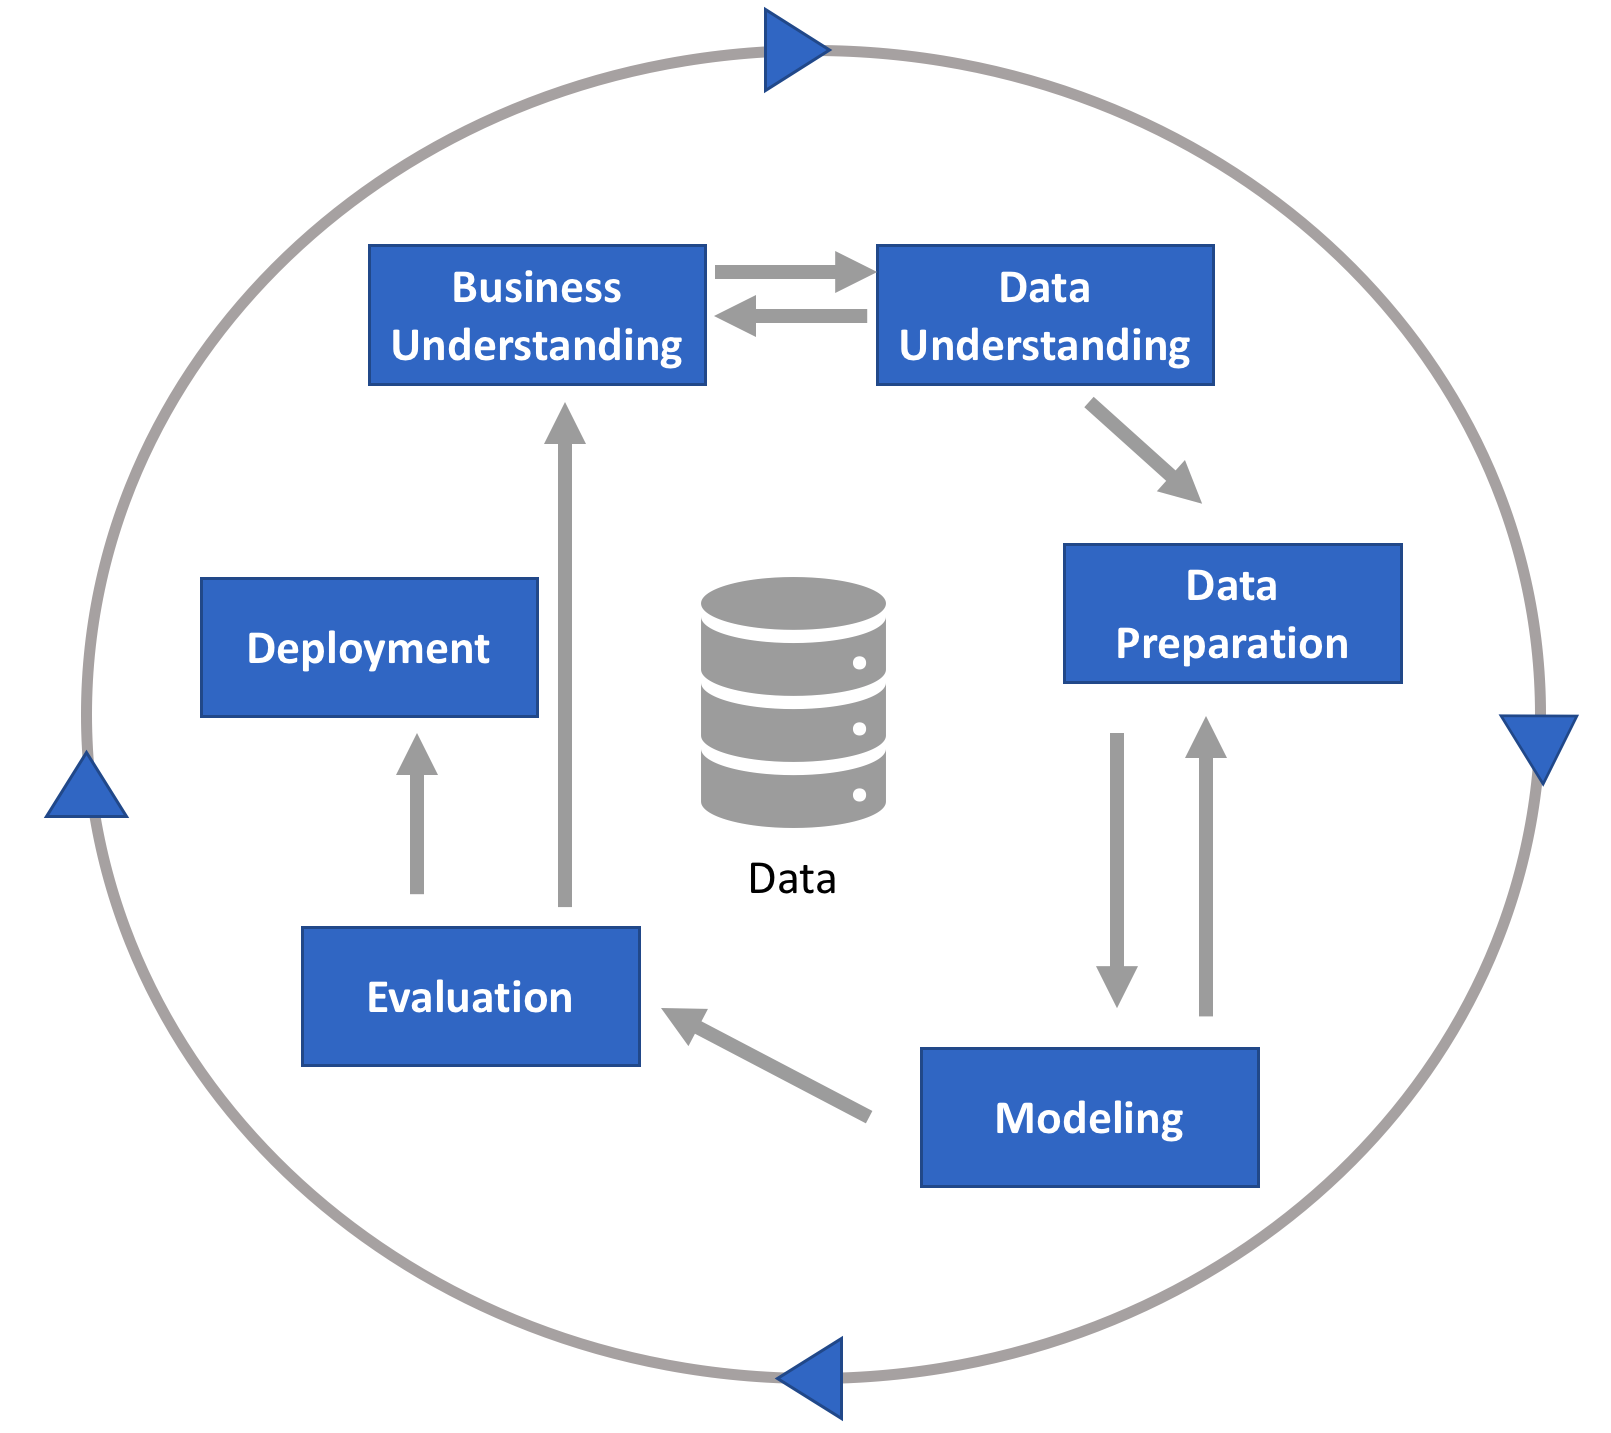
\includegraphics{dm.PNG}
\caption{}
\end{figure}

\textbf{Stage One- Determine Business Objectives }

This initial phase focuses on understanding the project objectives and
requirements from a business perspective. The goal of this stage is to
uncover important factors for improving business. Neglecting this step
can mean that a great deal of effort is put into producing the right
answers to the wrong questions.

What are the desired outputs of the project?

\begin{enumerate}
\def\labelenumi{\arabic{enumi}.}
\item
  \textbf{Set objectives }-It means describing the primary objective
  from a business perspective. For example, your primary goal might be
  to keep current customers by predicting when they are prone to move to
  a competitor. The questions are ``Does the channel used affect whether
  customers stay or go?'' or ``Will lower ATM fees significantly reduce
  the number of high-value customers who leave?''.
\item
  \textbf{Produce project plan }-It describe the plan for achieving
  business needs (improving sales, reduce cost, ect). This step include
  the initial selection of tools and techniques.
\item
  \textbf{Business success criteria }-The successful criteria from the
  business point of view. The criteria should be specific and
  measurable, such as cost reduction or significant sales growth.
\end{enumerate}

Assess the current situation

This involves more details about another factors that company will need
when determining goals.

\begin{enumerate}
\def\labelenumi{\arabic{enumi}.}
\item
  \textbf{Inventory of resources }: The resources available to
  determining business objects including:

  \begin{itemize}
  \tightlist
  \item
    Personnel (business experts, data experts, technical support, data
    mining experts)
  \item
    Data (fixed extracts, access to live, warehoused, or operational
    data)
  \item
    Computing resources (hardware platforms and software)
  \end{itemize}
\item
  \textbf{Requirements, assumptions and constraints }: The list of
  requirements objects that company need. From scheduling, quality
  parameter, data security, and legal issues. Including the assumption
  of the the factors such as verification data and also constraints like
  availability of resources.
\item
  \textbf{Risks and contingencies }: The list of delay project and fail
  probability. what company take if the risk take place?.
\item
  \textbf{Terminology }-A glossary of relevant business and data mining
  terminology.
\item
  Costs and benefits
\end{enumerate}

Determine data analytics goals

Produce the plan

\section{Modern Data Analytics}\label{modern-data-analytics}

\section{Analytics Paradigm}\label{analytics-paradigm}

Analytics helps company answer the business questions. What happened in
the past, what happen in the future, and what decisions company can make
to improving future performance. Nowadays, data analytics is very
important and more and more universities and further education programms
are creating analytics learning environments. \texttt{Tom\ Davenport}
from CIO (Chief Information Officer) Magazine divided analytics area
into three main types of analytics. The three main components of
analytics is as follows:

\begin{figure}
\centering
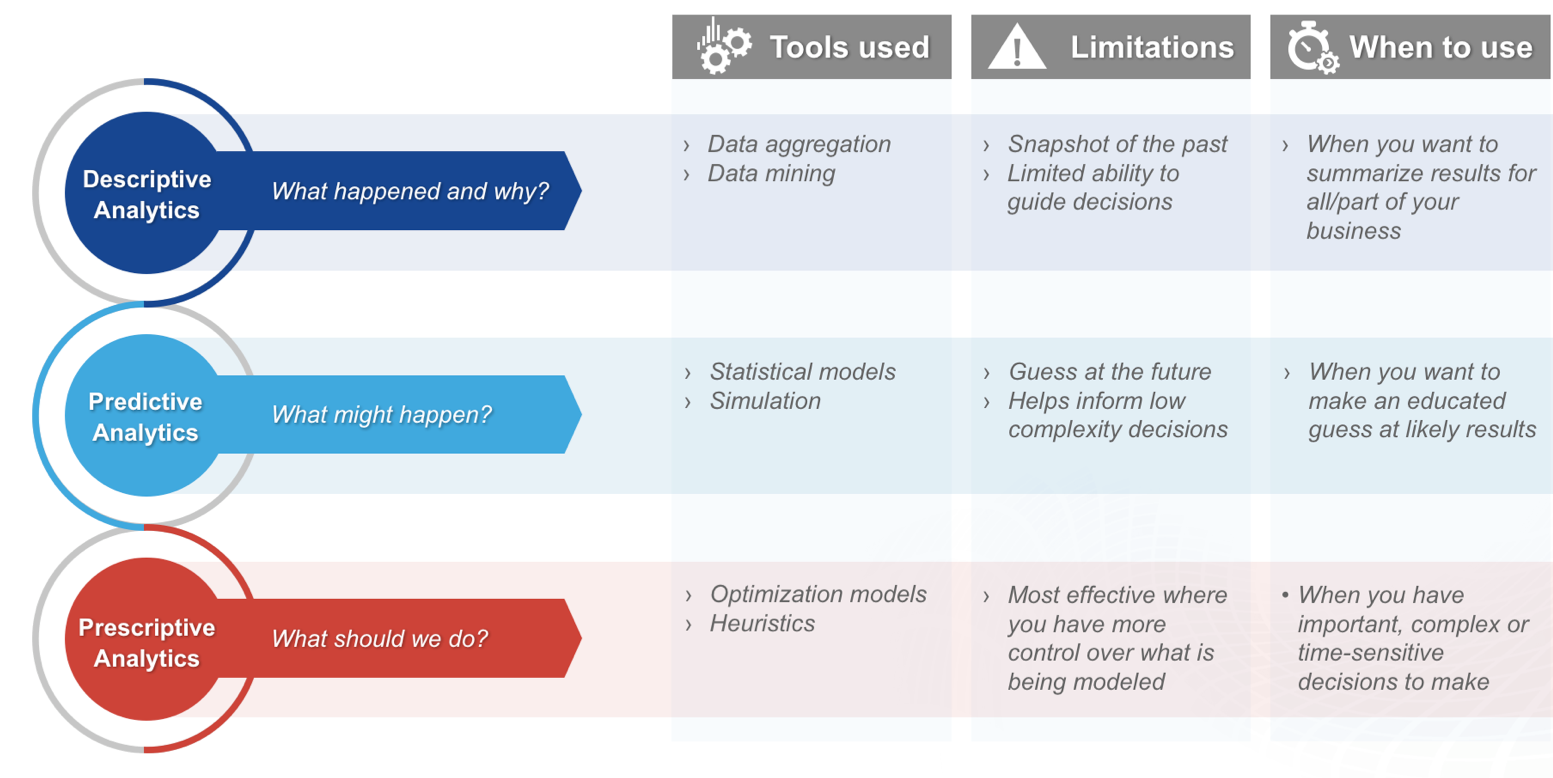
\includegraphics{analytics.png}
\caption{}
\end{figure}

\textbf{Descriptive Analytics: }

Descriptive Analytics helps company to get insight from the past and
current state of business. Most every business function in the company
(Production, Sales, Finance, etc.) used Descriptive Analytics to create
custom reports.

Overview:

\begin{itemize}
\tightlist
\item
  Question being answered: What happened and why?
\item
  Examples of tools used: Data aggregation and data mining
\item
  Limitation to be aware of: Snapshot of the past, often with limited
  ability to help guide decisions
\item
  When to use: When you want to summarize results for all or part of
  your business
\end{itemize}

\textbf{Predictive Analytics: }

Predictive Analytics predicts predicts the business data in the future.
It need applies statistical techniques (often machine learning) to get
what the future may be happen.

Overview:

\begin{itemize}
\tightlist
\item
  Question being answered: What might happen?
\item
  Examples of tools used: Machine learning, statistical models, and
  simulation
\item
  Limitation to be aware of: Guess at the future, helps inform low
  complexity decisions
\item
  When you want to use: When you want to make an educated guess at
  likely results
\end{itemize}

\textbf{Prescriptive Analytics: }

It optimized the set of decisions. Company can quickly evaluate
trillions or more possible combinations of choices (for example: what
products in which manufacturing, what product lines and in what
quantities), minimum production of a given product, manufacturing time
and cost, machine, raw material inventory, finished goods inventory
capacity, and maximize or minimize your objectives (for example: total
product costs).

Overview:

\begin{itemize}
\tightlist
\item
  Question being answered: What should we do?
\item
  Examples of tools used: Optimization and heuristics
\item
  Limitation to be aware of: Most effective where you have some control
  over what is being modeled
\item
  When you want to use: When you have important, interdependent, complex
  or time-sensitive decisions to make
\end{itemize}

\section{Deutsche Bahn Tools}\label{deutsche-bahn-tools}

\subsection{SAP Business Object Web
Intelligence}\label{sap-business-object-web-intelligence}

SAP BO Web Intelligence is databases system created by SAP. The reason
for choosing this databases sytem is \texttt{robust\ software} (from a
few user to tens of thousand of users ) and \texttt{excellent\ service}
from SAP company. This SAP system have some another advantages, such as:

\begin{itemize}
\tightlist
\item
  On-premise deployment (offline)
\item
  Real-time business intelligence (offline and offline)
\item
  Increased user autonomy
\item
  Make information consumption simple, personalized, and dynamic
\end{itemize}

\subsection{Open Refine}\label{open-refine}

Openrefine is a data manipulation tool which cleans, reshapes and
intelligently edit batch messy, and unstructured data. It is an open
source tool and its code can be reused in other projects too. OpenRefine
provides the flexibility to choose from a variety of data set
functionalities, which makes it even more user friendly. Users can use
this tool to get a big view of their data in terms of statistically
curved graphs. They can play with messy data without worrying about
risks.

\textbf{What } --A messy, unstructured, inconsistent dataset can be
explored using open refine. In general, it will be very difficult to
explore data through redundancies and inconsistencies. But, OpenRefine
gives several functions through which one can filter the data, edit the
inconsistencies, and view the data. It's a tool to clean the data.

\textbf{Why }- Spreadsheets can also refine a dataset but they are not
the best tool for it as Openrefine cleans data in a more systematic
controlled manner. While using historical data, we come across issues
like blank fields, duplicate records, inconsistent formats and using
Openrefine tool can help to resolve such issues.

\textbf{When }-Now data analysis play an important role in business.
Data analysts improve decision making, cut costs and identify new
business opportunities. Analysis of data is a process of inspecting,
cleaning, transforming, and modelling data with the goal of discovering
useful information, suggesting conclusions, and supporting decision
making. So, to ensure the accuracy of our analysis, we have to clean our
data.

\textbf{Why OpenRefine is a better tool for data cleaning and modeling:
}

\begin{longtable}[]{@{}lll@{}}
\toprule
\begin{minipage}[b]{0.26\columnwidth}\raggedright\strut
Google refine\strut
\end{minipage} & \begin{minipage}[b]{0.35\columnwidth}\raggedright\strut
Spreadsheets\strut
\end{minipage} & \begin{minipage}[b]{0.30\columnwidth}\raggedright\strut
Databases\strut
\end{minipage}\tabularnewline
\midrule
\endhead
\begin{minipage}[t]{0.26\columnwidth}\raggedright\strut
Batch editing of rows and columns possible\strut
\end{minipage} & \begin{minipage}[t]{0.35\columnwidth}\raggedright\strut
Editing of one cell at a time\strut
\end{minipage} & \begin{minipage}[t]{0.30\columnwidth}\raggedright\strut
Schema and programming language required for editing\strut
\end{minipage}\tabularnewline
\begin{minipage}[t]{0.26\columnwidth}\raggedright\strut
Used for exploring and transforming data\strut
\end{minipage} & \begin{minipage}[t]{0.35\columnwidth}\raggedright\strut
Used for entering data and performing calculations, functions\strut
\end{minipage} & \begin{minipage}[t]{0.30\columnwidth}\raggedright\strut
Data is out of sight unless script is run to view it.\strut
\end{minipage}\tabularnewline
\begin{minipage}[t]{0.26\columnwidth}\raggedright\strut
No Schema Required\strut
\end{minipage} & \begin{minipage}[t]{0.35\columnwidth}\raggedright\strut
No Schema Required\strut
\end{minipage} & \begin{minipage}[t]{0.30\columnwidth}\raggedright\strut
\strut
\end{minipage}\tabularnewline
\begin{minipage}[t]{0.26\columnwidth}\raggedright\strut
Data is always visible at each step of editing\strut
\end{minipage} & \begin{minipage}[t]{0.35\columnwidth}\raggedright\strut
Data is always visible\strut
\end{minipage} & \begin{minipage}[t]{0.30\columnwidth}\raggedright\strut
\strut
\end{minipage}\tabularnewline
\begin{minipage}[t]{0.26\columnwidth}\raggedright\strut
More interactive and visual\strut
\end{minipage} & \begin{minipage}[t]{0.35\columnwidth}\raggedright\strut
Visual is not impressive.\strut
\end{minipage} & \begin{minipage}[t]{0.30\columnwidth}\raggedright\strut
\strut
\end{minipage}\tabularnewline
\bottomrule
\end{longtable}

\subsection{R Programming}\label{r-programming}

R language is an open source program. It maintained by the R core
volunteer developers from across the globe. R is a language and
environment for statistical computing and graphics. It is a GNU project
which is similar to the S language and environment which was developed
at Bell Laboratories (formerly AT\&T, now Lucent Technologies) by
\texttt{John\ Chambers} and colleagues, founded by \texttt{Ross\ Ihaka}
and \texttt{Robert\ Gentlemen}.

\textbf{Key points of R programming:}

\begin{itemize}
\tightlist
\item
  R is open source.
\item
  R programming language is best for statistical, data analysis and
  machine learning.
\item
  R, SAS, and SPSS are three statistical languages. Only R is open
  source
\item
  It supports procedural programming with functions and object-oriented
  programming.
\item
  Packages are part of R programming. Thus, they are useful in
  collecting sets of R functions into a single unit.
\item
  R have database input, exporting data, viewing data, variable labels,
  missing data, etc.
\item
  R is an interpreted language. Hence, we can access it through command
  line interpreter.
\item
  R supports matrix arithmetic.
\item
  It has effective data handling and storage facilities.
\item
  R supports a large pool of operators for performing operations on
  arrays and matrices.
\item
  It has facilities to print the reports for the analysis performed in
  the form of graphs either on-screen or on hardcopy.
\end{itemize}

\textbf{Comparison Of R With Other Technologies:}

\begin{itemize}
\tightlist
\item
  Data handling Capabilities -- Good data handling capabilities and
  options for parallel computation.
\item
  Availability / Cost -- R is an open source and we can use it anywhere.
\item
  Advancement in Tool -- If you are working on latest technologies, R
  gets latest features.
\item
  Ease of Learning -- R has a learning curve. R is a low-level
  programming language. As a result, simple procedures can take long
  codes.
\item
  Job Scenario -- It is a better option for start-ups and companies
  looking for cost efficiency.
\item
  Graphical capabilities -- R is having the most advanced graphical
  capabilities. Hence, it provides you with advanced graphical
  capabilities.
\item
  Customer Service support and community -- R is the biggest online
  growing community.
\end{itemize}

More info about R: \url{https://www.r-project.org/}

\subsection{RStudio}\label{rstudio}

RStudio is a free and open-source integrated development environment
(IDE) for R. RStudio was founded by JJ Allaire,creator of the
programming language ColdFusion. RStudio is available in open source and
commercial editions and runs on the desktop (Windows, macOS, and Linux)
or in a browser connected to RStudio Server or RStudio Server Pro
(Debian, Ubuntu, Red Hat Linux, CentOS, openSUSE and SLES).
(wikipedia.com)

\textbf{RStudio IDE features: }

\begin{itemize}
\tightlist
\item
  An IDE that was built just for R

  \begin{itemize}
  \tightlist
  \item
    Syntax highlighting, code completion, and smart indentation
  \item
    Execute R code directly from the source editor
  \item
    Quickly jump to function definitions
  \end{itemize}
\item
  Bring your workflow together

  \begin{itemize}
  \tightlist
  \item
    Integrated R help and documentation
  \item
    Easily manage multiple working directories using projects
  \item
    Workspace browser and data viewer
  \end{itemize}
\item
  Powerful authoring \& Debugging

  \begin{itemize}
  \tightlist
  \item
    Interactive debugger to diagnose and fix errors quickly
  \item
    Extensive package development tools
  \item
    Authoring with Sweave and R Markdown
  \end{itemize}
\end{itemize}

More info about RStudio: \url{https://www.rstudio.com/}

\subsection{Microsoft Power BI}\label{microsoft-power-bi}

\begin{enumerate}
\def\labelenumi{\arabic{enumi}.}
\tightlist
\item
  What Is Power BI?
\item
  Why Power BI?
\item
  Who Use Power BI?
\item
  Components Of Power BI
\end{enumerate}

\begin{center}\rule{0.5\linewidth}{\linethickness}\end{center}

\begin{enumerate}
\def\labelenumi{\arabic{enumi}.}
\tightlist
\item
  What Is Power BI?
\end{enumerate}

Power BI is a Data Visualization and Business Intelligence tool that
converts data from different data sources to interactive dashboards and
reports. For making best business decisions, it is important to get
relevant information from the data sources and present it as
visualization. Power BI has several products, such as:

\begin{itemize}
\tightlist
\item
  Power BI Desktop: Create rich, interactive reports with visual
  analytics at your fingertips---for free in desktop application.
\item
  Power BI Pro: Connect to hundreds of data sources, and visualize all
  your data with live dashboards and reports. Then share insights across
  your organization to fuel intelligent action.
\item
  Power BI Premium: Power BI Premium offers advanced, self-service data
  preparation that allows every user---from business analyst to data
  scientist---to accelerate the delivery of insights and collaborate
  with ease.
\item
  Power BI Mobile: Stay connected to your data wherever business takes
  you. Mobile business intelligence is just a touch away.
\item
  Power BI Embedded: Embed interactive Power BI visuals in your
  applications, websites, or portals to bring world-class analytics
  directly to your customers
\item
  Power BI Report Server: Power BI Report Server is the on-premises
  solution for reporting today, with the flexibility to move to the
  cloud tomorrow. It's included with Power BI Premium so you have the
  ability to move to the cloud on your terms.
\end{itemize}

For more info: \url{https://powerbi.microsoft.com/en-us/}

\begin{enumerate}
\def\labelenumi{\arabic{enumi}.}
\setcounter{enumi}{1}
\tightlist
\item
  Why Power BI?
\end{enumerate}

\begin{itemize}
\tightlist
\item
  Power BI is built on the convention of best BI products available --
  SQL Server Analysis Services (SSAS) and Microsoft Excel. Power BI
  gives you the option to connect with these products (heavy users
  Microsoft products).
\item
  Power BI is Being built/rebuilt using the latest technologies like
  HTML 5.0, cloud computing, column store databases \& smartphone mobile
  apps.
\item
  Microsoft has opened the custom visuals gallery for open source
  contributions which adds value to the community (from users and
  another company as adds in).

  \begin{itemize}
  \tightlist
  \item
    \url{https://community.powerbi.com/t5/Data-Stories-Gallery/bd-p/DataStoriesGallery}
  \item
    \url{https://appsource.microsoft.com/en-us/marketplace/apps?product=power-bi-visuals}
  \end{itemize}
\item
  Trend towards self-service business intelligence indicates Microsoft's
  leading position in this space. Based on Gartner Research (the world's
  leading research and advisory company) Power BI get high position.
\end{itemize}

\begin{figure}
\centering
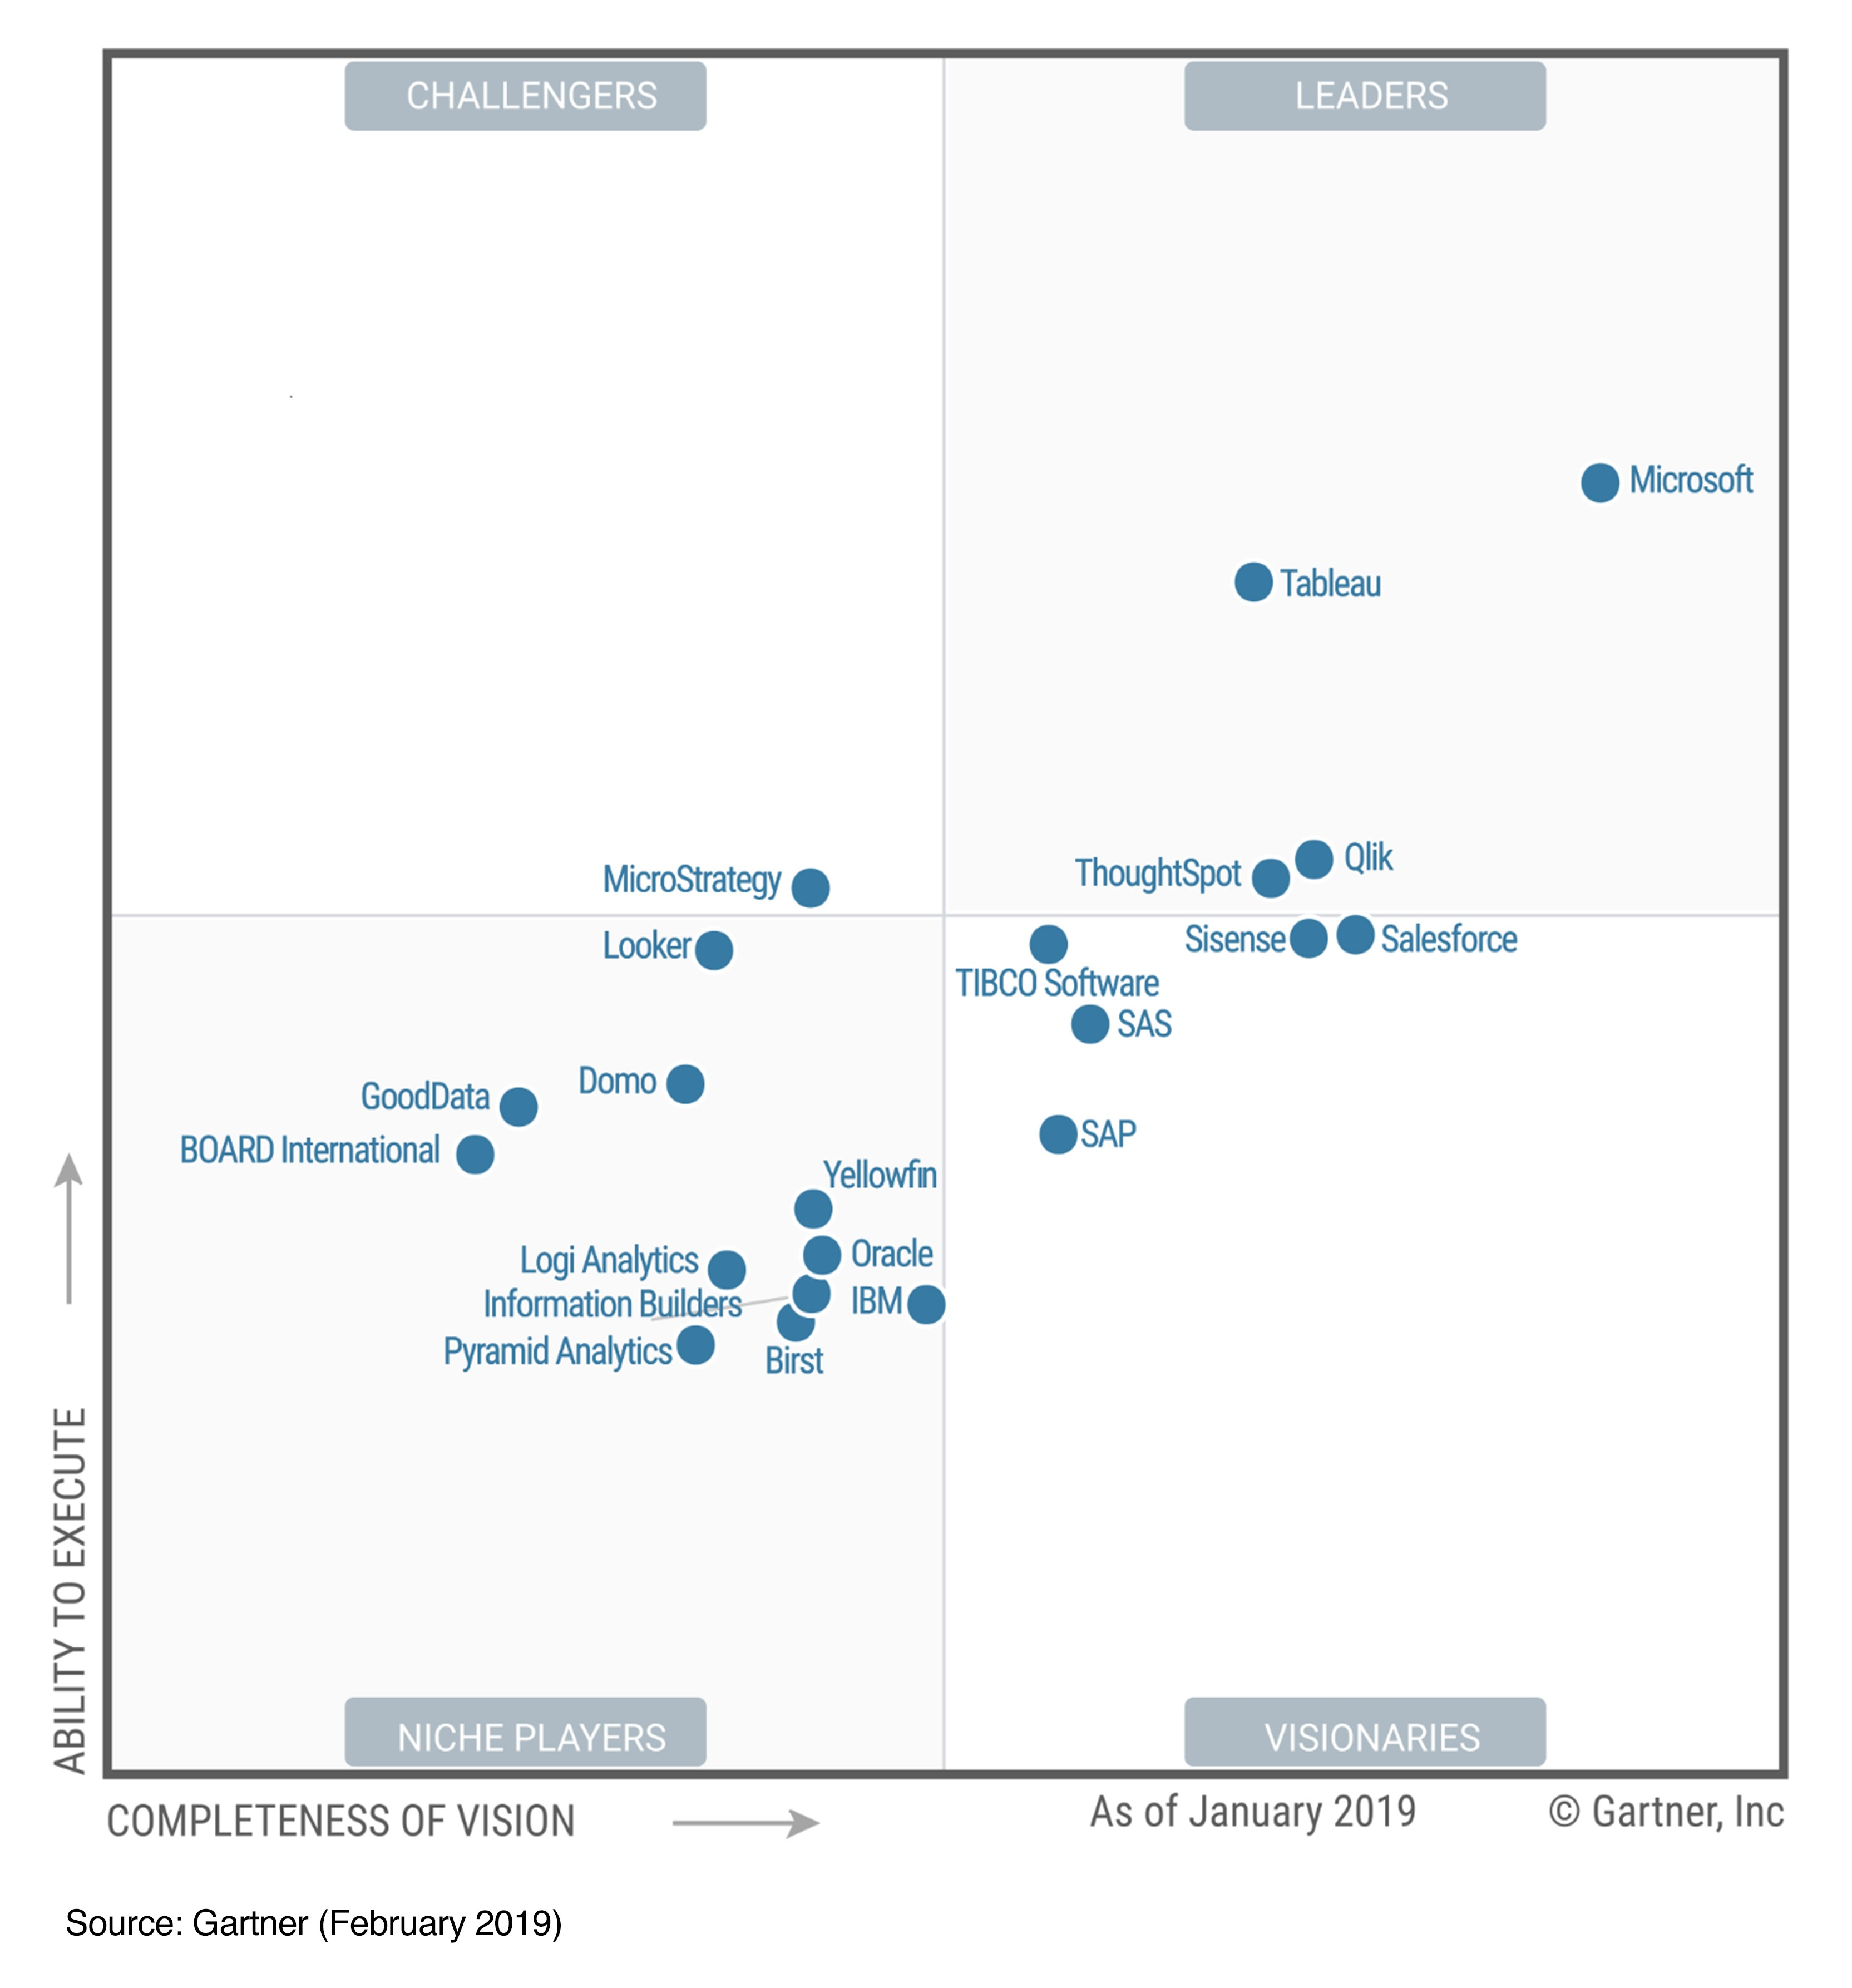
\includegraphics{gartnerpowerbi.jpg}
\caption{}
\end{figure}

\begin{enumerate}
\def\labelenumi{\arabic{enumi}.}
\setcounter{enumi}{2}
\tightlist
\item
  Who Use Power BI?
\end{enumerate}

\begin{itemize}
\tightlist
\item
  Developers
\item
  IT Professional
\item
  Subject Experts (Financial, Insurance, IT Industry, etc)
\item
  Buiness Analyst
\item
  Data Analyst
\item
  Data Scienctist
\item
  Business Intelligence Developer
\end{itemize}

\begin{enumerate}
\def\labelenumi{\arabic{enumi}.}
\setcounter{enumi}{3}
\tightlist
\item
  Components Of Power BI
\end{enumerate}

\begin{itemize}
\tightlist
\item
  Power Query: ETL (Extract, Transform, Loading) data from different
  sources. Power Query Data Sources are:

  \begin{itemize}
  \tightlist
  \item
    Web page
  \item
    Excel or CSV file
  \item
    XML file
  \item
    Text file
  \item
    Folder
  \item
    SQL Server database
  \item
    Microsoft Azure SQL Database
  \item
    Access database
  \item
    Oracle database
  \item
    IBM DB2 database
  \item
    MySQL database
  \item
    PostgreSQL Database
  \item
    Sybase Database
  \item
    Teradata Database
  \item
    SharePoint List
  \item
    OData feed
  \item
    Microsoft Azure Marketplace
  \item
    Hadoop File (HDFS)
  \item
    Microsoft Azure HDInsight
  \item
    Microsoft Azure Table Storage
  \item
    Active Directory
  \item
    Microsoft Exchange
  \item
    Facebook
  \end{itemize}
\end{itemize}

More info about Power Query:
\url{https://docs.microsoft.com/de-de/powerquery-m/power-query-m-reference}

\begin{figure}
\centering
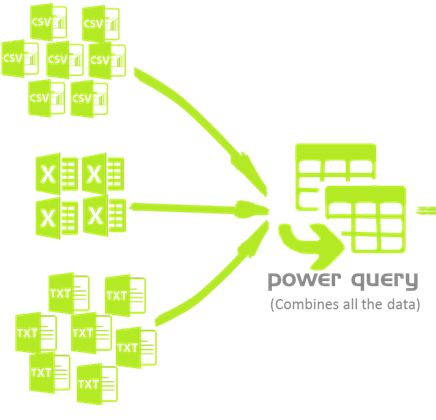
\includegraphics{powerquery.JPG}
\caption{}
\end{figure}

\begin{itemize}
\tightlist
\item
  Power Pivot: Used in data modeling strategy (Snow flakes, Relational,
  Star Schema, etc). Power Pivot have DAX (Data Analysis Expressions) as
  the function programming to help create data model from different
  sources. DAX is a collection of functions, operators, and constants
  that can be used in a formula, or expression, to calculate and return
  one or more values.
\end{itemize}

More info about Power Pivot and DAX:

\begin{itemize}
\tightlist
\item
  \url{https://docs.microsoft.com/en-us/power-bi/desktop-quickstart-learn-dax-basics}
\item
  \url{https://docs.microsoft.com/en-us/dax/dax-function-reference}
\end{itemize}

\begin{figure}
\centering
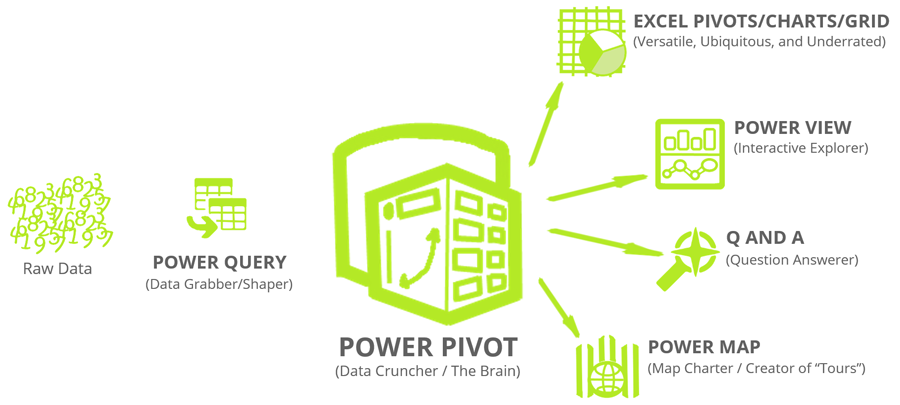
\includegraphics{powerpivot.png}
\caption{}
\end{figure}

\begin{itemize}
\item
  Power View: Analyze, visualize and display data as an interactive data
  visualization.
\item
  Power Map: Interactive geographical visualization.
\item
  Power BI Service: Share data visualization with web browser
  (powerbi.com)
\item
  Power BI Q\&A: Ask questions and get immediate answers with natural
  language query.
\item
  Cortana for Power BI: Cortana is a voice virtual assistant created by
  Microsoft for Power BI.
\end{itemize}

\subsection{Confluence (Software)}\label{confluence-software}

Confluence is a documentation collaboration software program developed
and published by Australian software company Atlassian (atlassian.com).
Confluence is content collaboration tool used to help company to
collaborate and share knowledge efficiently. With Confluence, teams can
create pages and blogs which can be commented on and edited by all
members of the team. It is like microsoft word with additional features.
For mor info: \url{https://www.atlassian.com/software/confluence}

Confluence have about 180 features as documentation cloud software. Here
the complete list:
\url{https://info.seibert-media.net/display/Atlassian/Overview+of+all+180+Confluence+features}

\subsection{Github}\label{github}

Github is open source version control. Version control is a system that
records changes to a file or set of files over time so that you can
recall specific versions later. See the github site:
\url{https://github.com/}

Key Points of Github as Distributed Version Control:

\begin{itemize}
\item
  Keep tracks of changes over time
\item
  Allows the progress and projects to track
\item
  Allows company to revert to earliner versions
\item
  It easier to collaborate with teams
\item
  Track changes on various files (more than one file)
\item
  Track changes on a directory (Track ID)
\item
  Allows savings non-text files (i.e.~images, sheet file, ect)
\item
  Various teams working on the same file
\item
  Use of remote repositories to collaborate
\item
\end{itemize}

DB use Github with RStudio. For more info about how to using Github with
R: \url{https://happygitwithr.com/}

\begin{figure}
\centering
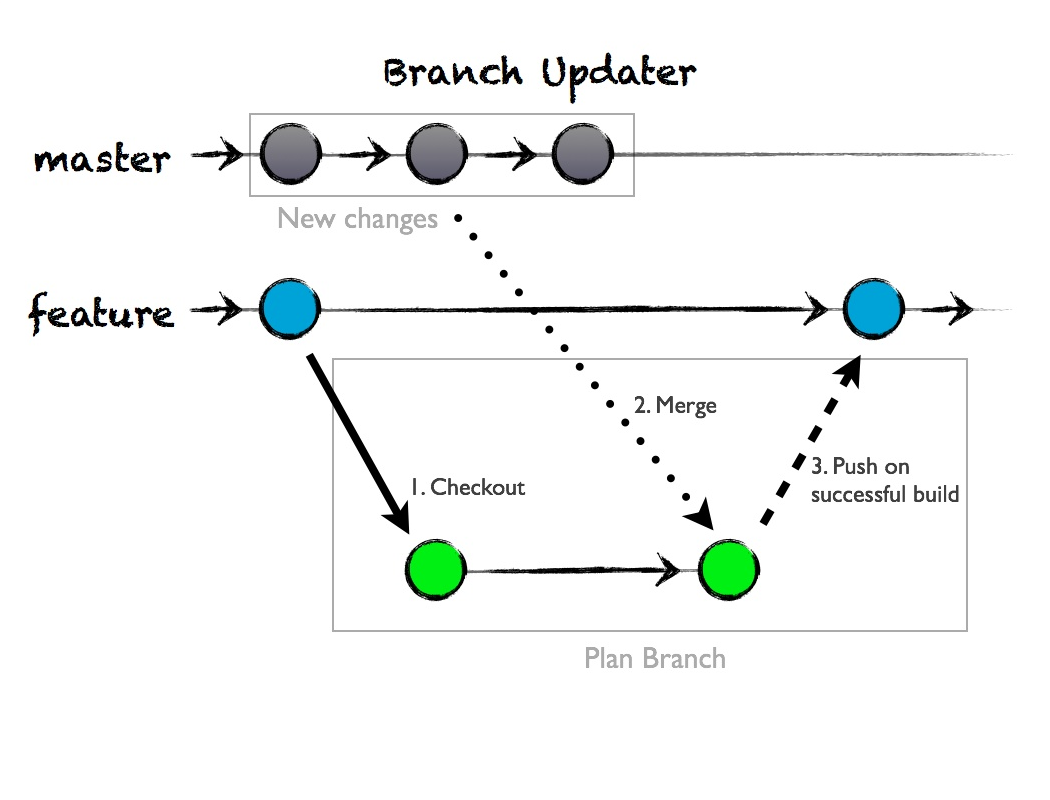
\includegraphics{github1.png}
\caption{}
\end{figure}

\begin{figure}
\centering
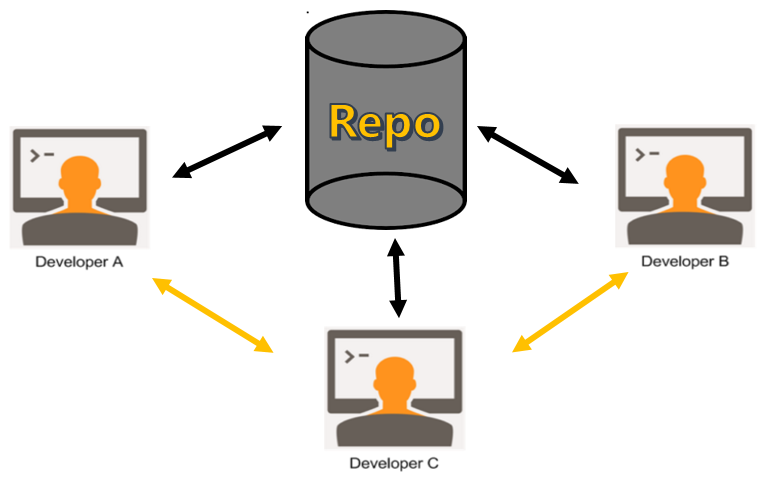
\includegraphics{github2.png}
\caption{}
\end{figure}

\chapter{Terminology}\label{terminology}

\section{Balance Sheet}\label{balance-sheet}

\TeX~is the best way to typeset mathematics. Donald Knuth designed
\TeX~when he got frustrated at how long it was taking the typesetters to
finish his book, which contained a lot of mathematics. One nice feature
of \emph{R Markdown} is its ability to read LaTeX code directly.

If you are doing a thesis that will involve lots of math, you will want
to read the following section which has been commented out. If you're
not going to use math, skip over or delete this next commented section.

\section{Data Cleaning}\label{data-cleaning}

Chemical formulas will look best if they are not italicized. Get around
math mode's automatic italicizing in LaTeX by using the argument
\texttt{\$\textbackslash{}mathrm\{formula\ here\}\$}, with your formula
inside the curly brackets. (Notice the use of the backticks here which
enclose text that acts as code.)

So, \(\mathrm{Fe_2^{2+}Cr_2O_4}\) is written
\texttt{\$\textbackslash{}mathrm\{Fe\_2\^{}\{2+\}Cr\_2O\_4\}\$}.

\noindent Exponent or Superscript: \(\mathrm{O^-}\)

\noindent Subscript: \(\mathrm{CH_4}\)

To stack numbers or letters as in \(\mathrm{Fe_2^{2+}}\), the subscript
is defined first, and then the superscript is defined.

\noindent Bullet: CuCl \(\bullet\) \(\mathrm{7H_{2}O}\)

\noindent Delta: \(\Delta\)

\noindent Reaction Arrows: \(\longrightarrow\) or
\(\xrightarrow{solution}\)

\noindent Resonance Arrows: \(\leftrightarrow\)

\noindent Reversible Reaction Arrows: \(\rightleftharpoons\)

\subsection{Information Technology
Terms}\label{information-technology-terms}

You may wish to put your reaction in an equation environment, which
means that LaTeX will place the reaction where it fits and will number
the equations for you.

\begin{equation}
  \mathrm{C_6H_{12}O_6  + 6O_2} \longrightarrow \mathrm{6CO_2 + 6H_2O}
  \label{eq:reaction}
\end{equation}

We can reference this combustion of glucose reaction via Equation
\eqref{eq:reaction}.

\subsection{Other examples of
reactions}\label{other-examples-of-reactions}

\(\mathrm{NH_4Cl_{(s)}}\) \(\rightleftharpoons\)
\(\mathrm{NH_{3(g)}+HCl_{(g)}}\)

\noindent \(\mathrm{MeCH_2Br + Mg}\) \(\xrightarrow[below]{above}\)
\(\mathrm{MeCH_2\bullet Mg \bullet Br}\)

\section{Data Model}\label{data-model}

Many of the symbols you will need can be found on the math page
\url{http://web.reed.edu/cis/help/latex/math.html} and the Comprehensive
LaTeX Symbol Guide
(\url{http://mirror.utexas.edu/ctan/info/symbols/comprehensive/symbols-letter.pdf}).

\section{Data Analysis Expression
(DAX)}\label{data-analysis-expression-dax}

You will probably find the resources at
\url{http://www.lecb.ncifcrf.gov/~toms/latex.html} helpful, particularly
the links to bsts for various journals. You may also be interested in
TeXShade for nucleotide typesetting
(\url{http://homepages.uni-tuebingen.de/beitz/txe.html}). Be sure to
read the proceeding chapter on graphics and tables.

\chapter{KPIs for big data}\label{kpis-for-big-data}

\textbf{What is KPI? }

KPI (Key Performance Indicators) are the response to company fear of big
data, ugly spreadsheets and uncertain applications with unstructured
data. The idea of KPI is that company presenting big data easily and
also using business relevant language.

Key Performance Indicators are:

\begin{itemize}
\tightlist
\item
  Use rates, ratios, percentages and averages instead of raw numbers
\item
  Leverage tachometers and thermometers and stoplights instead of pie
  charts and bar graphs
\item
  Provide temporal context and highlight change instead of presenting
  tables of data
\item
  Drive business-critical action
\end{itemize}

Measuring the right KPI is vital to the health and success of the
company. Here are 5 reasons why You need KPIs.

\begin{enumerate}
\def\labelenumi{\arabic{enumi}.}
\tightlist
\item
  Monitor company health
\item
  Measuring progress over time
\item
  To make adjustments \& stay on track
\item
  Solving problems and getting more opportunities
\item
  Analyzing patterns over time
\end{enumerate}

Examples of KPIs are:

\begin{itemize}
\tightlist
\item
  Net Profit Margin
\item
  ROI (Return of Investment)
\item
  Operating Cash Flow (OCF)
\item
  Sales Growth
\item
  BEP (Break Event Point)
\item
  Cash Ratio
\end{itemize}

\textbf{Types of KPI }

Depending on your organization's goals and company objectives, they can
track various Key Performance Indicators. The right KPIs right is
crucial for getting actionable and insightful information about the
company's performance and situation.

\begin{quote}
Each business department measures different KPIs because they all have
different tasks and goals.
\end{quote}

There are five main types of KPIs:

\begin{enumerate}
\def\labelenumi{\arabic{enumi}.}
\item
  Business KPI
\item
  Financial KPI
\item
  Sales KPI
\item
  Marketing KPI
\item
  Project Management KPI
\item
  Business KPI
\end{enumerate}

Business KPIs help to measure long-term business goals. By tracking
business KPI, companies are able to understand important business
processes and identify better decision.

Examples of popular business KPIs are:

\begin{itemize}
\tightlist
\item
  Revenue Growth Rate
\item
  Churn Rate
\item
  Acquisition Rate
\item
  Relative Market Share
\item
  Return on Equity
\end{itemize}

\begin{enumerate}
\def\labelenumi{\arabic{enumi}.}
\setcounter{enumi}{1}
\tightlist
\item
  Financial KPI
\end{enumerate}

This KPI provide an assessment of business performance. It is usually
used by an organization's leader and financial department. Financial KPI
indicate how good a company is doing in terms of generating revenue and
profits.

Examples of popular financial KPIs are:

\begin{itemize}
\tightlist
\item
  MRR (Monthly Recurring Revenue)
\item
  Net profit margin
\item
  Operating cash flow (OCF)
\item
  Working Capital
\item
  Current Ratio
\item
  Budget Variance
\end{itemize}

\begin{enumerate}
\def\labelenumi{\arabic{enumi}.}
\setcounter{enumi}{2}
\tightlist
\item
  Sales KPI
\end{enumerate}

Sales KPIs are measurable values that indicates the performance of
various sales processes, used by the sales team to monitor the
achievement of their key objectives and goals. Sales metrics help to
keep and attain sustainable sales.

Example of Popular sales KPI are:

\begin{itemize}
\tightlist
\item
  Monthly New Leads/Sales
\item
  Lead-to-Customer Conversion Rate
\item
  Cost per Acquisition
\item
  Sales Qualified Leads (SQL)
\item
  Customer Lifetime Value (LTV)
\end{itemize}

\begin{enumerate}
\def\labelenumi{\arabic{enumi}.}
\setcounter{enumi}{3}
\tightlist
\item
  Marketing KPI
\end{enumerate}

Marketing KPIs help marketing department to monitor their success across
all marketing channels. A quick overview of marketing metrics shows how
well the marketing team's doing in terms of acquiring new leads.

Examples of popular marketing KPI are:

\begin{itemize}
\tightlist
\item
  Website Traffic Per Source
\item
  Cost Per Acquisition CPA
\item
  Marketing Qualified Leads (MQL)
\item
  Net Promoter Score
\item
  Conversion Rate
\end{itemize}

\begin{enumerate}
\def\labelenumi{\arabic{enumi}.}
\setcounter{enumi}{4}
\tightlist
\item
  Project Management KPI
\end{enumerate}

A project managers used this KPI to monitor project progress. Company
use project KPI to identify successful projects and meet important
deadlines.

Popular Project management KPI are:

\begin{itemize}
\tightlist
\item
  Planned Value (PV)
\item
  Actual Cost (AC)
\item
  Earned Value (EV)
\item
  Cost Variance (CV)
\item
  Schedule Variance (SV)
\end{itemize}

Before we talks about use case in Deutsche Bahn. We need to understand
the types and classification of KPI terms based on perspektive,
industry, and etc.

\textbf{High level vs Low level KPI }

\texttt{High-level\ KPI} demonstrate the company's overall performance.
Examples of high-level KPIs include Annual Growth, Annual Recurring
Revenue (ARR), and Relative Market Share.

Single individuals have no impact on these KPI. They're the result of
teamwork across multiple departments and subsidiary company.

\texttt{Low-level\ KPI} indicate the performance of specific departments
or individuals. Low-level business metrics are tied to people's
day-to-day work and more actionable.

\textbf{Five essential questions for creating a KPI }

\begin{enumerate}
\def\labelenumi{\arabic{enumi}.}
\tightlist
\item
  What are the business results (goals)?
\item
  How can the KPI values be improved by taking action?
\item
  Do we have all the relevant data?
\item
  Who is going to use the KPI?
\item
  How to visualize specific KPI (graphs, metrics, diagrams, etc.)?
\end{enumerate}

\textbf{How to choose the right KPI}

The most important thing is define a business goals. It is better to
focus on a few key metrics instead of many irrelevant ones. Ensure that
every single one of your business metrics meets the SMART criteria:

SMART KPIs are:

\textbf{S }pecific

\textbf{M }easurable

\textbf{A }ttainable

\textbf{R }elevant

\textbf{T }ime-Bound

\textbf{Note }

\begin{itemize}
\tightlist
\item
  \textbf{Understand that Key Performance Indicators } are different for
  each industry, growth stage, and project phase.
\item
  \textbf{A KPI (Key Performance Indicator) } is a measurable value that
  indicates whether a team/company is reaching its targets (benchmarks).
\item
  \textbf{The five main types of KPIs } are business KPIs, financial
  KPIs, sales KPIs, marketing KPIs, and project management KPIs.
\item
  \textbf{KPIs are frequently monitored } with a real-time reporting
  tool -- KPI dashboard.
\item
  \textbf{Each KPI your monitor should meet the SMART criteria },
  i.e.~be Specific, Measurable, Attainable, Relevant, and Time-Bound.
\item
  \textbf{Only track the metrics that are relevant} to your organization
  and business goals.
\end{itemize}

\section{Financial Perspective}\label{financial-perspective}

Based on the size, age, and industry, each and every company needs to be
conscious of their financial situation. The fastest and most efficient
way to keep track of a company business performance is to set up a KPI
that displays financial concern. Let's started with the most widely used
financial metrics that have the full spectrum of important budget.

Firstly, we need to understand the concept of balance sheet. Below is
the example of complete balance sheet.

\begin{figure}
\centering
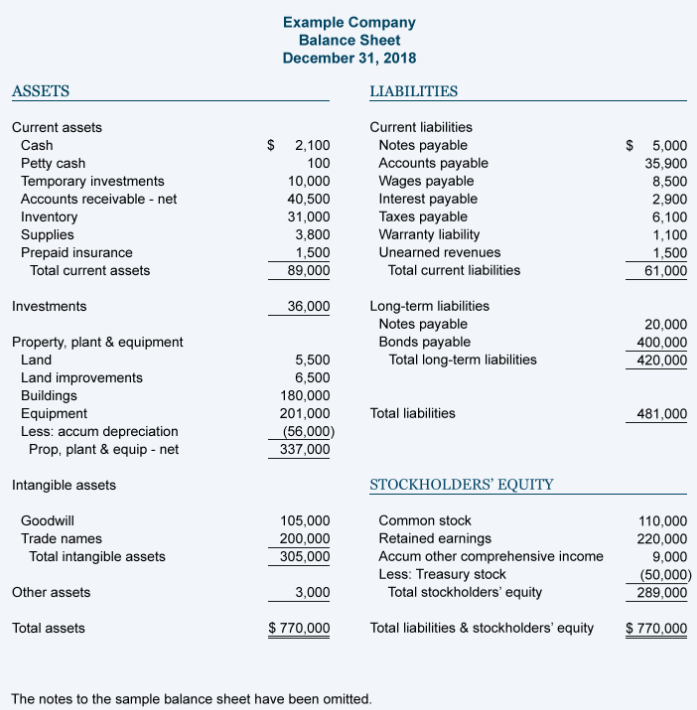
\includegraphics{bs.PNG}
\caption{}
\end{figure}

\subsection{Operating Cash Flow (OCF)}\label{operating-cash-flow-ocf}

How much money generated by the regular operating activities of a
business in a specific time period.

\texttt{Formula\ (short\ form)}: Operating Cash Flow = Net Income +
Non-Cash Expenses -- Increase in Working Capital

\texttt{Formula\ (long\ form)} : Operating Cash Flow = Net Income +
Depreciation + Stock Based Compensation + Deferred Tax + Other Non Cash
Items -- Increase in Accounts Receivable -- Increase in Inventory +
Increase in Accounts Payable + Increase in Accrued Expenses + Increase
in Deferred Revenue

Below is an example of operating cash flow (OCF) using Amazon's 2017
annual report.

\begin{figure}
\centering
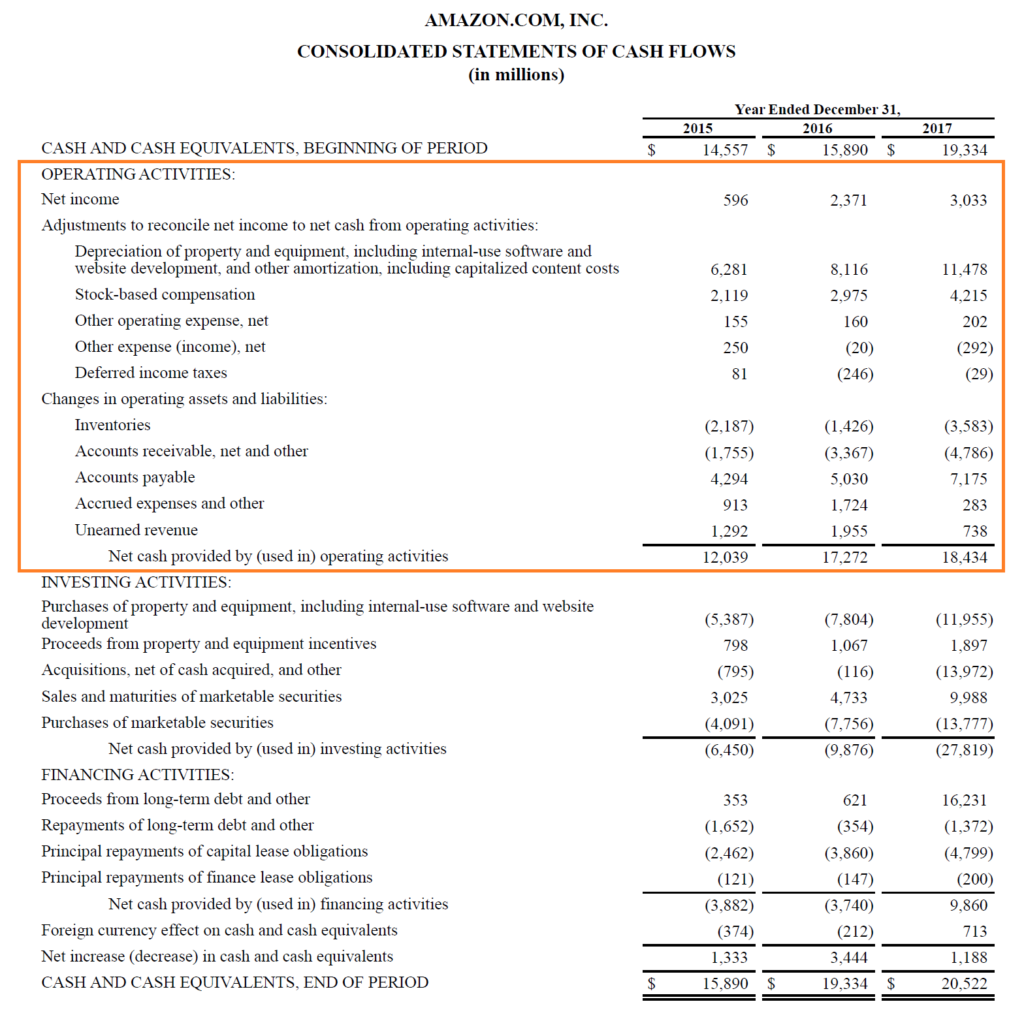
\includegraphics{amazon.png}
\caption{}
\end{figure}

Let's analyze how the operating section counts:

\begin{itemize}
\tightlist
\item
  Net income from the bottom of the income statement is used as the
  starting point
\item
  All non-cash items are ``added back'' meaning any accruals are
  reversed, including:

  \begin{itemize}
  \tightlist
  \item
    Depreciation, which an accounting method for expensing property,
    plant, and equipment (PP\&E) purchases
  \item
    Stock-based compensation is not paid out with actual cash, but
    instead with the issuance of shares
  \item
    Other expense/income could include various items such as unrealized
    gains or losses or accrued items
  \item
    Deferred taxes arise from the difference between accounting methods
    companies use when filing their taxes vs their financial statements
  \end{itemize}
\end{itemize}

\subsection{Current Ratio}\label{current-ratio}

The ability to pay all the financial obligations in one year. A healthy
Current Ratio is between 1.5 and 3

\texttt{Formula}: Current Ratio = Current Assets / Current Liabilities

Example of the Current Ratio Formula:

A business has:

\begin{itemize}
\tightlist
\item
  Cash = \$15 million
\item
  Marketable securities = \$20 million
\item
  Inventory = \$25 million
\item
  Short-term Debt = \$15 million
\item
  Accounts Payables = \$15 million
\end{itemize}

then,

\begin{itemize}
\tightlist
\item
  Current assets = 15 + 20 + 25 = 60 million
\item
  Current liabilities = 15 + 15 = 30 million
\item
  Current ratio = 60 million / 30 million = 2.0x
\end{itemize}

The company can easily settle each accounts payable twice.

\subsection{Ratio / Acid Test}\label{ratio-acid-test}

Indicates whether a business has sufficient short-term assets to cover
its near-future liabilities. The quick ratio deleted liquid assets such
as inventories.

\texttt{A\ common\ alternative\ quick\ ratio\ formula\ is}: (Current
assets -- Inventory) / Current Liabilities

Example:

\begin{longtable}[]{@{}llll@{}}
\toprule
Cash & \$60 & Accounts Payable & \$30\tabularnewline
Marketable Securities & \$10 & Expenses & \$20\tabularnewline
Account Receivables & \$40 & Notes Payable & \$5\tabularnewline
Inventory & \$50 & Long Term Debt & \$10\tabularnewline
Total Current Assets & \$160 & Total Current Liabilities &
\$65\tabularnewline
\bottomrule
\end{longtable}

The Company quick ratio as follows:

(\$60,000 + \$10,000 + \$40,000) / \$65,000 = 1.7

This means that for every money of Company current liabilities, the firm
has \$1.70 of very liquid assets to cover those immediate obligations.

\subsection{Burn Rate}\label{burn-rate}

Burn rate is the amount of time it will take a company to exhaust the
capital. Burn Rate is also in terms of cash burned per month, year , or
quarterly.

\texttt{Formula}: Burn Rate= Cash / Expenses

There are two types of burn rates: net burn and gross burn.

\begin{itemize}
\tightlist
\item
  gross burn: the total amount of operating costs it include in expenses
  each month.
\item
  net burn: the total amount of money a company loses each month.
\end{itemize}

Example:

A company spends \$5,000 monthly on office space, \$10,000 on monthly
server costs and \$15,000 on salaries and wages for its engineers, its
gross burn rate would be \$30,000.

However, if the company was already producing revenue, its net burn
would be different. Even if the company operates at a loss, with
revenues of \$20,000 a month and costs of goods sold (COGS) of \$10,000,
it would still work to reduce its overall burn. In this scenario, the
company's net burn would be \$20,000, derived as: \$20,000 - \$10,000 -
\$30,000 = \$20,000.

\subsection{Net Profit Margin}\label{net-profit-margin}

Indicates how efficient a company at generating profit compared to its
revenue.

\texttt{Formula}: Net profit margin = net profit / revenue

Check this example:

Company ABC and DEF both operate in the same industry. Which company has
a higher net profit margin?

\begin{longtable}[]{@{}llll@{}}
\toprule
Company ABC & Income Statement & Company DEF & Income
Statement\tabularnewline
\midrule
\endhead
Revenue & \$100 & Revenue & \$225\tabularnewline
Cost of Goods Sold & \$20 \_\_- & Cost of Goods Sold & \$35
\_\_-\tabularnewline
Gross Profit & \$80 & Gross Profit & \$195\tabularnewline
Operating Expenses & \$20 \_\_- & Operating Expenses & \$40
\_\_-\tabularnewline
Operating Profit & \$60 & Operating Profit & \$150\tabularnewline
Interest Expense & \$5 \_\_- & Interest Expense & \$10
\_\_-\tabularnewline
Earnings Before Taxes & \$55 & Earnings Before Taxes &
\$140\tabularnewline
Tax Expense & \$25 \_\_- & Tax Expense & \$60 \_\_-\tabularnewline
Net Income & \$30 & Net Income & \$80\tabularnewline
\bottomrule
\end{longtable}

\textbf{Step 1 }: Write out the formula

Net Profit Margin = Net Profit/Revenue

\textbf{Step 2 }: Calculate the net profit margin for each company

Company XYZ:

Net Profit Margin = Net Profit/Revenue = \$30/\$100 = 30\%

Company ABC:

Net Profit Margin = Net Profit/Revenue = \$80/\$225 = 35.56\%

\textbf{Company ABC has a higher net profit margin. }

\subsection{Working Capital}\label{working-capital}

The difference between a current assets (like cash and goods) and
current liabilities (like debts or obligations).

\texttt{Formula}: Working Capital = Current Assets - Current Liabilities

Example:

\begin{longtable}[]{@{}llll@{}}
\toprule
Cash & \$60 & Accounts Payable & \$30\tabularnewline
Marketable Securities & \$10 & Expenses & \$20\tabularnewline
Account Receivables & \$40 & Notes Payable & \$5\tabularnewline
Inventory & \$50 & Long Term Debt & \$10\tabularnewline
Total Current Assets & \$160 & Total Current Liabilities &
\$65\tabularnewline
\bottomrule
\end{longtable}

Using the formula,the working capital ist:

\textbf{\$160 - \$65,000 = \$95 }

\subsection{Current Accounts
Receivable}\label{current-accounts-receivable}

How much money owed by its debtors. This account receivable helps to
estimate the upcoming income.

Let`s take a look the part of balance sheets.

\begin{longtable}[]{@{}llll@{}}
\toprule
Cash & \$60 & Accounts Payable & \$30\tabularnewline
Marketable Securities & \$10 & Expenses & \$20\tabularnewline
\textbf{Account Receivables } & \$40 & Notes Payable &
\$5\tabularnewline
Inventory & \$50 & Long Term Debt & \$10\tabularnewline
Total Current Assets & \$160 & Total Current Liabilities &
\$65\tabularnewline
\bottomrule
\end{longtable}

The account receivable ist \$40.

\subsection{Current Accounts Payable}\label{current-accounts-payable}

How much money owed by its creditors (bank, suppliers, . This account
receivable helps to estimate the upcoming expenses.

Let`s take a look the part of balance sheets.

\begin{longtable}[]{@{}llll@{}}
\toprule
Cash & \$60 & Accounts Payable & \$30\tabularnewline
Marketable Securities & \$10 & Expenses & \$20\tabularnewline
Account Receivables & \$40 & \textbf{Notes Payable } &
\$5\tabularnewline
Inventory & \$50 & Long Term Debt & \$10\tabularnewline
Total Current Assets & \$160 & Total Current Liabilities &
\$65\tabularnewline
\bottomrule
\end{longtable}

The account payable ist \$5.

\subsection{Inventory Turnover}\label{inventory-turnover}

\begin{itemize}
\tightlist
\item
  How efficiently a company sells and replaces its inventory during
  period of time (daily, monthly, or yearly.
\item
  The bility to generate sales and quickly re-stock.
\end{itemize}

\texttt{Formula}: Inventory Turnover = Sales / Inventory or Inventory
Turnover = Cost of Goods Sold / Average Inventory

Example:

Berlin's Paper Company sells office paper. During the current year,
Berlin reported cost of goods sold on its income statement of
\$1,000,000. Berlin's beginning inventory was \$3,000,000 and its ending
inventory was \$4,000,000. Berlin's turnover is calculated like this:

Inventory Turnover= 1,000,000/ {[}(3,000,000+4,000,000)/2)= 0,29

It means that Berlin Paper Company only sold a third (fast 30\%) of its
inventory during the year.

\subsection{Budget Variance}\label{budget-variance}

A budget variance is a different between the predicted cost or revenue
in a given account. (how projected budgets vary compared to actual
budget totals). Optimistic forecasting or poor leadership decisions
caused significant variance (big variance). This KPI used predictive
analytics with mathematical and statistical methoden.

\texttt{Formula}:Predictived Cost - Actual Cost

Not only the cost but also sales, projects budget, ect.

\subsection{Sales Growth}\label{sales-growth}

The growth of sales over a certain period (daily, weekly, quarterly, or
yearly).

\texttt{Formula}: Sales Growth= Current Period Net Sales - Prior Period
Net Sales) / Prior Period Net Sales * 100

Example:

Sales 2018: \$10 Mio Sales 2017: \$5 Mio

So, the sales growth is (10-5)/5*100= 100\%

A Sales hat increased by 100\% than last years.

\subsection{Days Sales Outstanding
(DSO)}\label{days-sales-outstanding-dso}

The average number of days required for clients to pay a company. If the
DSO is lower, company can focus ordering additional supplies.

\texttt{Formula}: DSO= {[}Accounts Receivable / Ne Credit Sales{]} * 365

\begin{itemize}
\tightlist
\item
  Accounts Receivable: \$25,000
\item
  Net Credit Sales: \$200,000
\end{itemize}

So, the DSO is {[}25/200{]} *365= 45.63

It takes 46 days to collect cash from the customers.

\subsection{Payment Error Rate}\label{payment-error-rate}

Uncompleted payments due to a lack of approval, poor documentation or a
missing reference.

\subsection{Complete List}\label{complete-list}

\begin{itemize}
\tightlist
\item
  Profit Indicators

  \begin{itemize}
  \tightlist
  \item
    Earnings before Taxes (EBT)
  \item
    Earnings before Interest and Taxes (EBIT)
  \item
    Earnings before Interest, Taxes and Amortization (ΕΒΙΤΑ)\\
  \item
    Profit or Loss from Ordinary Business Operations
  \item
    Profit or Loss from Extraordinary Operations
  \item
    Operating income from Ordinary Business\\
  \item
    Non-operating income from Ordinary Business
  \item
    Result from Discontinued Operations\\
  \item
    Non-periodic Income\\
  \item
    Net Operating Profit After Taxes (NOPAT)
  \end{itemize}
\item
  Profitability Indicators

  \begin{itemize}
  \tightlist
  \item
    EBIT-Turnover-Yield\\
  \item
    Return On Sales (ROS)\\
  \item
    Return On Equity (ROE)
  \item
    Return On Assets (ROA)
  \item
    Earnings Per Share (EPS)
  \item
    Return On Investment (ROI)
  \item
    Return On Invested Capital (ROIC)
  \item
    Return On Capital Employed (ROCE)
  \item
    Return On Net Assets (RONA)
  \item
    Risk Adjusted Return On Capital (RAROC)
  \item
    Cost-Income Ratio (CIR)
  \end{itemize}
\item
  Liquidity Indicators

  \begin{itemize}
  \tightlist
  \item
    Cash Ratio
  \item
    Quick Ratio
  \item
    Current Ratio
  \item
    Working Capital\\
  \item
    Cash-burn Rate
  \end{itemize}
\item
  Tests of Solvency

  \begin{itemize}
  \tightlist
  \item
    Debt-to-Equity Ratio\\
  \item
    Debt-to-Cash Ratio\\
  \item
    Interest Coverage Ratio
  \end{itemize}
\item
  Cash Flow Measures

  \begin{itemize}
  \tightlist
  \item
    Cash Flow\\
  \item
    Gross or Net Cash Flow\\
  \item
    Free Cash Flow (FCF)\\
  \item
    Operating Cash Flow (OCF)
  \item
    Earnings before Interest, Taxes, Depreciation and Amortization
    (EBITDA)
  \end{itemize}
\item
  Cash Flow Ratios

  \begin{itemize}
  \tightlist
  \item
    Cash Flow Margin\\
  \item
    Cash Flow Return on Investment (CFROI)
  \item
    Cash Flow Return On Equity (CFROE)
  \item
    EBITDA-Turnover-Yield\\
  \item
    Income-Tax Burden Ratio
  \end{itemize}
\item
  Financial Structure Indicators

  \begin{itemize}
  \tightlist
  \item
    Equity-To-Fixed-Assets Ratio (Level I)
  \item
    Equity-To-Fixed-Assets Ratio (Level II)
  \item
    Equity-To-Fixed-Assets Ratio (Level III)
  \item
    Equity Ratio\\
  \item
    Financial Leverage Index
  \end{itemize}
\item
  Efficiency Ratios

  \begin{itemize}
  \tightlist
  \item
    Average Collection Period
  \item
    Average Payment Period\\
  \item
    Cash-to-Cash Cycle\\
  \item
    Asset Turnover Ratio
  \item
    Asset Coverage Period
  \end{itemize}
\item
  Value Based Management (VBM)

  \begin{itemize}
  \tightlist
  \item
    Cash Value Added (CVA)\\
  \item
    Economic Profit (EP)\\
  \item
    Economic Value Added (EVA)\\
  \item
    Weighted Average Cost of Capital (WACC)
  \end{itemize}
\item
  Capital Market Tests

  \begin{itemize}
  \tightlist
  \item
    Market-to-Book Ratio\\
  \item
    Stock Yield\\
  \item
    Dividend Yield
  \item
    Price-Earnings Ratio (P/E Ratio)
  \item
    Price-To-Cash Flow Ratio
  \item
    Cash Flow per Share
  \end{itemize}
\item
  Capital Budgeting Tests

  \begin{itemize}
  \tightlist
  \item
    Payback Period
  \item
    Time Adjusted or Discounted Payback Period
  \end{itemize}
\end{itemize}

\section{Customer Perspective}\label{customer-perspective}

According to research from walkerinfo.com (customer research
consulting), customer satisfication will overtake as the key success.
Company require volumes of customers, number contacts, and number
employees, and another data as a key factors. It depend on the situation
and company business model.

Below are example of the most using KPI for Customer Perspektive:

\subsection{Customer Satisfaction Score
(CSAT)}\label{customer-satisfaction-score-csat}

Measuring CSAT is very hard. Customers need to express an emotion, and
emotions are harder to indentify than objective facts. CSAT can consist
of regular numbers, some icon (like stars, smiley faces, etc).

Example: Users uses a 5 stars scale for ratings

\begin{figure}
\centering
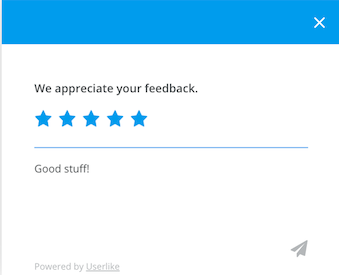
\includegraphics{csat.PNG}
\caption{}
\end{figure}

\subsection{Net Promoter Score (NPS)}\label{net-promoter-score-nps}

How likely customers are referring the products to someone else.

Example: Company ask the customers how likely they are to recommend the
products on a scale from 1 to 10.

\begin{figure}
\centering
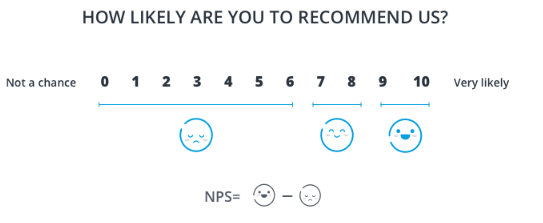
\includegraphics{nps.PNG}
\caption{}
\end{figure}

\subsection{First Response Time}\label{first-response-time}

Customers are changed like the Spice Girls: ``If you wanna get with me,
better make it fast!''. The Customers expect an excellent shopping
experience. A Salesforce study found that a third of the respondents
felt positive about companies that offered a quick first response. First
Response Time is calculated by subtracting the time of the request from
the time of the initial reply.

\begin{figure}
\centering
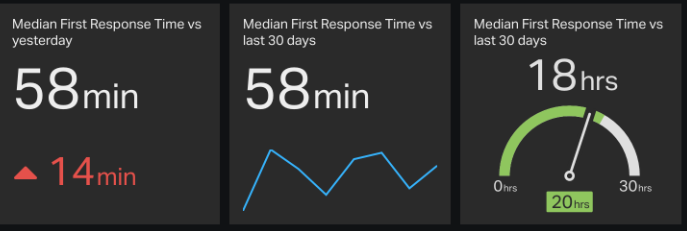
\includegraphics{ftr.PNG}
\caption{}
\end{figure}

\subsection{Customer Retention Rate}\label{customer-retention-rate}

The ability to keep a customer over a set period of time (daily,
monthly, yearly).

\texttt{Formula}: Customer Retention Rate = ((CE -- CN) / CS)) x 100

\begin{itemize}
\tightlist
\item
  CE = Number of customers at end of period
\item
  CN = Number of new customers acquired during period
\item
  CS = Number of customers at start of period
\end{itemize}

\subsection{Employee Engagement}\label{employee-engagement}

The KPI about employees satisfication. The standars approach ist direct
ask. Another method is survei. The survey should consist of the
following engagement levels:

\begin{itemize}
\tightlist
\item
  Management quality and time investment
\item
  Influence from colleagues
\item
  Relationships
\item
  Work schedule
\end{itemize}

Another example of customer perspektive are:

\begin{itemize}
\tightlist
\item
  Annual sales/customers(\$)
\item
  Average custome size(\$)
\item
  Customer rating(\%)
\item
  Average time from customer contact to sales response(No)
\item
  Average time spent on customer relations(No)
\item
  Customers/employee ( No or \%)
\item
  Satisfied-customer index(\%)
\item
  Customer-loyalty index(\%)
\item
  Market Share
\item
  No of Customer Complaints
\item
  Return Rates
\item
  Response Time
\item
  Cost/customer(\$)
\item
  Customers Lost(No or \%)
\item
  Customer retention
\item
  Number of customers
\item
  Annual sales per customer
\item
  Marketing cost as a \% of sales(\%)
\item
  Marketing expenses(\$)
\item
  Number of proposals made
\item
  Brand-image index (\%)
\item
  Response rate
\item
  Sales volume
\item
  Sales per channel
\item
  Average customer size
\item
  Customers per employee
\item
  Frequency of sales transactions
\item
  Sales closed/sales contacts(\%)
\item
  Number of visits to customers(No)
\item
  Service expense/customer/year(\$)
\end{itemize}

\subsection{Complete List}\label{complete-list-1}

\begin{itemize}
\tightlist
\item
  Customer Relationship Management (CRM)

  \begin{itemize}
  \tightlist
  \item
    Customer Acquisition Rate 133 3.1.2
  \item
    Customer Churn Rate 134 3.1.3
  \item
    Customer Retention Period 136 3.1.4
  \item
    Customer Significance Level 138 3.1.5
  \item
    Cross-Selling Ratio 140 3.1.6
  \item
    Customer Lifetime Value (CLV) 141 3.1.7
  \item
    Customer Satisfaction Index 143 3.1.8
  \item
    Customer Complaint Ratio 146 3.1.9
  \item
    Flop Rate
  \end{itemize}
\item
  Marketing Communication Indicators

  \begin{itemize}
  \tightlist
  \item
    Media Coverage Level 150 3.2.2
  \item
    Click Through Rate (CTR) 152 3.2.3
  \item
    Conversion Rate 153 3.2.4
  \item
    Cost per Thousand 155 3.2.5
  \item
    Brand Awareness Level
  \end{itemize}
\item
  Product Pricing

  \begin{itemize}
  \tightlist
  \item
    Profit Margin
  \item
    Gross Margin
  \item
    Absolute Contribution Margin\\
  \item
    Percentage Contribution Margin\\
  \item
    Price Reduction Rate\\
  \item
    Direct Product Profit (DPP)\\
  \item
    Price Elasticity of Demand (PEoD)\\
  \item
    Purchasing Power Index
  \end{itemize}
\item
  Cost-Profit-Volume Analysis

  \begin{itemize}
  \tightlist
  \item
    Break-Even Point (BEP)\\
  \item
    Margin of Safety\\
  \item
    Margin of Safety-Factor\\
  \item
    Cash Point
  \end{itemize}
\item
  Market Coverage Indicators

  \begin{itemize}
  \tightlist
  \item
    Internationalization Level\\
  \item
    Distribution Coverage Level
  \item
    Customer Coverage Ratio\\
  \item
    Market Saturation Level
  \end{itemize}
\item
  Market Position Indicators

  \begin{itemize}
  \tightlist
  \item
    Absolute Market Share\\
  \item
    Relative Market Share
  \item
    Bid Acceptance Rate
  \end{itemize}
\item
  Sales Efficiency Indicators

  \begin{itemize}
  \tightlist
  \item
    Sales per Reference Parameter\\
  \item
    Contribution Margin per Reference Parameter\\
  \item
    Sales Space Productivity\\
  \item
    Capacity Coverage Ratio\\
  \item
    Book-to-Bill Ratio\\
  \item
    Finished Goods Turnover Period
  \end{itemize}
\end{itemize}

\section{Process Perspective}\label{process-perspective}

\subsection{Cost performance index
(CPI)}\label{cost-performance-index-cpi}

The financial effectiveness and efficiency of a project. For example, if
a project has a earned value of £30,000 but actual costs were £12,000.

\begin{quote}
CPI = EV / AC = 30,000 / 12,000 = 2.5
\end{quote}

If the ratio has a value higher than 1 then it indicates the project is
performing good.

\subsection{Schedule Performance Index
(SPI)}\label{schedule-performance-index-spi}

Indicates how efficiently the company actually progressing compared to
the planned project schedule. It is the efficiency of the time on the
project.

\texttt{Formula}: Schedule Performance Index = (Earned Value) / (Planned
Value)

Example:

A Company have a project to becompleted in 12 months, and the budget of
the project is 100,000 USD. Six months have passed, and 60,000 USD has
been spent, but on closer review, you find that only 40\% of the work
has been completed so far.

\begin{longtable}[]{@{}l@{}}
\toprule
Given in the question:\tabularnewline
\midrule
\endhead
Actual Cost (AC) = \$60,000\tabularnewline
Planned Value (PV) = 50\% of \$100,000\tabularnewline
= \$50,000\tabularnewline
Earned Value (EV) = 40\% of \$100,000\tabularnewline
= \$40,000\tabularnewline
And then,\tabularnewline
Schedule Performance Index (SPI) = EV / PV\tabularnewline
= 40,000 / 50,000\tabularnewline
= 0.8\tabularnewline
\bottomrule
\end{longtable}

The Schedule Performance Index is 0.8

This Company is behind schedule since the Schedule Performance Index is
less than one.

\subsection{Complete List}\label{complete-list-2}

\begin{itemize}
\tightlist
\item
  Project Controlling

  \begin{itemize}
  \tightlist
  \item
    Schedule Performance Index (SPI)\\
  \item
    Cost Performance Index (CPI)
  \item
    Time Estimation at Completion (TEAC)
  \item
    Estimate at Completion (EAC)
  \item
    To-Complete-Performance Index (TCPI)\\
  \item
    Process Acceleration Costs
  \end{itemize}
\item
  Quality Controlling

  \begin{itemize}
  \tightlist
  \item
    Quality Rate
  \item
    Rejection Rate
  \item
    Follow-up Costs Ratio\\
  \item
    Conformity Costs Ratio\\
  \item
    Non-Conformity Costs Ratio
  \end{itemize}
\item
  Supply Chain Management

  \begin{itemize}
  \tightlist
  \item
    Procurement Efficiency Ratio\\
  \item
    Supply Chain Cycle Time\\
  \item
    Faulty Incoming Delivery Rate\\
  \item
    Faulty Outgoing Delivery Rate
  \item
    Vertical Integration Level\\
  \item
    Supplier's Service Level
  \item
    Cooperation Index
  \end{itemize}
\item
  Production Capacity Management

  \begin{itemize}
  \tightlist
  \item
    Plant Availability Time\\
  \item
    Plant Downtime Rate 236
  \item
    Maintenance Cost Intensity\\
  \item
    Capacity Utilization Level\\
  \item
    Contribution Margin per Unit of the Constrained Resource
  \end{itemize}
\item
  Process Controlling

  \begin{itemize}
  \tightlist
  \item
    Throughput Time (TPT)
  \item
    Days Inventory Outstanding (DIO)\\
  \item
    Inventory Turnover Ratio\\
  \item
    Material Coverage Period\\
  \item
    Process Cost Rate
  \item
    Expected Process-based Loss
  \item
    Machine Hour Rate\\
  \item
    Bottleneck-induced Incremental Costs
  \end{itemize}
\item
  Sustainability Management

  \begin{itemize}
  \tightlist
  \item
    Resource Consumption Level\\
  \item
    Resource Consumption Efficiency Level\\
  \item
    Sustainable Value
  \item
    Emission Volume of Production-related Pollutants
  \item
    Emission Volume of Usage-related Pollutants\\
  \item
    Disposal Costs Ratio\\
  \item
    Recycling Ratio
  \end{itemize}
\end{itemize}

\section{Human Resource and Innovation
Perspective}\label{human-resource-and-innovation-perspective}

\textbf{Retention }

The basic formula for employee retention is the following:

\begin{quote}
(\# of employees who stayed at the company for the whole time
period)/(\# employees at start of the time period) X 100
\end{quote}

Example : If 90 people were working at my company as of June 1st and 80
of those same people were still working at my company as of June 30th,
my retention rate for the month of June would be the following: 80/90 *
100 = 88.9\%

\textbf{Time in The Position } How long are employees in the same
position

\textbf{Absenteeism }

\begin{itemize}
\tightlist
\item
  Delays
\item
  Sick leave
\item
  Excused or unexcused absenses
\end{itemize}

\textbf{Recruitment Time }

Time between employee leaving and another candidate selected to replace
him.

\textbf{Education }

The courses for employee that has direct impact on the company
performances.

\textbf{Time to Achieve Goals }

The efficiency of the workforce to see how long it takes to finish the
tasks.

\textbf{Accidents at Work }

The number of accidents in the workplace.

\textbf{Complete List: }

\begin{itemize}
\tightlist
\item
  Personnel Cost Management

  \begin{itemize}
  \tightlist
  \item
    Personnel Costs Ratio 283 5.1.2
  \item
    Supplementary Personnel Costs Ratio 285 5.1.3
  \item
    Personnel Costs per Employee 287 5.1.4
  \item
    Unit Labor Cost
  \end{itemize}
\item
  Human Resource Controlling

  \begin{itemize}
  \tightlist
  \item
    Labor Productivity
  \item
    Overtime Quota\\
  \item
    Workforce Composition Ratios\\
  \item
    Internally-staffed Executive Positions Ratio
  \item
    Staff Recruitment Period
  \end{itemize}
\item
  Human Resource Development Indicators

  \begin{itemize}
  \tightlist
  \item
    Apprenticeship Quota
  \item
    Trainee Absorption Rate
  \item
    Professional Development Training Time per Employee\\
  \item
    Professional Development Training Costs Ratio
  \end{itemize}
\item
  Organizational Behavior Indicators

  \begin{itemize}
  \tightlist
  \item
    Labor Turnover Rate\\
  \item
    Employees Satisfaction Index\\
  \item
    Sickness-Absenteeism Rate
  \item
    Accident Occurrence Rate\\
  \item
    Participation Rate in Ideas Management
  \end{itemize}
\item
  Innovativeness

  \begin{itemize}
  \tightlist
  \item
    Innovation Rate\\
  \item
    Research and Development Intensity (R\&D Intensity)
  \item
    Research and Development Costs Ratio (R\&D Costs Ratio)\\
  \item
    Break-Even Time
  \end{itemize}
\end{itemize}

\section{By Industry}\label{by-industry}

\subsection{T \& L Industry}\label{t-l-industry}

Example KPIs for the Transportation and Logistic (Warehousing) Industry:

\begin{itemize}
\tightlist
\item
  Annualized inventory turns: a ratio showing how many times a company
  has sold and replaced inventory during a given period (years, months,
  10 years).
\item
  Annualized cost of goods sold (COGS)/average daily inventory value
\item
  Backlog value
\item
  Value of open, not yet fulfilled, booked order lines
\item
  Book to fulfill ratio
\item
  Booked order value/fulfilled value
\item
  Book to ship days
\item
  Average of shipped date - Firm date (booked date used if no firmed
  date)
\item
  Booked order value
\item
  Booked order line value (not including returns)
\item
  Claims percentage for freight costs
\item
  Customer order promised cycle time
\item
  Defects per million opportunities
\item
  Inventory months of supply
\item
  On-time line count
\item
  On-time pickups
\item
  Pick exceptions rate
\item
  Percentage of picks with exceptions
\item
  Pick release to ship
\item
  Planned inventory turns
\item
  Planned cost of goods sold/planned inventory value
\item
  Planned margin
\item
  Planned revenue - Planned costs
\item
  Planned margin percentage
\item
  Planned margin/planned revenue
\item
  Planned on-time shipment
\item
  Planned service level (percentage of shipments shipped on time)
\item
  Planned resource utilization
\item
  Planned resource usage
\item
  Product revenue
\item
  Product sales revenue (not including service) recognized in selected
  period (based on AR invoice lines)
\item
  Product revenue backlog
\item
  Value of booked order lines less returns plus deferred revenue backlog
  (invoiced but not recognized) Production value
\item
  Value of work-in-process (WIP) completions into inventory
\item
  Production to plan rate
\item
  Production standard value/planned standard value
\item
  Receipt to put-away
\item
  Time elapsed from pick release to ship confirm
\item
  Time elapsed from receipt
\item
  Transit time
\end{itemize}

\subsection{Wholesale Trade}\label{wholesale-trade}

Example KPIs for the Wholesale Trade Industry:

\begin{itemize}
\tightlist
\item
  Dock turnaround time
\item
  Freight costs (minimize costs without affecting deliveries)
\item
  Inventory accuracy, stockouts
\item
  Inventory carrying costs
\item
  Inventory turns per year
\item
  Logistics costs per year
\item
  Low-velocity inventory comparison through sectors
\item
  Order fill rate and accuracy
\item
  Technology used to execute inventory strategies
\item
  Warehouse flow-through (or some measure of yard or warehouse
  productivity)
\item
  Wholesale revenue
\item
  Total factor productivity
\item
  Labor productivity
\item
  Return on assets
\item
  Profit margin
\item
  Debt to equity
\item
  Inventory turnover
\item
  Asset utilization
\item
  Collection efficiency
\end{itemize}

\subsection{Utilities Industry}\label{utilities-industry}

Example KPIs for the Utilities Industry:

\begin{itemize}
\tightlist
\item
  Annual labor cost per device
\item
  Average cost per job category
\item
  Average cost per megawatt produced
\item
  Average labor hours per device per year
\item
  Average maintenance cost per mile of pipe/line/cable
\item
  Average number of days each work order is past due
\item
  Average number of labor hours to complete a maintenance task
\item
  Average response time to fix breaks
\item
  Average revenue per megawatt produced
\item
  Average time to settle a rate case
\item
  Consumption analyzed by units consumed and target reduction achieved
\item
  Crew productivity
\item
  Drinking water quality - Percentage of water tests that meet
  regulatory standards
\item
  Electrical grid load
\item
  Equipment failure rate
\item
  Equipment unavailability, hours per year - Planned maintenance
\item
  Equipment unavailability, hours per year - Sustained fault
\item
  Equipment unavailability, hours per year - Temporary fault
\item
  Equipment unavailability, hours per year - Unplanned maintenance
\item
  Maintenance backlog
\item
  Maintenance cost as a percentage of manufacturing cost
\item
  Maintenance technician's skill level improvement, year over-year
\item
  Mean time to repair
\item
  Number of complaints received by type
\item
  Number of customers who were cut off due to violations of regulations
\item
  Number of disconnections
\item
  Number of pending work orders
\item
  Number of power failures per year
\item
  Number of reported gas leakages per 1,000 households
\item
  Number of sewage blockages per month/year
\item
  Number of staff per 1,000 customer connections
\item
  Number of uncontrolled sewage overflows affecting private properties
\item
  Outage time per event
\item
  Percentage of customers that would characterize their bills as
  accurate and timely
\item
  Percentage of possible power revenue billed
\item
  Percentage reduction in number of complaints to the local regulatory
  body
\item
  Percentage reduction in number of employee injuries
\item
  Percentage reduction in number of equipment failures
\item
  Percentage of maintenance work orders requiring rework
\item
  Percentage of man-hours used for proactive work
\item
  Percentage of scheduled man-hours to total man-hours
\item
  Profit redistribution (rural electric coops)
\item
  Reduction in hazardous liquid spill notification time
\item
  Reduction or stabilization in rates (municipally owned utilities)
\item
  Response time to gas or water leaks
\item
  Sewage system reliability
\item
  Station unavailability - Planned maintenance
\item
  Station unavailability - Sustained fault
\item
  Station unavailability - Temporary fault
\item
  Total shareholder returns (investor-owned utilities)
\item
  Total time to complete new customer connections
\item
  Transformer/pump station reliability
\item
  Voltage deviations per year
\item
  Water system reliability
\end{itemize}

\subsection{Retail Industry}\label{retail-industry}

Example KPIs for the Retail Trade Industry:

\textbf{PRODUCT SALES }

\begin{itemize}
\tightlist
\item
  Average inventory
\item
  Cost of goods sold
\item
  Gross profit budget percentage
\item
  Sales budget percentage
\item
  Discount
\item
  Gross profit
\item
  Gross profit and prognostics
\item
  Gross profit and prognostics percentage
\item
  Gross profit budget
\item
  Gross profit campaign
\item
  Gross profit percentage KPI
\item
  Gross profit prognostics
\item
  Gross profit prognostics percentage
\item
  Gross profit standard
\item
  Gross profit year to date
\item
  Number of stores
\item
  Product quantity
\item
  Sales
\item
  Sales and prognostics
\item
  Sales campaign
\item
  Sales growth period
\item
  Sales growth year
\item
  Sales growth year by week
\item
  Sales prognostics
\item
  Sales standard
\item
  Sales trend percentage KPI
\item
  Sales value-added tax (VAT)
\item
  Sales view
\item
  Sales view year-to-date
\item
  Share prognostics
\item
  Time range
\end{itemize}

\textbf{FINANCE AND ACCOUNTING }

\begin{itemize}
\tightlist
\item
  Accounts payable turnover
\item
  Accounts receivable turnover days
\item
  Acid test ratio
\item
  Administrative cost percentage
\item
  Break-even (dollars)
\item
  Cash conversion cycle
\item
  Contribution margin
\item
  Cost of goods
\item
  Cost of goods sold
\item
  Current ratio
\item
  Ending inventory at retail
\item
  Gross margin
\item
  Gross margin return on investment
\item
  Initial mark-up
\item
  Interest cost percentage
\item
  Inventory turnover
\item
  Maintained mark-up (dollars)
\item
  Margin percentage
\item
  Mark-up percentage
\item
  Net receipts
\item
  Net sales
\item
  Retail price
\item
  Return on capital invested
\item
  Sales per square foot
\item
  Stock turnover days
\item
  Total asset sales ratio
\item
  Turnover
\end{itemize}

\textbf{SALARY }

\begin{itemize}
\tightlist
\item
  Real absence hours
\item
  Real absence share
\item
  Real GPWH
\item
  Real overtime hours
\item
  Real overtime share
\item
  Real TWH
\item
  Real working hours
\item
  Salary
\item
  Salary amount
\item
  Salary amount exchange currency
\item
  Salary hours
\item
  Salary turnover share
\end{itemize}

\textbf{SALARY TARGETS }

\begin{itemize}
\tightlist
\item
  Real absence hours
\item
  Real GP work hours
\item
  Real total work hours
\item
  Salary absence percentage
\item
  Salary GP work hour
\item
  Salary overtime percentage
\item
  Salary target absence percentage
\item
  Salary target GP work hour
\item
  Salary target overtime percentage
\item
  Salary target turnover percentage
\item
  Salary target work hour
\item
  Salary turnover percentage
\end{itemize}

\textbf{HOURLY SALES }

\begin{itemize}
\tightlist
\item
  Customers per hour
\item
  Discount
\item
  Gross profit
\item
  Items
\item
  Margin per customer
\item
  Number of customers
\item
  Sales growth year
\item
  Sales growth year percentage
\item
  Sales last year
\item
  Sales per customer
\item
  Sales trend percentage
\item
  Sales view
\item
  Total number of stores
\end{itemize}

\textbf{BUDGET SALES }

\begin{itemize}
\tightlist
\item
  Budget gross profit
\item
  Budget number of customers
\item
  Budget sales
\item
  Customers
\item
  Discount
\item
  Gross profit
\item
  Items
\item
  Sales
\item
  Sales exchange currency
\item
  Sales VAT
\end{itemize}

\textbf{PAYMENT WITH POINT-OF-SALE (POS) STATISTICS }

\begin{itemize}
\tightlist
\item
  Amount
\item
  Amount exchange currency
\item
  Items
\item
  Number of customers
\item
  Number of items
\item
  Refund amount
\item
  Refund count
\item
  Sales income VAT
\item
  Time range
\item
  Transaction cancel amount
\item
  Transaction cancel count
\item
  Transaction cancel percentage
\item
  Void amount
\item
  Void count
\item
  Void percentage
\item
  Zero sale count
\end{itemize}

\textbf{HOURLY PRODUCT SALES }

\begin{itemize}
\tightlist
\item
  Gross profit percentage
\item
  Item discount
\item
  Item gross profit
\item
  Item quantity
\item
  Item sales
\item
  Item sales exchange currency
\item
  Item sales VAT
\item
  Items sold
\end{itemize}

\subsection{Real Estate and Rental and
Leasing}\label{real-estate-and-rental-and-leasing}

Example KPIs for the Real Estate and Rental and Leasing Industry:

\textbf{REALTOR WEBSITE }

\begin{itemize}
\tightlist
\item
  Conversation rate (i.e., take rate) - Number of conversations over
  number of website visits
\item
  Top conversion page exit - The page where website visitors change
  their minds and exit your website.
\item
  Traffic source percentage - Website visits referred by
\end{itemize}

\textbf{REAL ESTATE OFFICE }

\begin{itemize}
\tightlist
\item
  Advertising and promotion
\item
  Average commission per sale
\item
  Average commission per salesperson
\item
  Commission margin
\item
  Net profit
\item
  Office cost (telephone, fax, and other office cost)
\item
  Rent cost of premises
\item
  Sold homes per available inventory ratio
\item
  Total income
\item
  Wages and salaries (including commissions and vehicle allowances)
\item
  Year-to-year variance on average sold price
\item
  Year-to-year variance on dollar volume of sold listings
\item
  Year-to-year variance on sold average dollar per square foot
\end{itemize}

\textbf{COMMERCIAL PROPERTY MANAGEMENT }

\begin{itemize}
\tightlist
\item
  Annual return on investment in percentage
\item
  Construction/purchaser rate - New constructed or purchased units over
  time
\item
  Cost per square foot
\item
  Equity value growth in percentage
\item
  Lease events coverage ratio - Number of lease inquiries over number of
  available units
\item
  Management efficiency - Number of leased spaces over number of staff
\item
  Market share growth
\item
  Monthly return on investment as percentage
\item
  Occupancy cost - Cost per occupied unit
\item
  Operation cost to rent income ratio
\item
  Percentage of rent collected
\item
  Price to income as percentage
\item
  Profitability per square foot
\item
  Real estate demand growth - Market rental demands
\item
  Rented space usage quality - Average number of tenant visits over
  rented space
\item
  Renting cost - Renting cost per square foot
\item
  Renting return on investment - Rent income over cost
\item
  Revenue per square foot
\item
  Risk metrics as percentage
\item
  Total property management income per property manager
\item
  Usage efficiency - Available renting square feet over number of staff
\item
  Utilization (vacancy) rate - Rented square feet over total square
  feet, or rented units over total units
\end{itemize}

\textbf{REAL ESTATE INVESTOR }

\begin{itemize}
\tightlist
\item
  Average gross multiplier for portfolio
\item
  Cost per square foot to value per square foot ratio
\item
  Equity to value ratio
\item
  Gross multiplier per commercial property
\item
  LTV (loan to value) ratio per property
\item
  Mortgage rate index
\item
  Overall LTV (loan to value) ratio for portfolio
\item
  Price per square foot to value per square foot ratio
\item
  Profitability per square foot
\item
  Property value growth (market trend)
\item
  Purchase price-to-appraisal value ratio
\item
  Rental value growth rate ROI (return on investment)
\end{itemize}

\subsection{Manufacturing Industry}\label{manufacturing-industry}

Example KPIs for the Manufacturing Industry:

\begin{itemize}
\tightlist
\item
  Asset utilization
\item
  Availability
\item
  Avoided cost
\item
  Capacity utilization
\item
  Comparative analytics for products, plants, divisions, companies
\item
  Compliance rates (for government regulations, etc.)
\item
  Customer complaints
\item
  Customer satisfaction
\item
  Cycle time
\item
  Demand forecasting
\item
  Faults detected prior to failure
\item
  First aid visits
\item
  First time through
\item
  Forecasts of production quantities, etc.
\item
  Increase/decrease in plant downtime
\item
  Industry benchmark performance
\item
  Integration capabilities
\item
  Interaction level Inventory
\item
  Job, product costing
\item
  Labor as a percentage of cost
\item
  Labor usage, costs-direct and indirect
\item
  Machine modules reuse
\item
  Maintenance cost per unit
\item
  Manufacturing cost per unit
\item
  Material costing, usage
\item
  Mean time between failure (MTBF)
\item
  Mean time to repair
\item
  Number of production assignments completed in time
\item
  On-time orders
\item
  On-time shipping
\item
  Open orders
\item
  Overall equipment effectiveness
\item
  Overall production efficiency of a department, plant, or division
\item
  Overtime as a percentage of total hours
\item
  Percentage decrease in inventory carrying costs
\item
  Percentage decrease in production-to-market lead-time
\item
  Percentage decrease in scrap and rework costs
\item
  Percentage decrease in standard production hours
\item
  Percentage increase in productivity
\item
  Percentage increase in revenues
\item
  Percentage material cost reduction
\item
  Percentage reduction in defect rates
\item
  Percentage reduction in downtime
\item
  Percentage reduction in inventory levels
\item
  Percentage reduction in manufacturing lead times
\item
  Percentage savings in costs
\item
  Percentage savings in inventory costs
\item
  Percentage savings in labor costs
\item
  Percentage savings in transportation costs
\item
  Planned work to total work ratio
\item
  Predictive maintenance monitoring (maintenance events per cycle)
\item
  Process capability
\item
  Productivity
\item
  Quality improvement (first-pass yield)
\item
  Quality tracking-six sigma
\item
  Reduced time to productivity
\item
  Reduction in penalties
\item
  Savings in inventory carrying costs
\item
  Scheduled production
\item
  Spend analytics
\item
  Storehouse stock effectiveness
\item
  Supplier trending
\item
  Time from order to shipment
\item
  Time on floor to be packed
\item
  Unplanned capacity expenditure
\item
  Unused capacity expenditures
\item
  Utilization
\item
  Waste ration reduction
\item
  Work-in-process (WIP)
\end{itemize}

\textbf{INSURANCE }

\begin{itemize}
\tightlist
\item
  Average insurance policy size
\item
  Claims
\item
  Combined cost and claims ratio
\item
  Combined ratio
\item
  Current premium versus loss
\item
  Earned premium
\item
  Expense ratio
\item
  Expenses
\item
  Exposure
\item
  Loss adjustment expenses (LAE)
\item
  Loss ratio
\item
  Number of days open of insurance claims
\item
  Number of new insurance policies
\item
  Previous premium versus loss
\item
  Underwriting speed of insurances
\item
  Written premium
\end{itemize}

\subsection{Finance and Insurance}\label{finance-and-insurance}

Example KPIs for the Finance and Insurance Industry:

\textbf{FINANCE }

\begin{itemize}
\tightlist
\item
  Accounting costs
\item
  Accounts payable
\item
  Accounts payable turnover
\item
  Asset turnover rate
\item
  Average sum deposited in new deposit accounts
\item
  Average value of past due loans
\item
  Cash conversion cycle (CCC)
\item
  Cash dividends paid
\item
  Cash flow return on investments (CFROI)
\item
  Common stock equity
\item
  Cost of goods sold (COGS)
\item
  Cost per hour per lawyer (in-house)
\item
  Creditor days
\item
  Cumulative annual growth rate (CAGR)
\item
  Cycle time to perform periodic close
\item
  Cycle time to resolve an invoice error
\item
  Days payable
\item
  Debt-to-asset ratio
\item
  Debtor days
\item
  Direct costs
\item
  Earnings per share (EPS)
\item
  EBIT
\item
  EBITDA
\item
  Economic value added
\item
  Enterprise value/takeover value
\item
  Fixed costs
\item
  Gross margin on managed assets
\item
  Gross profit
\item
  Gross profit margin
\item
  Indirect costs
\item
  Interest expense
\item
  Interest on net worth
\item
  Invoicing processing costs
\item
  Labor and management cost
\item
  Labor and management earnings
\item
  Legal staff per size of revenue
\item
  Long-term debt
\item
  Marginal costs
\item
  Market share
\item
  Net change in cash
\item
  Net interest margin
\item
  Net new money
\item
  Net profit
\item
  Net profit margin
\item
  Number of budget deviations
\item
  Number of invoices outstanding
\item
  Number of past due loans
\item
  Operating income
\item
  Operating leverage
\item
  Operating margin
\item
  Operating profit margin
\item
  Other current liabilities
\item
  Other noncurrent liabilities
\item
  Percentage of accuracy of periodic financial reports
\item
  Percentage of effectiveness in payables management
\item
  Percentage of budget deviation relative to total budget
\item
  Percentage of electronic invoices
\item
  Percentage of financial reports issued on time
\item
  Percentage of invoices requiring special payment
\item
  Percentage of invoices under query
\item
  Percentage of legal budget spent outside
\item
  Percentage of low-value invoices
\item
  Percentage of payable invoices without purchase order
\item
  Preferred stock equity
\item
  Product turnover ratio
\item
  Profit
\item
  Profit loss due to theft
\item
  Profit margin
\item
  Profit per product
\item
  Quick ratio
\item
  Rate of return on assets
\item
  Rate of return on equity
\item
  Return on assets
\item
  Return on capital employed (ROCE)
\item
  Return on investment (ROI)
\item
  Return to equity
\item
  Revenue
\item
  Revenue per employee
\item
  Sales per share
\item
  Same store sales
\item
  Selling general and administrative (SG\&A) expenses
\item
  Share price
\item
  Shares outstanding
\item
  Sharpe ratio
\item
  Short-term debt
\item
  Sortino ratio
\item
  Systems cost of payroll process as a percentage of total payroll cost
\item
  Tier 1 capital
\item
  Total assets
\item
  Total current liabilities
\item
  Total equity
\item
  Total legal spending as a percentage of revenue
\item
  Total liabilities
\item
  Total of uninvested funds
\item
  Total quantity of new deposit accounts
\item
  Total sum deposited in new deposit accounts
\item
  Total value of past due loans
\item
  Variable costs
\end{itemize}

\subsection{Construction}\label{construction}

Example KPIs for the Construction Industry:

\begin{itemize}
\tightlist
\item
  Number of accidents
\item
  Number of accidents per supplier
\item
  Actual working days versus available working days
\item
  Cash balance - Actual versus baseline
\item
  Change orders - Clients
\item
  Change orders - Project manager
\item
  Client satisfaction - Client-specified criteria
\item
  Client satisfaction product - Standard criteria
\item
  Client satisfaction service - Standard criteria
\item
  Cost for construction
\item
  Cost predictability - Construction
\item
  Cost predictability - Construction (client change orders)
\item
  Cost predictability; Construction (project leader change orders)
\item
  Cost predictability - Design
\item
  Cost predictability - Design and construction cost to rectify defects
\item
  Customer satisfaction level
\item
  Day to day project completion ratio - Actual versus baseline
\item
  Fatalities
\item
  Interest cover (company)
\item
  Labor cost - Actual versus baseline
\item
  Labor cost over project timeline
\item
  Liability ratio (over asset) on current versus completion comparison
\item
  Number of defects
\item
  Outstanding money (project)
\item
  Percentage of equipment downtime
\item
  Percentage of labor downtime
\item
  Percentage of backlogs over project timeline
\item
  Percentage of unapproved change orders
\item
  Productivity (company)
\item
  Profit margin - Actual versus baseline profit margin over project
  timeline
\item
  Profit predictability (project)
\item
  Profitability (company)
\item
  Quality issues at available for use
\item
  Quality issues at end of defect rectification period
\item
  Ratio of value added (company)
\item
  Repeat business (company)
\item
  Reportable accidents (including fatalities)
\item
  Reportable accidents (non-fatal)
\item
  Return on capital employed (company)
\item
  Return on investment (client)
\item
  Return on value added (company)
\item
  Time for construction
\item
  Time predictability - Construction
\item
  Time predictability - Construction (client change orders)
\item
  Time predictability - Construction (project leader change orders)
\item
  Time predictability - Design
\item
  Time predictability - Design and construction
\item
  Time taken to reach final account (project)
\item
  Time to rectify defects
\end{itemize}

\subsection{IT Industry}\label{it-industry}

Example KPIs for the Information Technology Industry:

\begin{itemize}
\tightlist
\item
  Annual cost per reading
\item
  Average cost per article
\item
  Average cost per subscription
\item
  Average dollars per email sent or delivered
\item
  Average order size
\item
  Average quarter-hour audience
\item
  Average revenue per subscription
\item
  Average time spent listening per user (day/week/month/year)
\item
  Bounce rate
\item
  Click to open rate (number of unique clicks/ number of unique opens)
\item
  Click-through rate
\item
  Click-through rate (CTR)
\item
  Conversion rate
\item
  Conversion rate (number of actions/unique click-throughs)
\item
  Conversion rates
\item
  Cost per broadcast hour
\item
  Cost per consumed (by viewers/listeners) hour
\item
  Cost per customer
\item
  Cost per lead, prospect, or referral
\item
  Cost per production hour
\item
  Cost per viewer/listener
\item
  Cost per visitor
\item
  Cost per action (CPA)
\item
  Cumulative audience sessions
\item
  Delivery rate (emails sent, bounces)
\item
  Gross ratings points
\item
  Life cycle cost per reading
\item
  Local content as a percentage of all content
\item
  Net subscribers (number of subscribers plus new subscribers) -(bounces
  + unsubscribes)
\item
  Number of broadcast hours per day/week/month/year
\item
  Number of or percentage of spam complaints
\item
  Number of orders, transactions, downloads, or actions
\item
  Open rate
\item
  Output per employee (unique first run broadcast hours by employee for
  each medium)
\item
  Pay per click (PPC)
\item
  Pay per lead (PPL)
\item
  Pay per sale (PPS)
\item
  Percentage of broadcast hours by genre (news/sports/entertainment,
  etc.)
\item
  Percentage of overhead (non-direct operating costs) against total
  expenditure
\item
  Percentage of orders, transactions, downloads, or actions of emails
  sent or delivered
\item
  Percentage unique clicks on a specific recurring Iink(s)
\item
  Referral rate (``send-to-a-friend'')
\item
  Site stickiness (number of pages visited per visit)
\item
  Subscriber retention (number of subscribers, bounces,
  unsubscribes/number of subscribers)
\item
  Total cost per subscription
\item
  Total listener hours (day/week/month/year)
\item
  Total revenue
\item
  Total revenue per subscription
\item
  Unique visitors (total number of unique visitors per day/week/month)
\item
  Unsubscribe rate
\item
  Utilization of production resources
\item
  Value per visitor
\item
  Viewers/listeners for each medium as a percentage of total population
\item
  Website actions (number of visits to a specific web page or pages)
\item
  Website traffic (total page impressions per day/week/month)
\end{itemize}

\section{By Business Goal}\label{by-business-goal}

When it comes to improving on specific business goals, KPI got you
covered.

\subsection{Improve response time}\label{improve-response-time}

Goals: Improve representative overall efficiency.

\begin{figure}
\centering
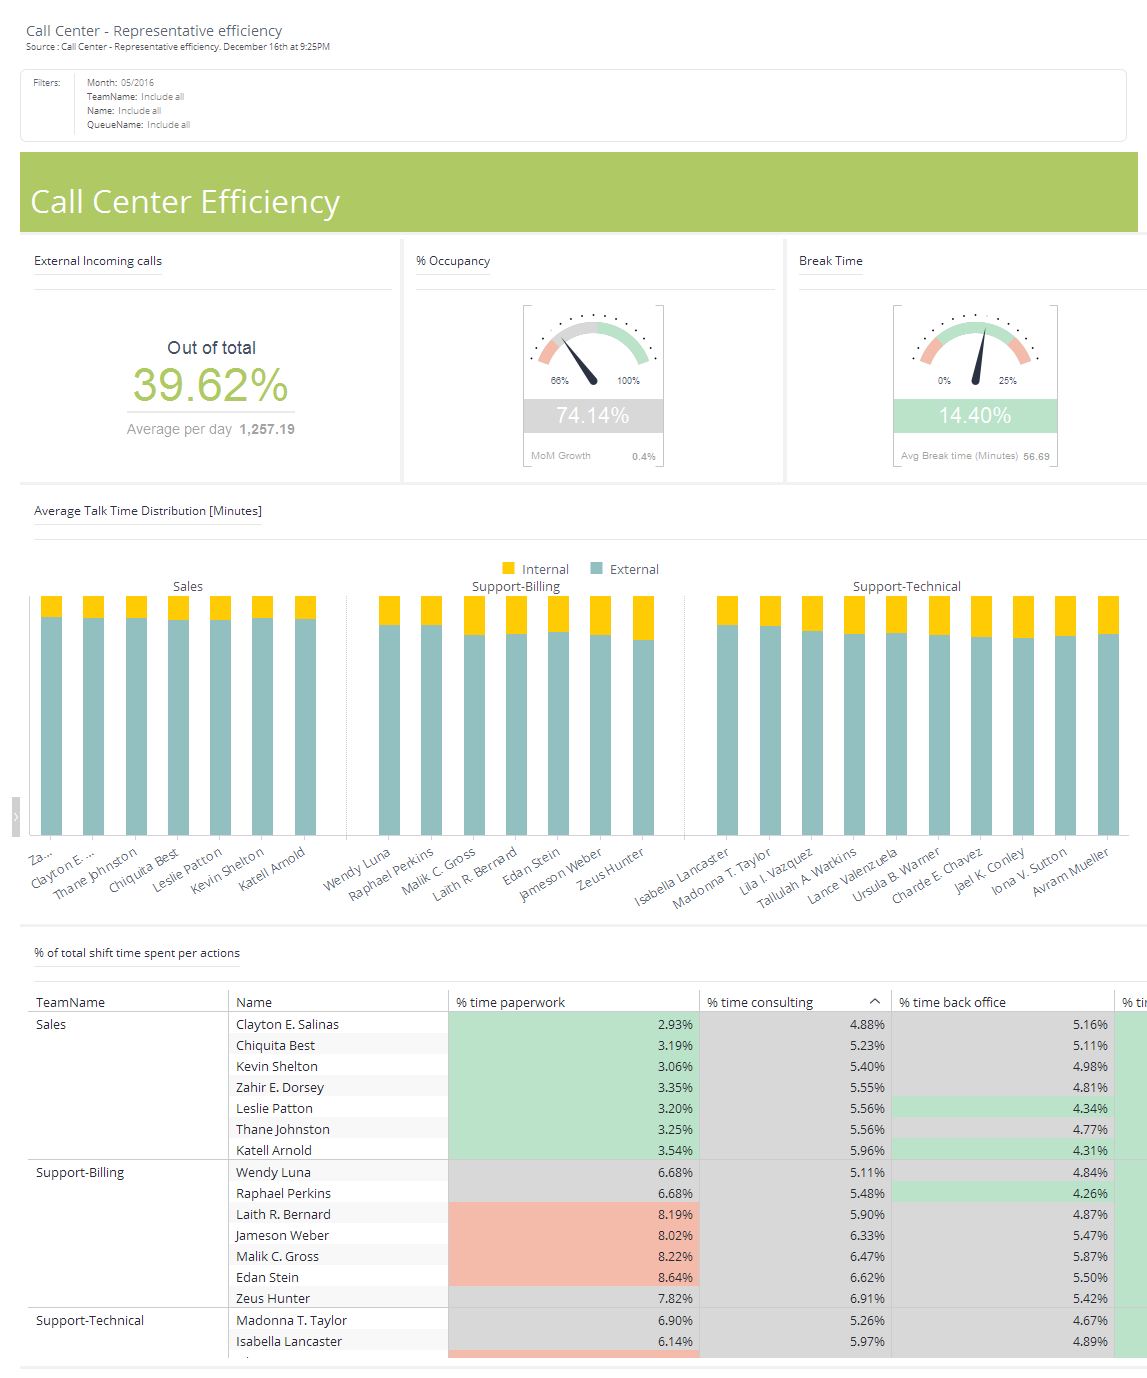
\includegraphics{call.png}
\caption{}
\end{figure}

\subsection{Increase profit margins}\label{increase-profit-margins}

Goals:

\begin{itemize}
\tightlist
\item
  Allow the CFO of the company to compare the net profit margin over
  time and relative to other companies in the same sector.
\item
  Allow investors to compare the net profit margin across industries to
  identify the most profitable and attractive sectors and companies to
  invest in
\end{itemize}

\begin{figure}
\centering
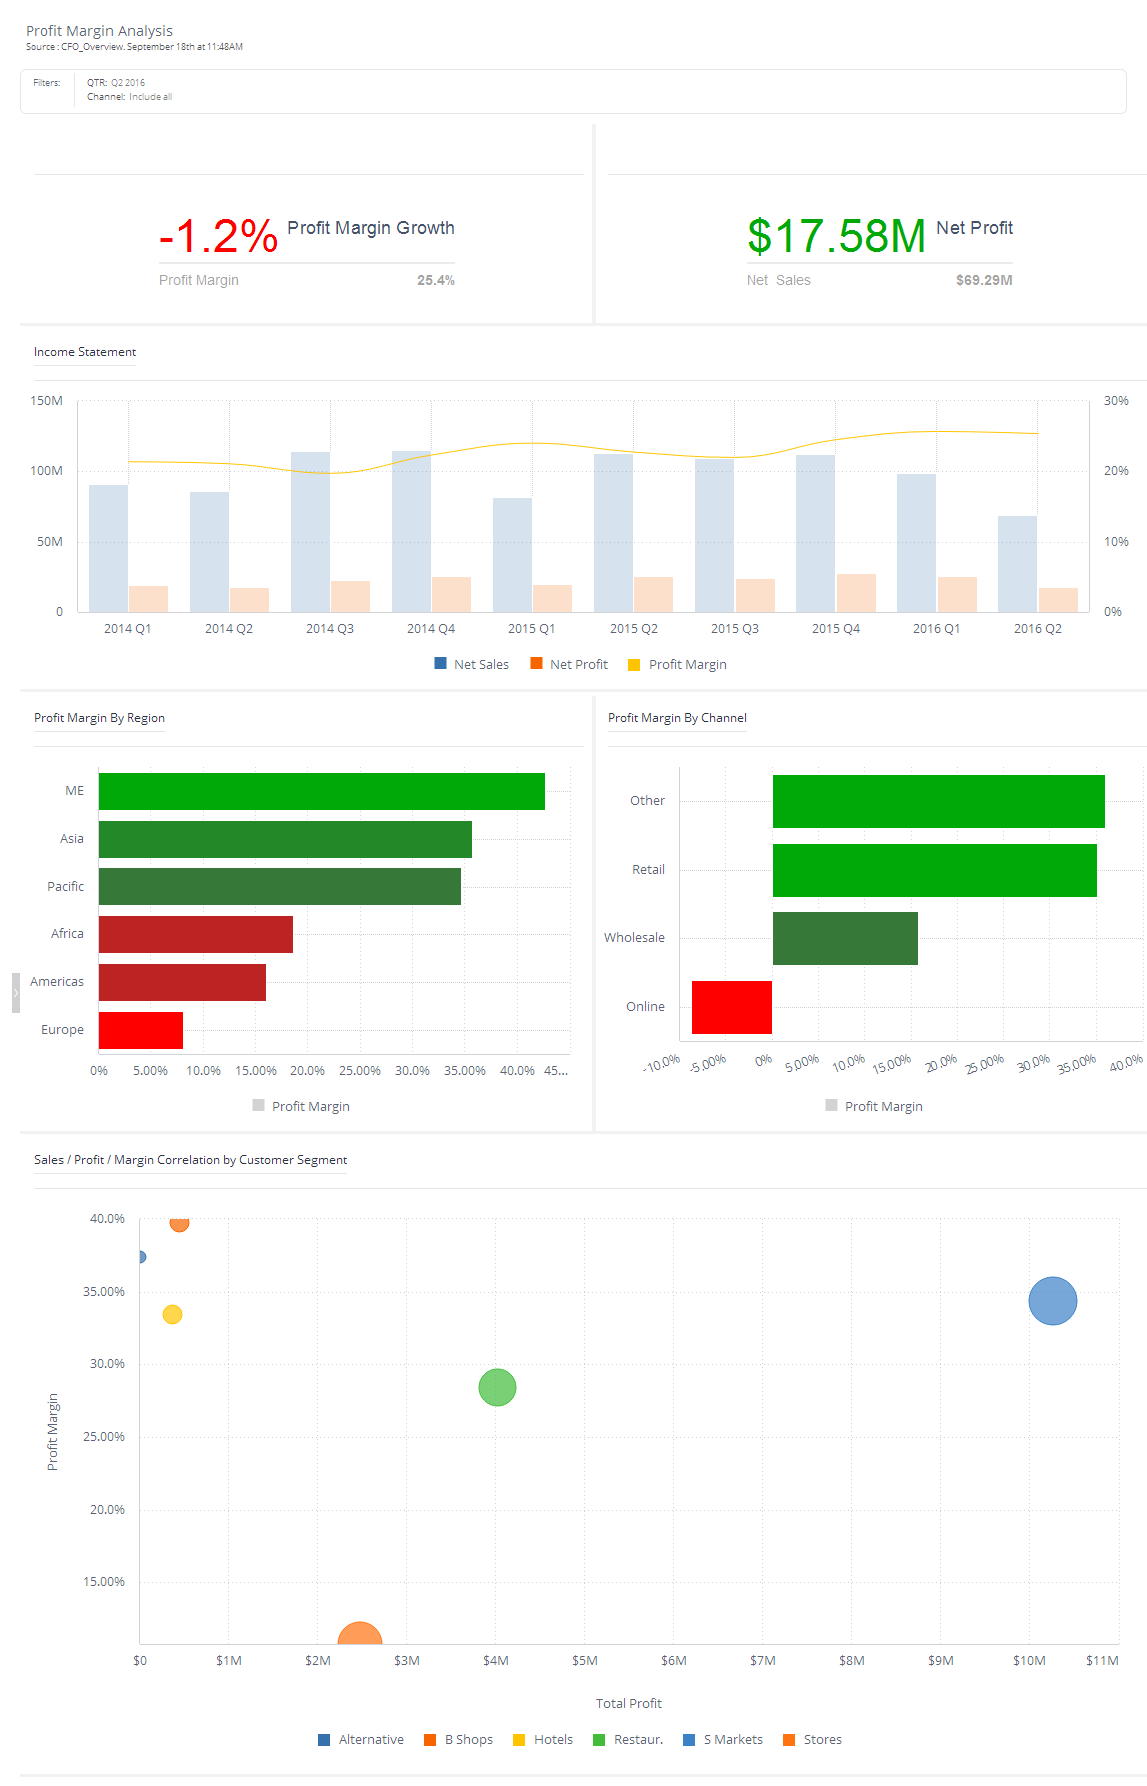
\includegraphics{increaseprofit.png}
\caption{}
\end{figure}

\subsection{Optimize campaigns}\label{optimize-campaigns}

Goals: Increase sales originating from our online marketing activity.

\begin{figure}
\centering
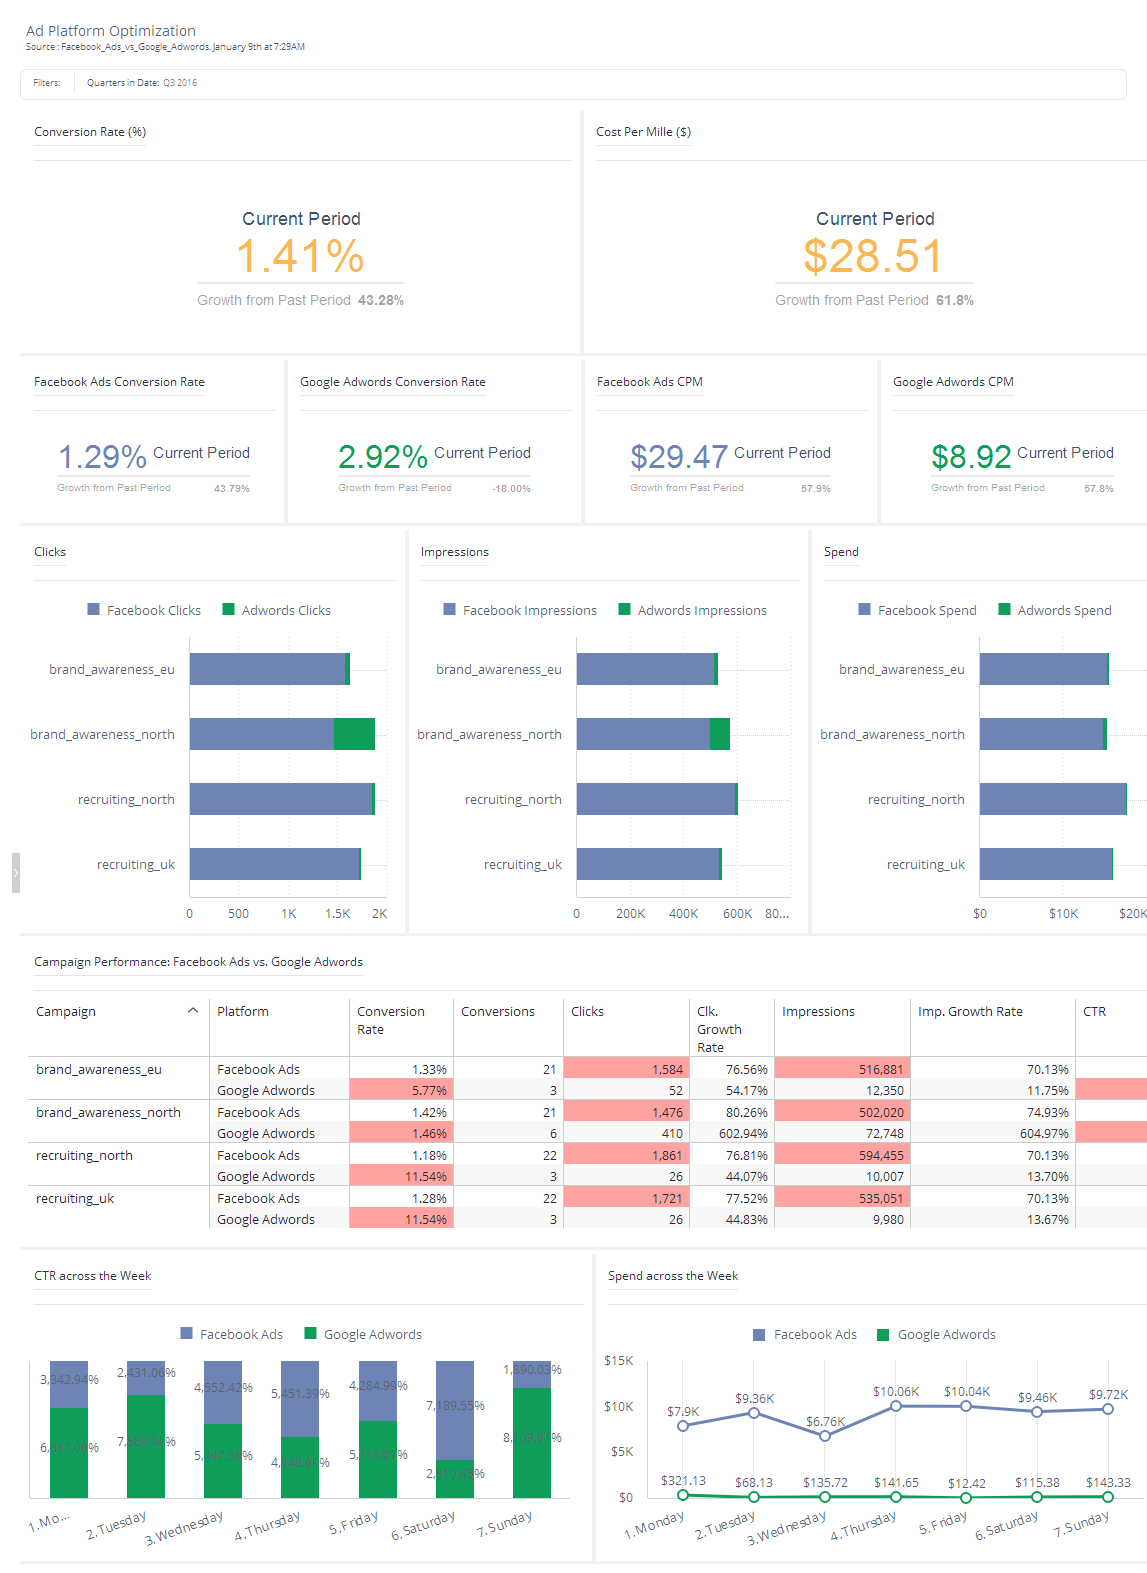
\includegraphics{campaigns.png}
\caption{}
\end{figure}

\section{By Department}\label{by-department}

\subsection{Sales}\label{sales}

Example KPIs for Sales Departments:

\begin{itemize}
\tightlist
\item
  Actual calls
\item
  Actual sales value versus initial bid
\item
  Age of sales forecast
\item
  Average administrative time per sales person
\item
  Average deal size
\item
  Average number of activities (calls, meetings, etc.) to close a deal
\item
  Average price discount per product
\item
  Average price discount per sales person
\item
  Average revenue per product
\item
  Call quota
\item
  Closed sales
\item
  Closing ratio
\item
  Customer acquisitions costs as a percentage of sales value
\item
  Customer churn ratio
\item
  Customer loyalty
\item
  Customer purchase frequency
\item
  Customer satisfaction
\item
  Frequency of sales transactions
\item
  Gross margin per product
\item
  Gross margin per sales person
\item
  New sales person ramp-up time
\item
  Number of certified partners
\item
  Number of deals per partner
\item
  Number of sales orders by FTE
\item
  Number of sales people meeting their quota
\item
  Number of units sold per day/week/month/quarter/year
\item
  Partner churn ratio
\item
  Partner profit margin
\item
  Percentage of converted opportunities
\item
  Percentage of online sales revenue
\item
  Percentage of sales due to launched product/services
\item
  Percentage of sales representatives to achieve quota
\item
  Percentage of sales revenue via partner channel
\item
  Pipeline by sales stage
\item
  Qualified leads
\item
  Qualified opportunities
\item
  Revenue per sales person
\item
  Sales capacity
\item
  Sales cycle time
\item
  Sales per department
\item
  Sales person turnover
\item
  Sales quota
\item
  Time utilization
\item
  Unweighted sum of deal size in sales pipeline
\item
  Value of sales lost
\item
  Win/loss ratio percentage
\end{itemize}

\subsection{Marketing}\label{marketing}

Example KPIs for Marketing Departments:

\begin{itemize}
\tightlist
\item
  Ad click-through ratio (CTR)
\item
  Average response rates of campaigns
\item
  Brand awareness percentage
\item
  Brand consideration
\item
  Brand credibility
\item
  Brand strength
\item
  Column inches of media coverage
\item
  Consumer awareness
\item
  Contact rate (number of contacts effectively contacted / number of
  contacts in the target list)
\item
  Cost per converted lead
\item
  Cost per lead
\item
  Cost per mille (CPM)
\item
  Delivery of materials
\item
  Effective reach
\item
  Gross rating point (GRP)
\item
  Growth sustainability rate of brand
\item
  Leads generated
\item
  Marketing budget awareness-demand ratio
\item
  Marketing budget ratio (MER)
\item
  Number of article placements in trade magazines
\item
  Number of client visits
\item
  Number of product focus groups conducted
\item
  Number of customer satisfaction surveys administered
\item
  Number of placements in trade magazines
\item
  Number of trade shows attended / participated in
\item
  Percentage of customers willing to promote your product/service
\item
  Q score (a way to measure the familiarity and appeal of a brand, etc.)
\item
  Response rate
\item
  Return on investment (ROI) of brand
\item
  Return on marketing investment (ROMI)
\item
  Revenue generation capabilities of brand
\item
  Staying in budget
\item
  Target rating point
\item
  Total cost of customer acquisition
\item
  Transaction value of brand
\item
  Website click-throughs
\item
  Website hits
\item
  Website leads generated
\end{itemize}

\subsection{Finance}\label{finance}

Example KPIs for Finance Departments:

\begin{itemize}
\tightlist
\item
  Accounting costs
\item
  Accounts payable turnover
\item
  Accounts receivable collection period
\item
  Accounts receivable turnover
\item
  Actual expenses
\item
  Amount due (per customer)
\item
  Average customer receivable
\item
  Average monetary value of invoices outstanding
\item
  Average monetary value of overdue invoices
\item
  Average number of trackbacks per post
\item
  Budget variance for each key metric
\item
  Budgeted expenses
\item
  Capital expenditures
\item
  Cash conversion cycle (CCC)
\item
  Cash flow return on investments (CFROI)
\item
  Cost of goods sold (COGS)
\item
  Cash dividends paid
\item
  Cost per pay slip issued
\item
  Creditor days
\item
  Current receivables
\item
  Cumulative annual growth rate (CAGR)
\item
  Cycle time for expense reimbursements
\item
  Cycle time to process payroll
\item
  Cycle time to resolve an invoice error
\item
  Cycle time to resolve payroll errors
\item
  Days payable
\item
  Debtor days
\item
  Direct cost
\item
  Discounted cash flow
\item
  Earnings before interest and taxes (EBIT)
\item
  Earnings before interest, taxes, depreciation (EBITDA)
\item
  Economic value added (EVA)
\item
  Employee available time
\item
  Employee scheduled time
\item
  Employee work center loading
\item
  Enterprise value/ takeover value
\item
  Expense account credit transactions
\item
  Expense account debit transactions
\item
  Expense account transactions
\item
  Fixed costs
\item
  Gross profit
\item
  Gross profit margin
\item
  Indirect costs
\item
  Inventory turnover
\item
  Inventory value
\item
  Invoice processing costs
\item
  Internal rate of return (IRR)
\item
  Market share gain comparison percentage
\item
  Net change in cash
\item
  Net income
\item
  Net present value (NPV)
\item
  Number of invoices outstanding
\item
  Number of unapplied receipts
\item
  Number of past-due loans
\item
  Open receivables
\item
  Open receivables amount (per customer)
\item
  Operating leverage
\item
  Past-due receivables
\item
  Payables turnover
\item
  Payment errors as a percentage of total payroll disbursement
\item
  Percentage accuracy of financial reports
\item
  Percentage of bad debts against invoiced revenue
\item
  Percentage of electronic invoices
\item
  Percentage in dispute (per customer)
\item
  Percentage of invoices being queried
\item
  Percentage of invoices requiring special payment
\item
  Percentage of low-value invoices
\item
  Percentage of open receivables (per customer)
\item
  Percentage of payable invoices without purchase order
\item
  Percentage of service requests posted via web (self-help)
\item
  Perfect order measure
\item
  Quick ratio
\item
  Receivables
\item
  Receivables turnover
\item
  Return on capital employed (ROCE)
\item
  Sales growth
\item
  Share price
\item
  Systems cost of payroll process as a percentage of total payroll cost
\item
  Total payables
\item
  Total energy used per unit of production
\item
  Total receivables
\item
  Total sales
\item
  Unapplied receipts
\item
  Variable costs
\item
  Weighted days delinquent sales outstanding
\item
  Weighted days delinquent sales outstanding (per customer)
\item
  Weighted terms outstanding
\item
  Weighted terms outstanding (per customer)
\end{itemize}

\subsection{Human Resources}\label{human-resources}

Example KPIs for Human Resources (HR) Departments:

\begin{itemize}
\tightlist
\item
  Actual versus budgeted cost of hire
\item
  Annualized voluntary employee turnover rate
\item
  Annualized voluntary turnover rate
\item
  Average headcount of employees each human resources (HR) employee
  working is caring for
\item
  Average interviewing costs
\item
  Average length of placement in months for the manager
\item
  Average length of service of all current employees
\item
  Average length of service of all employees who have separated
\item
  Average months placement
\item
  Average number of training hours per employee
\item
  Average number of vacation days per employee
\item
  Average performance scores of departing employees
\item
  Average retirement age
\item
  Average salary
\item
  Average salary for all employees reporting to the selected manager
\item
  Average sourcing cost per hire
\item
  Average time employees are in same job/ function
\item
  Average time to competence
\item
  Average time to update employee records
\item
  Average training costs per employee
\item
  Compensation cost as a percentage of revenue
\item
  Contingent workers
\item
  Employee satisfaction with training
\item
  End placements
\item
  Female to male ratio
\item
  Full-time employees (FTEs) per human resources (HR) department FTE
\item
  Headcount of contingent workers for the manager
\item
  HR average years of service (incumbents)
\item
  HR average years of service (terminations)
\item
  HR department cost per FTE
\item
  HR headcount - Actual
\item
  HR headcount - Available
\item
  HR to employee staff ratio
\item
  Job vacancies as a percentage of all positions
\item
  New hire quality
\item
  Time to fill
\item
  Hiring manager satisfaction
\item
  Cost per hire
\item
  Staffing efficiency
\item
  Internal, external, and total headcount recruiting costs and ratios
\item
  Number of end placements made in the reporting period for the manager
\item
  Part-time employees as a percentage of total employees
\item
  Percentage of employees receiving regular performance reviews
\item
  Percentage of employees that are near or at max for their vacation
  balances
\item
  Percentage of HR budget spent on training
\item
  Percentage of new hire retention
\item
  Ratio of internal versus external training
\item
  Ratio of standard level wage to local minimum wage
\item
  Return on investment (ROI) of training
\item
  Total overtime hours as a percentage of all work hours
\item
  Training penetration rate (percentage of employees completing a course
  compared to all FTEs)
\item
  Workforce stability
\end{itemize}

\subsection{Information Technology}\label{information-technology}

Example KPIs for Information Technology (IT) Departments:

\begin{itemize}
\tightlist
\item
  Account create success
\item
  Account termination success
\item
  Active directory performance index
\item
  Alert-to-ticket ratio
\item
  Average data center availability
\item
  Call center PBX availability
\item
  Campus PBX availability
\item
  Customer connection effectiveness
\item
  Data center capacity consumed
\item
  Email client availability
\item
  Exchange server availability
\item
  Incidents from change
\item
  Internet proxy performance
\item
  Network availability - High availability sites
\item
  Network availability - Standard sites
\item
  Network manageability index
\item
  No problem found/duplicate tickets
\item
  Percentage of branch office backup success
\item
  Percentage of circuits exceeding target utilization
\item
  Percentage of IT managed servers patched at deadline
\item
  Percentage of production servers meeting software configuration
  standards
\item
  Percentage of security update restarts within maintenance window
\item
  Percentage successful remote access server (RAS) connections
\item
  Phone answer service level
\item
  Priority 1 and priority 2 network incidents meeting SLA
\item
  Product adoption status and compliance
\item
  Restore success rate
\item
  Server growth rate
\item
  Server manageability index
\item
  Service desk client satisfaction - Percentage dissatisfied
\item
  Service desk tier 1 resolution rate
\item
  Service desk time to escalate
\item
  Service desk time to resolve
\item
  Storage utility service availability
\item
  Storage utility utilization
\item
  Virtual machine provisioning interval
\item
  Virtual server utility availability
\item
  Web server availability
\end{itemize}

\subsection{Customer Service}\label{customer-service}

Example KPIs for Customer Service Departments

\begin{itemize}
\tightlist
\item
  Agent's full-time employees (FTEs) as percentage of total call center
  FTEs
\item
  Answering percentage (number of sales calls answered/total number of
  sales calls offered)
\item
  Average after-call work time
\item
  Average number of calls/ service request per handler
\item
  Average queue time of incoming phone calls
\item
  Cost per minute of handle time
\item
  Costs of operating call center/ service desk
\item
  Email backlog
\item
  Field service technician utilization
\item
  Hit rate (products sold compared to total received sales calls)
\item
  Inbound abandon rate
\item
  Inbound agent dialed calls
\item
  Inbound availability rate
\item
  Inbound average talk time
\item
  Inbound average wrap time
\item
  Inbound call center leads created
\item
  Inbound call center opportunities created
\item
  Inbound calls handled
\item
  Inbound calls handled per agent hour
\item
  Inbound service level
\item
  Number of complaints
\item
  Percentage of customer service requests answered in given timeframe
\item
  Percentage of calls transferred
\item
  Total calling time per day/week/month
\end{itemize}

\chapter{Deutsche Bahn Use Case}\label{deutsche-bahn-use-case}

DB Headquarters has the consulting function for all of DB Subdiaries. DB
Headquarters works together with the all data sources to devise data
usage strategies. By collaborating with the domain's experts, DB
Headquarters develops matching mathematical models and realises the
application environment. The data and corresponding analytical results
are then prepared for visual presentation and made available for further
examination.

At Deutsche Bahn the using of KPI have three functions:

\begin{enumerate}
\def\labelenumi{\arabic{enumi}.}
\tightlist
\item
  General Overview
\item
  Warning system
\item
  Decisions making
\end{enumerate}

Below are some of use case in DB:

\section{IT Spend Analysis KPI}\label{it-spend-analysis-kpi}

\textbf{Overview:}

The IT Spend Analysis Dashboard analyze the planned vs.~actual costs of
an IT department. This Dashboard comparison helps us understand how well
the company planned for the year and investigate areas with huge
deviations from the plan.

\textbf{Glossary:}

\begin{quote}
Year-to-date (YTD) is a period, starting from the beginning of the
current year (either the calendar year or fiscal year) and continuing up
to the present day.
\end{quote}

\begin{quote}
Var: Variance or the deviation
\end{quote}

\textbf{Dataset:}

This data is part of a series that illustrates how you can Dashboard BI
with business-oriented data, reports and dashboards. This is real data
from obviEnce (\url{http://obvience.com/}) that has been anonymized.

This analysis contains 8 entity (table) and every table has attribute.

\begin{enumerate}
\def\labelenumi{\arabic{enumi}.}
\tightlist
\item
  business area
\end{enumerate}

\begin{itemize}
\tightlist
\item
  Attribute: Business Area, Business Area ID,
\end{itemize}

\begin{enumerate}
\def\labelenumi{\arabic{enumi}.}
\setcounter{enumi}{1}
\tightlist
\item
  cost element
\end{enumerate}

\begin{itemize}
\tightlist
\item
  Attribute: Cost element name, Cost Element Group, Cost Element Sub
  Group, Cost Element ID
\end{itemize}

\begin{enumerate}
\def\labelenumi{\arabic{enumi}.}
\setcounter{enumi}{2}
\tightlist
\item
  country region
\end{enumerate}

\begin{itemize}
\tightlist
\item
  Attribute: Sales Region, Country/Region, Country/Region ID
\end{itemize}

\begin{enumerate}
\def\labelenumi{\arabic{enumi}.}
\setcounter{enumi}{3}
\tightlist
\item
  date
\end{enumerate}

\begin{itemize}
\tightlist
\item
  Attribute: Date, Year, Period, Month
\end{itemize}

\begin{enumerate}
\def\labelenumi{\arabic{enumi}.}
\setcounter{enumi}{4}
\tightlist
\item
  department
\end{enumerate}

\begin{itemize}
\tightlist
\item
  Attribute: VP, Department
\end{itemize}

\begin{enumerate}
\def\labelenumi{\arabic{enumi}.}
\setcounter{enumi}{5}
\tightlist
\item
  it-area
\end{enumerate}

\begin{itemize}
\tightlist
\item
  Attribute: IT Area, IT Sub Area, IT Sub Area ID
\end{itemize}

\begin{enumerate}
\def\labelenumi{\arabic{enumi}.}
\setcounter{enumi}{6}
\tightlist
\item
  scenario
\end{enumerate}

\begin{itemize}
\tightlist
\item
  Attribute: Scenario, Scenario ID, ScenarioDescription
\end{itemize}

\begin{enumerate}
\def\labelenumi{\arabic{enumi}.}
\setcounter{enumi}{7}
\tightlist
\item
  fact\_it
\end{enumerate}

\begin{itemize}
\tightlist
\item
  Attribute: Date, Value, Department, Cost Element ID, Country/Region
  ID, Business Area ID, IT Sub Area ID, Scenario ID
\end{itemize}

\textbf{Solution:}

IT Spend Trend Dashboard: YTD IT Spend Trend Analysis page

\begin{itemize}
\tightlist
\item
  Var Plan \% by Sales Region
\item
  Var Plan by Month
\item
  Var Plan , Var Plan \% and Actual by Business Area and Period
\item
  IT Area
\end{itemize}

Spend by Cost Element Dashboard: YTD Spend by Cost Elements page

\begin{itemize}
\tightlist
\item
  Plan and Target
\item
  Var Plan \% and Var LE3 \% by IT Area
\item
  Var Plan \% by Sales Region
\item
  Amount by Month and Scenario
\end{itemize}

Plan Variance Analysis Dashboard

\begin{itemize}
\tightlist
\item
  Variance Latest Estimates
\item
  Var Plan \% by Business Area
\item
  Var Plan by Sales Region
\item
  Var Plan \% by Month and Business Area
\end{itemize}

\textbf{Technical documentation: }

Let's make the data model from the 8 entity. Just drag every
\href{https://en.wikipedia.org/wiki/Primary_key}{Primary Key} of the
entity in power pivot or power bi data model

\begin{figure}
\centering
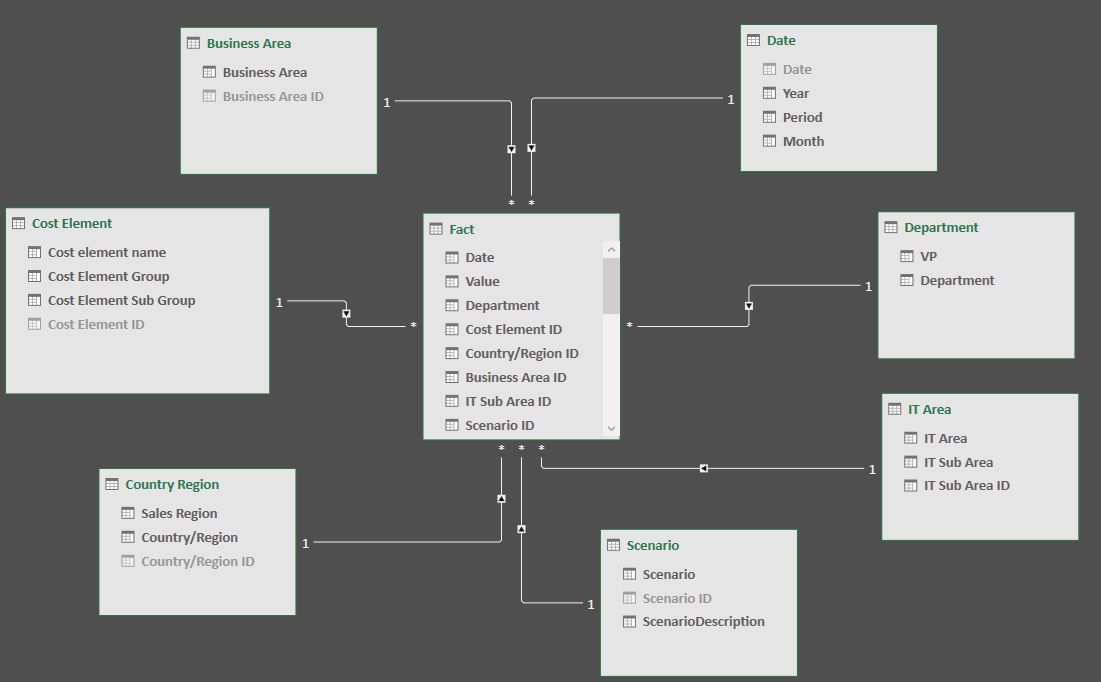
\includegraphics{itspend.PNG}
\caption{}
\end{figure}

After that, create
\href{https://docs.microsoft.com/en-us/power-bi/desktop-tutorial-create-measures}{a
measure in power bi or power pivot}

\textbf{Note:} we use the format of table and attribut with
\href{https://docs.microsoft.com/en-us/power-bi/desktop-quickstart-learn-dax-basics}{DAX
language}

\textbf{Extras:}
\href{https://support.office.com/en-us/article/quickstart-learn-dax-basics-in-30-minutes-51744643-c2a5-436a-bdf6-c895762bec1a?omkt=en-US\&ui=en-US\&rs=en-US\&ad=US}{Quick
Guide DAX}

Below are the explanation of every graph:

\section{Human Resources KPI}\label{human-resources-kpi}

\textbf{Overview: }

Human Resources (HR) dashboards aggregate and present employee data in a
meaningful way. As a metrics, Human Resources dashboards simplify
information gathering, and present data in a way that can be sorted,
analyzed, and presented. This use case dashboard looks at new hires,
active employees, and employees who left and tries to uncover any trends
in the hiring strategy. Our main objectives are to understand:

\begin{itemize}
\tightlist
\item
  Who we hire
\item
  Biases in our hiring strategy
\item
  Trends in voluntary separations
\end{itemize}

\textbf{Glosarry: }

\begin{quote}
SPLY: same periode last year. One year back in time from the context
dates
\end{quote}

\textbf{Dataset: }

This Human Resources data is part of a series that illustrates how you
can Dashboard BI with business-oriented data, reports and dashboards.
This is real data from obviEnce (\url{http://obvience.com/}) that has
been anonymized.

This dataset contains 9 entity (table) and every table has attribute to.

\begin{enumerate}
\def\labelenumi{\arabic{enumi}.}
\tightlist
\item
  age group
\end{enumerate}

\begin{itemize}
\tightlist
\item
  Attribute: AgeGroupID, AgeGroup
\end{itemize}

\begin{enumerate}
\def\labelenumi{\arabic{enumi}.}
\setcounter{enumi}{1}
\tightlist
\item
  gender
\end{enumerate}

\begin{itemize}
\tightlist
\item
  Attribute: ID, Gender, Sort
\end{itemize}

\begin{enumerate}
\def\labelenumi{\arabic{enumi}.}
\setcounter{enumi}{2}
\tightlist
\item
  ethnicity Attribute: Ethnic Group, Ethnicity
\item
  date Attribute: Date, Month, MonthNumber, Period, PeriodNumber, Qtr,
  QtrNumber, Year, Day, MonthStartDate, MonthEndDate,
  MonthIncrementNumber
\item
  separation reason Attribute: SeparationTypeID, SeparationReason
\item
  pay type Attribute: PayTypeID, PayType
\item
  FP
\end{enumerate}

\begin{itemize}
\tightlist
\item
  Attribute: FP, FPDesc
\end{itemize}

\begin{enumerate}
\def\labelenumi{\arabic{enumi}.}
\setcounter{enumi}{7}
\tightlist
\item
  bu Attribute: BU, RegionSeq, VP, Region
\end{enumerate}

\begin{itemize}
\tightlist
\item
  employee\_fact Attribute: date, EmplID, Gender, Age, EthnicGroup, FP,
  TermDate, isNewHire, BU, HireDate, PayTypeID, TermReason, AgeGroupID
  ,TenureDays, TenureMonths, BadHires
\end{itemize}

\textbf{Solution: }

New hires Dashboard

\begin{itemize}
\tightlist
\item
  New Hires Vs New Hires SPLY
\item
  New Hires by Region and FPDesc
\item
  New Hires by Region and Ethnicity
\item
  Gender
\item
  AgeGroup
\end{itemize}

Active Employees vs Separations Dashboard

\begin{itemize}
\tightlist
\item
  YoY Change
\item
  AgeG roup
\item
  Gender
\item
  Actives by Region
\item
  Actives vs Actives SPLY
\item
  Separations by Reason
\item
  Seps vs Seps SPLY
\end{itemize}

Bad Hires Dashboard

Bad hires are defined as employees who didn't last for more than 60
days.

\begin{itemize}
\tightlist
\item
  Bad Hires by Region and Gender
\item
  Bad Hires by Region and Ethnicity
\item
  Bad Hires YoY \% Change by Month and Age Group
\item
  Bad Hire \% of Actives and Bad Hires \% of Active SPLY by Region
\end{itemize}

\textbf{Technical Documentation: }

\section{Opportunity Analysis KPI}\label{opportunity-analysis-kpi}

\textbf{Overview :}

Opportunity analyisis is a detailed review of the prospects within a
potential market. The company has 2 sales channels: direct and partner.
The Sales Department created this dashboard to track opportunities and
revenue by region, deal size, and channel.

The Sales Department relies on two measures of revenue:

\begin{itemize}
\tightlist
\item
  \textbf{Revenue }-- this is a salesperson's estimate of what he
  believes the revenue will be.
\item
  \textbf{Factored Revenue } -- this is calculated as Revenue X
  Probability\% and is generally accepted as being a more-accurate
  predictor of actual sales revenue. Probability is determined by the
  deal's current \textbf{Sales Stage }.

  \begin{itemize}
  \tightlist
  \item
    Lead -- 10\%
  \item
    Qualify -- 20\%
  \item
    Solution -- 40\%
  \item
    Proposal -- 60\%
  \item
    Finalize -- 80\%
  \end{itemize}
\end{itemize}

\textbf{Glossary: }

\begin{quote}
AVG: Average
\end{quote}

\textbf{Dataset : }

This data is part of a series that illustrates how you can Dashboard BI
with business-oriented data, reports and dashboards. This is real data
from obviEnce (\url{http://obvience.com/}) that has been anonymized.

This dataset contains 5 entity (table) and every table has attribute.

\begin{enumerate}
\def\labelenumi{\arabic{enumi}.}
\tightlist
\item
  sales stage
\end{enumerate}

\begin{itemize}
\tightlist
\item
  Attibute: Probability, Sales Stage, Sales Stage ID
\end{itemize}

\begin{enumerate}
\def\labelenumi{\arabic{enumi}.}
\setcounter{enumi}{1}
\tightlist
\item
  product
\end{enumerate}

\begin{itemize}
\tightlist
\item
  Attibute: Product Code, Product ID
\end{itemize}

\begin{enumerate}
\def\labelenumi{\arabic{enumi}.}
\setcounter{enumi}{2}
\tightlist
\item
  partner
\end{enumerate}

\begin{itemize}
\tightlist
\item
  Attibute: Partner, Partner ID, Partner Driven
\end{itemize}

\begin{enumerate}
\def\labelenumi{\arabic{enumi}.}
\setcounter{enumi}{3}
\tightlist
\item
  opportunity
\end{enumerate}

\begin{itemize}
\tightlist
\item
  Attibute: Name, Opportunity ID, Rank, SizeID, Opportunity Size
\end{itemize}

\begin{enumerate}
\def\labelenumi{\arabic{enumi}.}
\setcounter{enumi}{4}
\tightlist
\item
  fact
\end{enumerate}

\begin{itemize}
\tightlist
\item
  Attibute: EstimatedCloseDate, Opportunity ID, Sales Stage ID, Account
  ID, Partner ID, Product ID, ProductRevenue, FactoredProductRevenue,
  Create Date, Opportunity Days, Year, Month\_Number, Month
\end{itemize}

\textbf{Solution : }

Opportunity Counts Overview

\begin{itemize}
\tightlist
\item
  Opportunity Count
\item
  Opportunity Count by Region
\item
  Opportunity Count by Sales Stage
\item
  Opportunity Count by Partner Driven and Opportunity Size
\item
  Opportunity Count by Partner Driven and Sales Stage
\end{itemize}

Revenue Analysis

\begin{itemize}
\tightlist
\item
  Revenue by Region
\item
  Revenue by Sales Stage and Partner Driven
\item
  Revenue
\item
  Factored Revenue
\item
  Opportunity Count
\item
  AVG Revenue by Partner Driven and Opportunity Size
\end{itemize}

Upcoming Opportunities by Month

\begin{itemize}
\tightlist
\item
  Opportunity Count
\item
  Factored Revenue by Opportunity Size
\item
  AVG Revenue by Partner Driven and Sales Stage
\item
  Opportunity Count by Month and Sales Stage
\end{itemize}

\textbf{Technical Documentation: }

\section{Data Science HR Turnover}\label{data-science-hr-turnover}

\section{Data Science Sales
Prediction}\label{data-science-sales-prediction}

{[}1{]} Schmidt, Klaus D, 2005, Versicherungsmathematik, Springer
Lehrbuch, Springer Verlag

{[}2{]} Beate, Bergter, WS 2013, Formelsammlung
Wahscheinlichkeitsrechnung, HTW Berlin, Deutschland

\chapter{Appendix}\label{appendix}

\bibliography{book.bib,packages.bib}


\end{document}
